\chapter{MC samples and selection}
    \chapterprecishere{
        ``Potentielle citation sans aucun rapport avec le sujet"\par\raggedleft--- \textup{Personne inconnue}, contexte à déterminer
    }
    
    
    \section{Data and MC samples}
    The data and MC samples for this study were collected under special beam conditions that ensure low pile-up. The data samples were collected in three runs:
    \begin{itemize}
    \item $\sqrt{s} = 5.02\tev$ data taken in November 2017, ATLAS data
    period M, preliminary calibrated luminosity $256.827\,\ipb$ with an uncertainty
    of $\pm 1.6\%$
    \item $\sqrt{s} = 13\tev$ data taken in November 2017, ATLAS data
    period N, preliminary online luminosity $146.6\ipb$
    \item $\sqrt{s} = 13\tev$ data taken in June 2018, ATLAS data
    period G4+J, preliminary online luminosity $193.2\ipb$
    \end{itemize}
	The runs of November 2017 and the run of June 2018 had the same bunch spacing of 25 ns, but a different filling scheme. The two main differences from the high-$\mu$ data collection are the following:
	\begin{itemize}
	\item In order to optimize topo-cluster response for the \gls{hr} lower topo-cluster thresholds were used. 
	\item Single $e$ and $\mu$ triggers with significantly lower
	thresholds and looser identification criteria are run without
	prescale, most notably \texttt{HLT\_e15\_lhloose\_nod0\_L1EM12} and
	\texttt{HLT\_mu14}.
	\end{itemize}	
	At the beginning of 5 TeV fills the pile-up reached $\mu \backslash 5$, slowly descending to $\mu \backslash 1$ by the end of the run. In the case of 13 TeV the luminosity was levelled at $\mu = 2$ in the course of the run. The corresponding distributions for $\mu$ and $N_{PV}$ for the 5 TeV and 13 TeV runs are shown in Fig. \ref{fig:mu5} and Fig. \ref{fig:mu13}.
	\begin{figure}[tph]
		\centering
		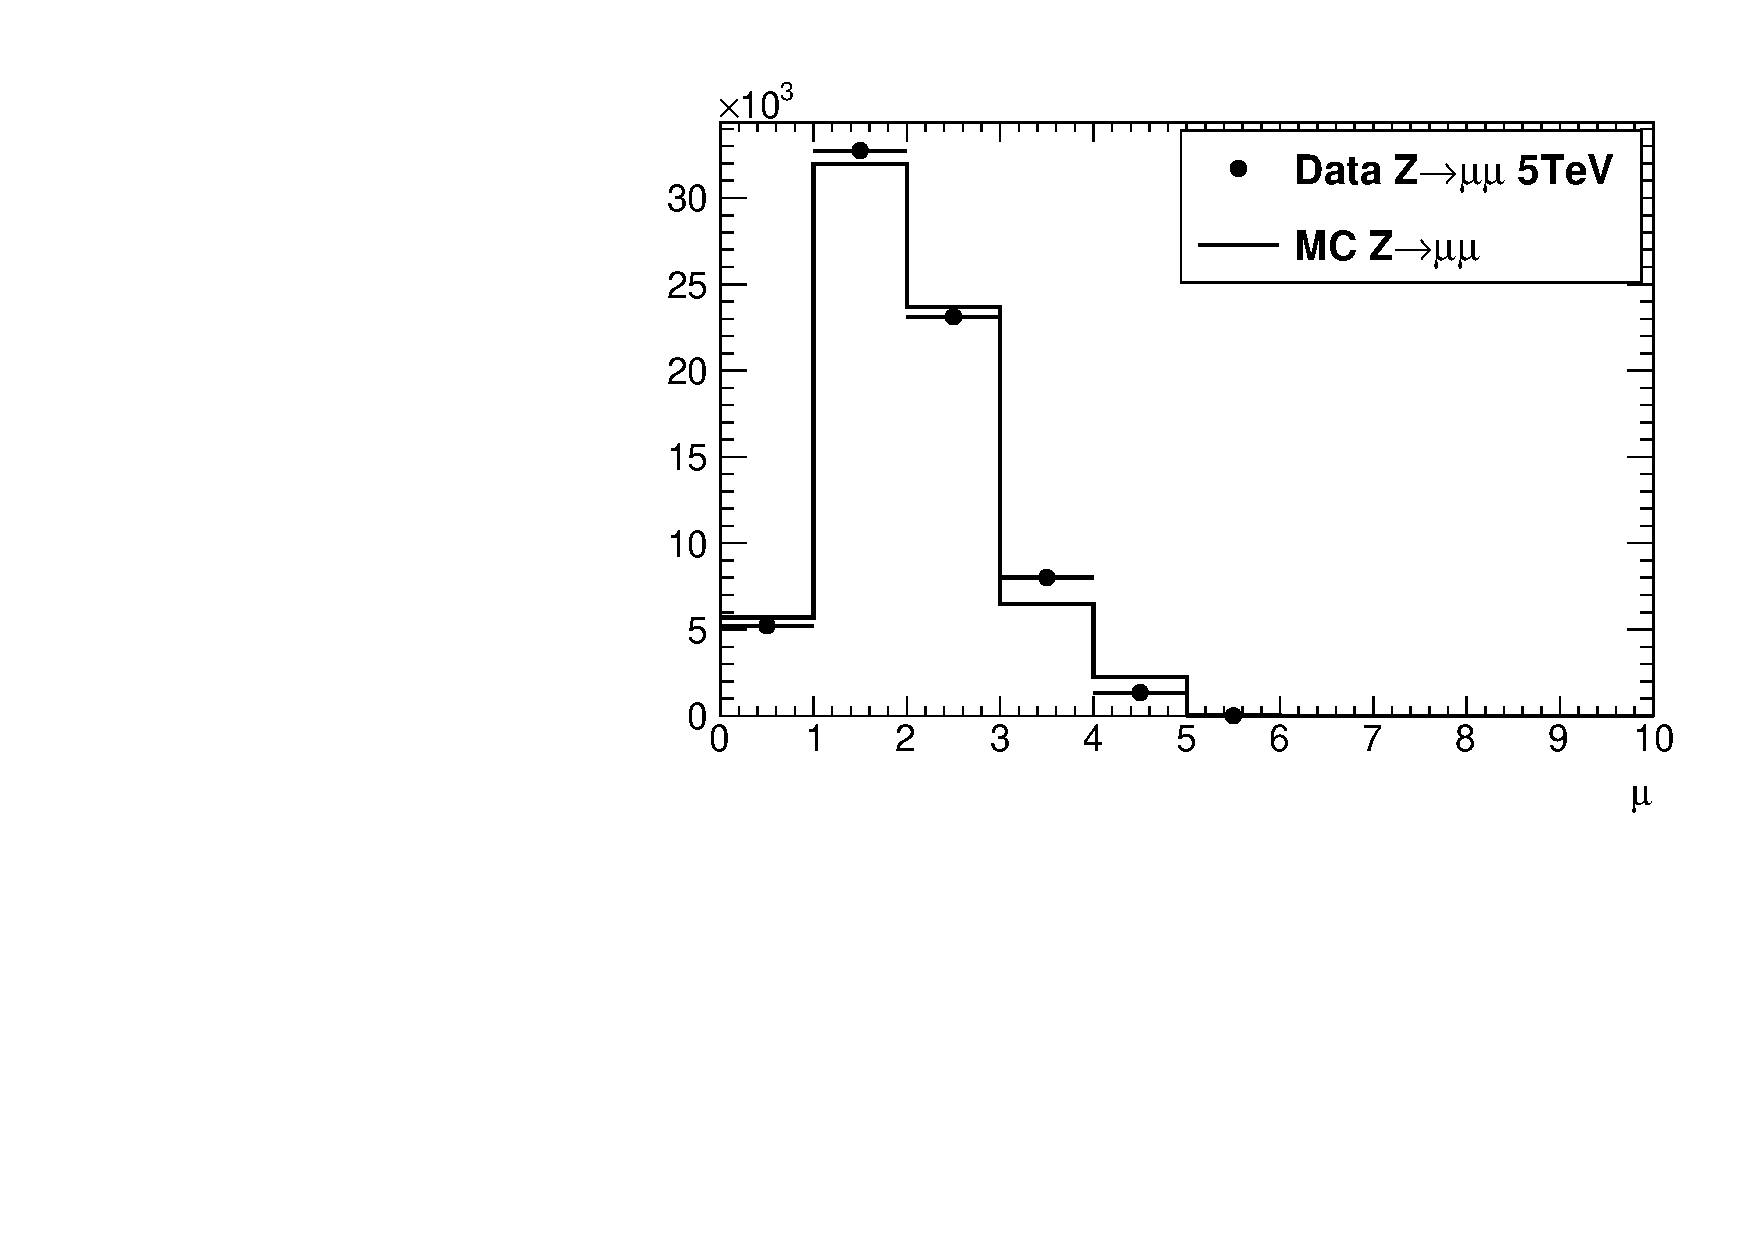
\includegraphics[width=.33\textwidth]{zmumu_5tev_mu.pdf}%
		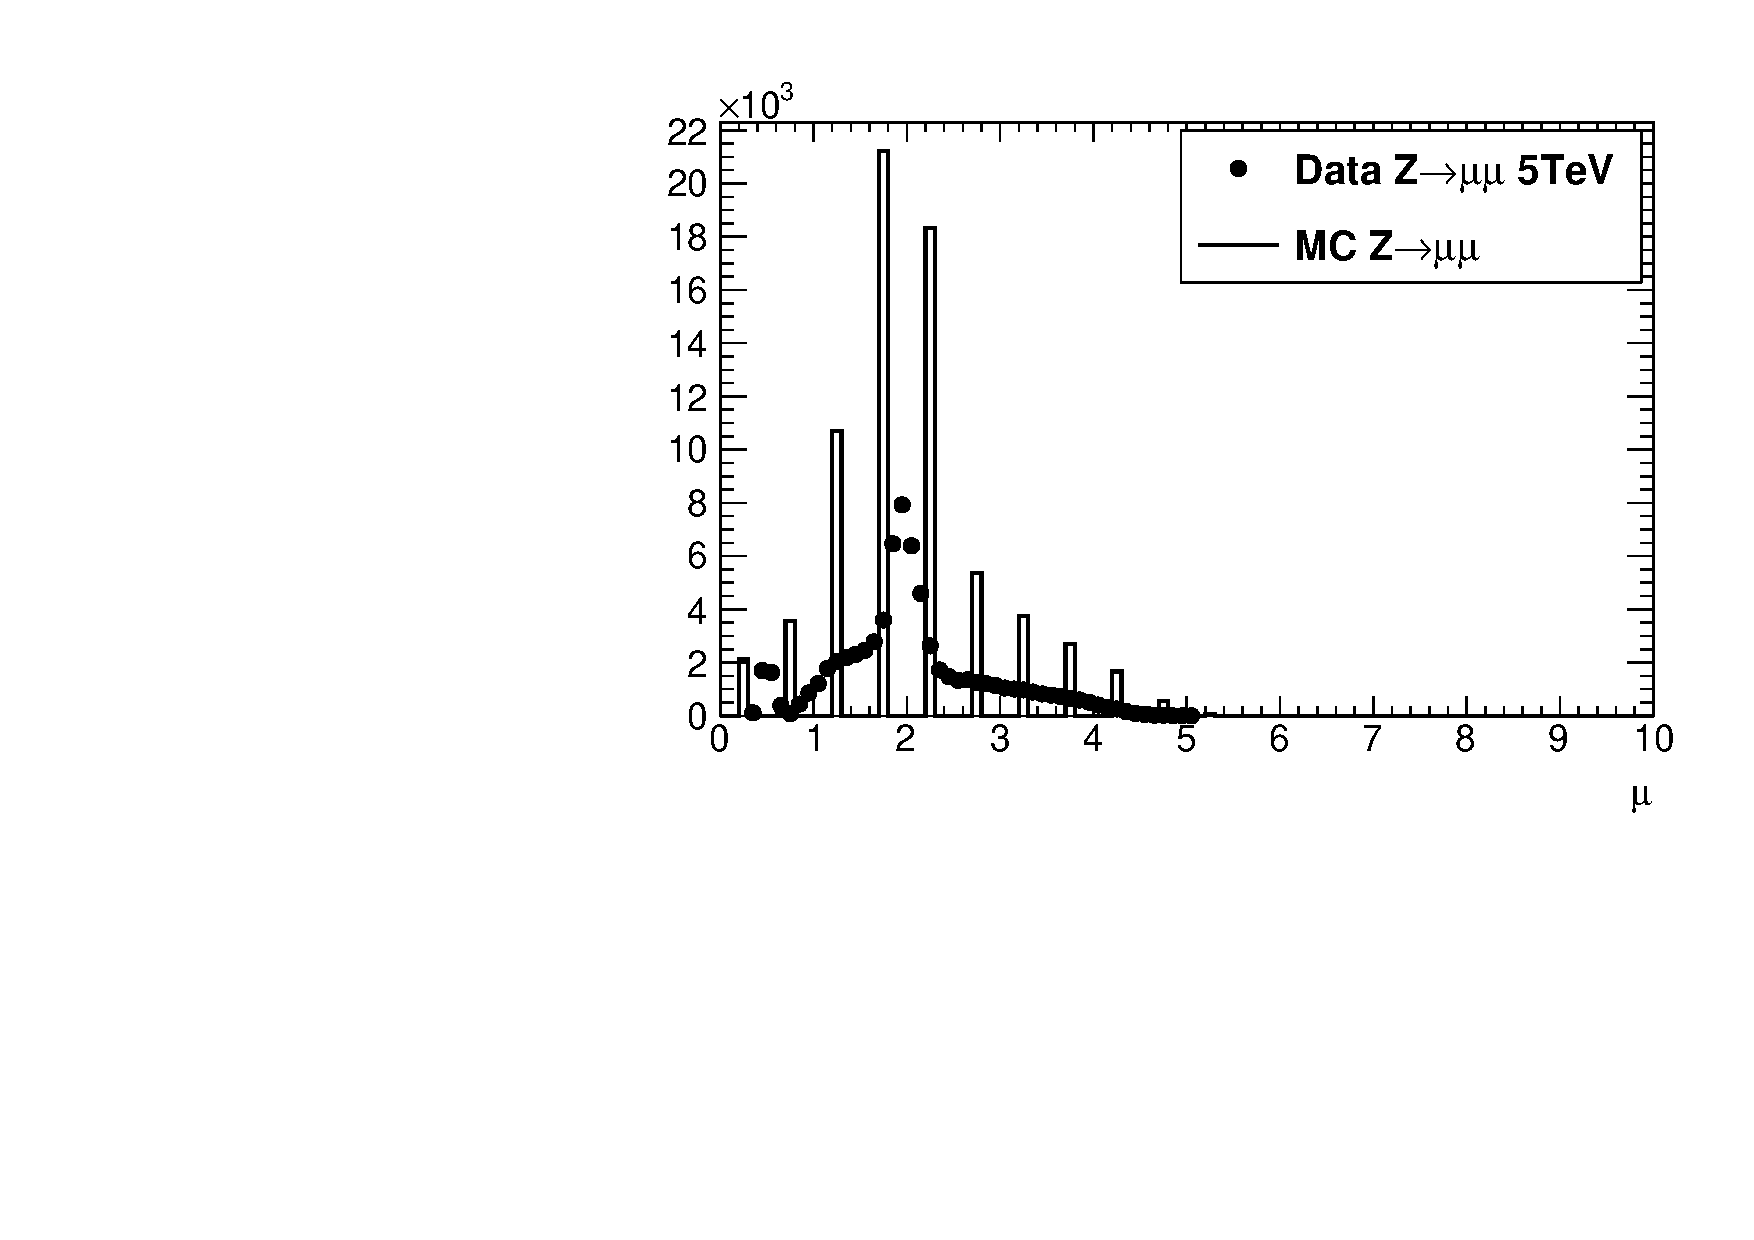
\includegraphics[width=.33\textwidth]{zmumu_5tev_mufine.pdf}%
		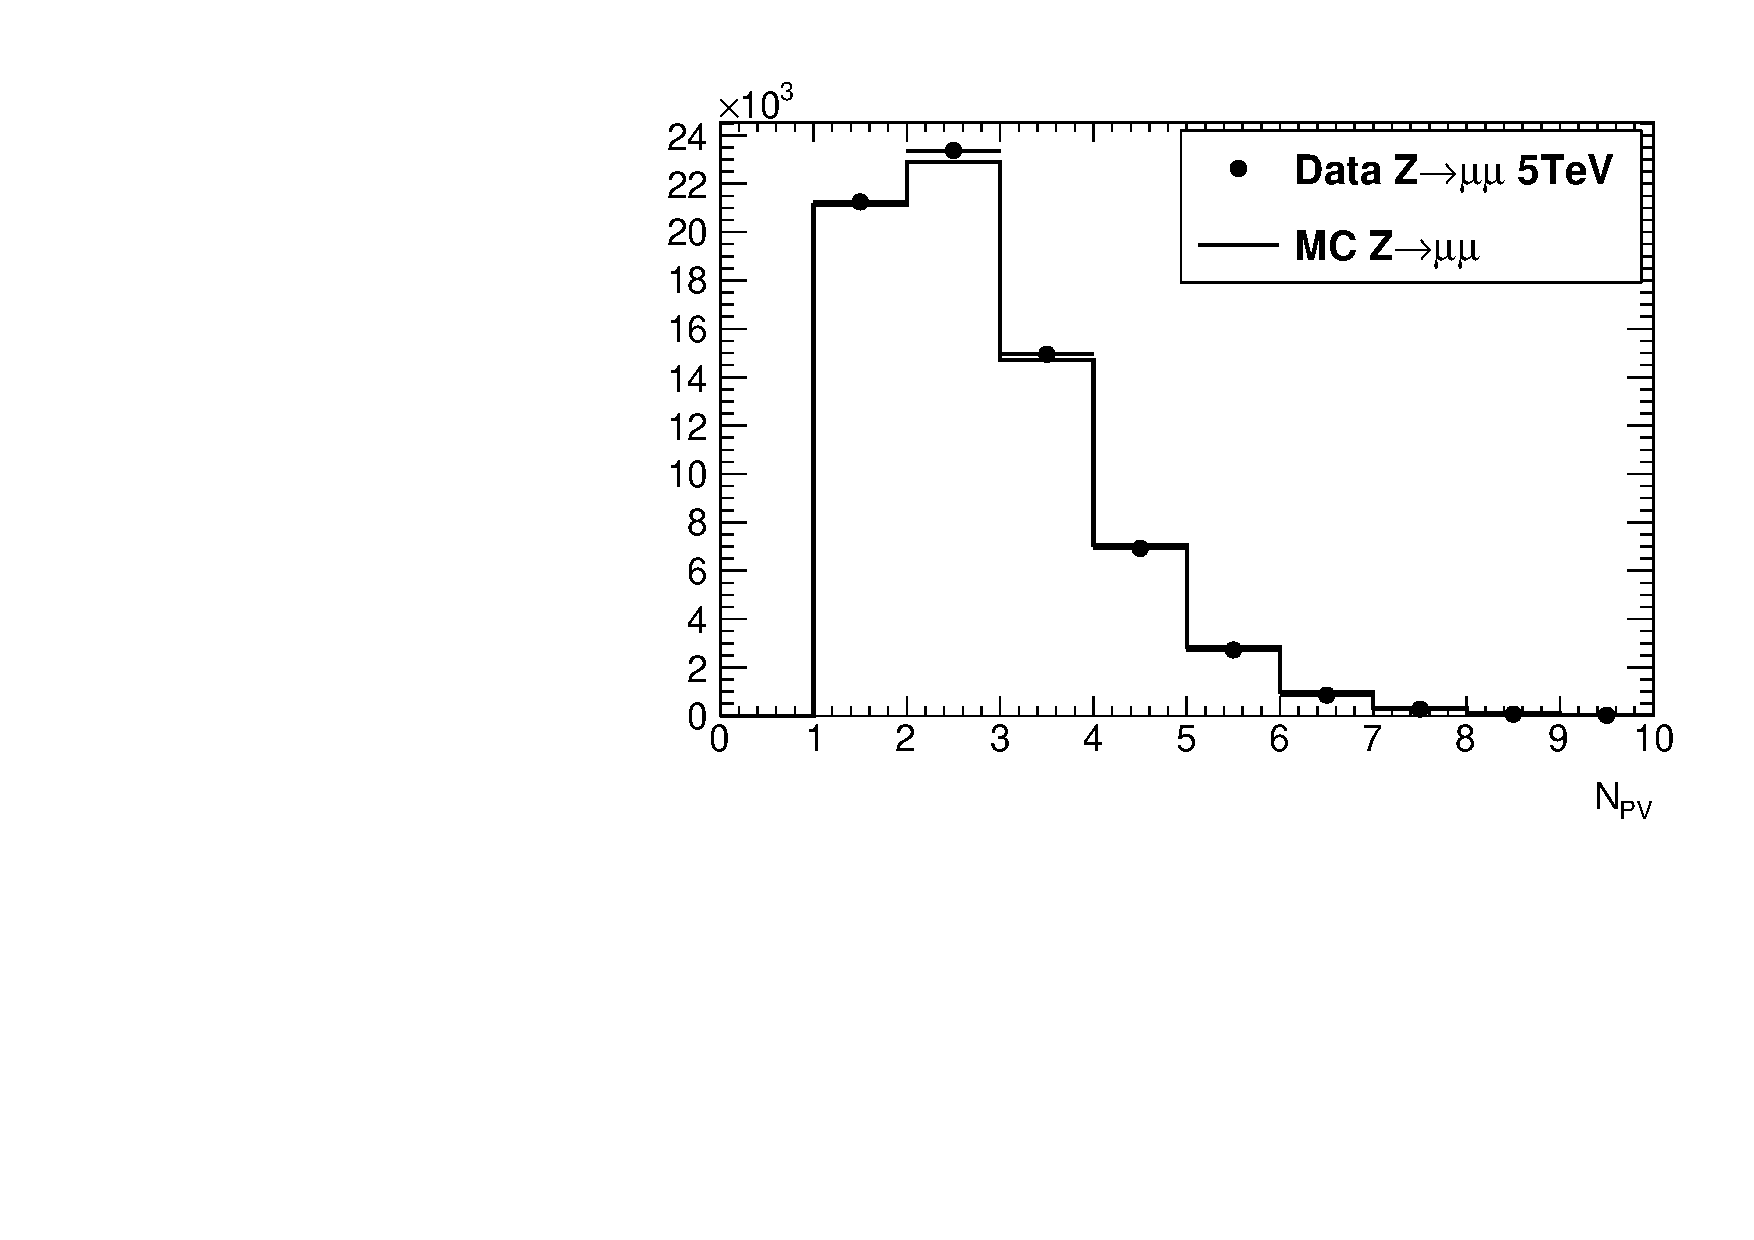
\includegraphics[width=.33\textwidth]{zmumu_5tev_npv.pdf}
		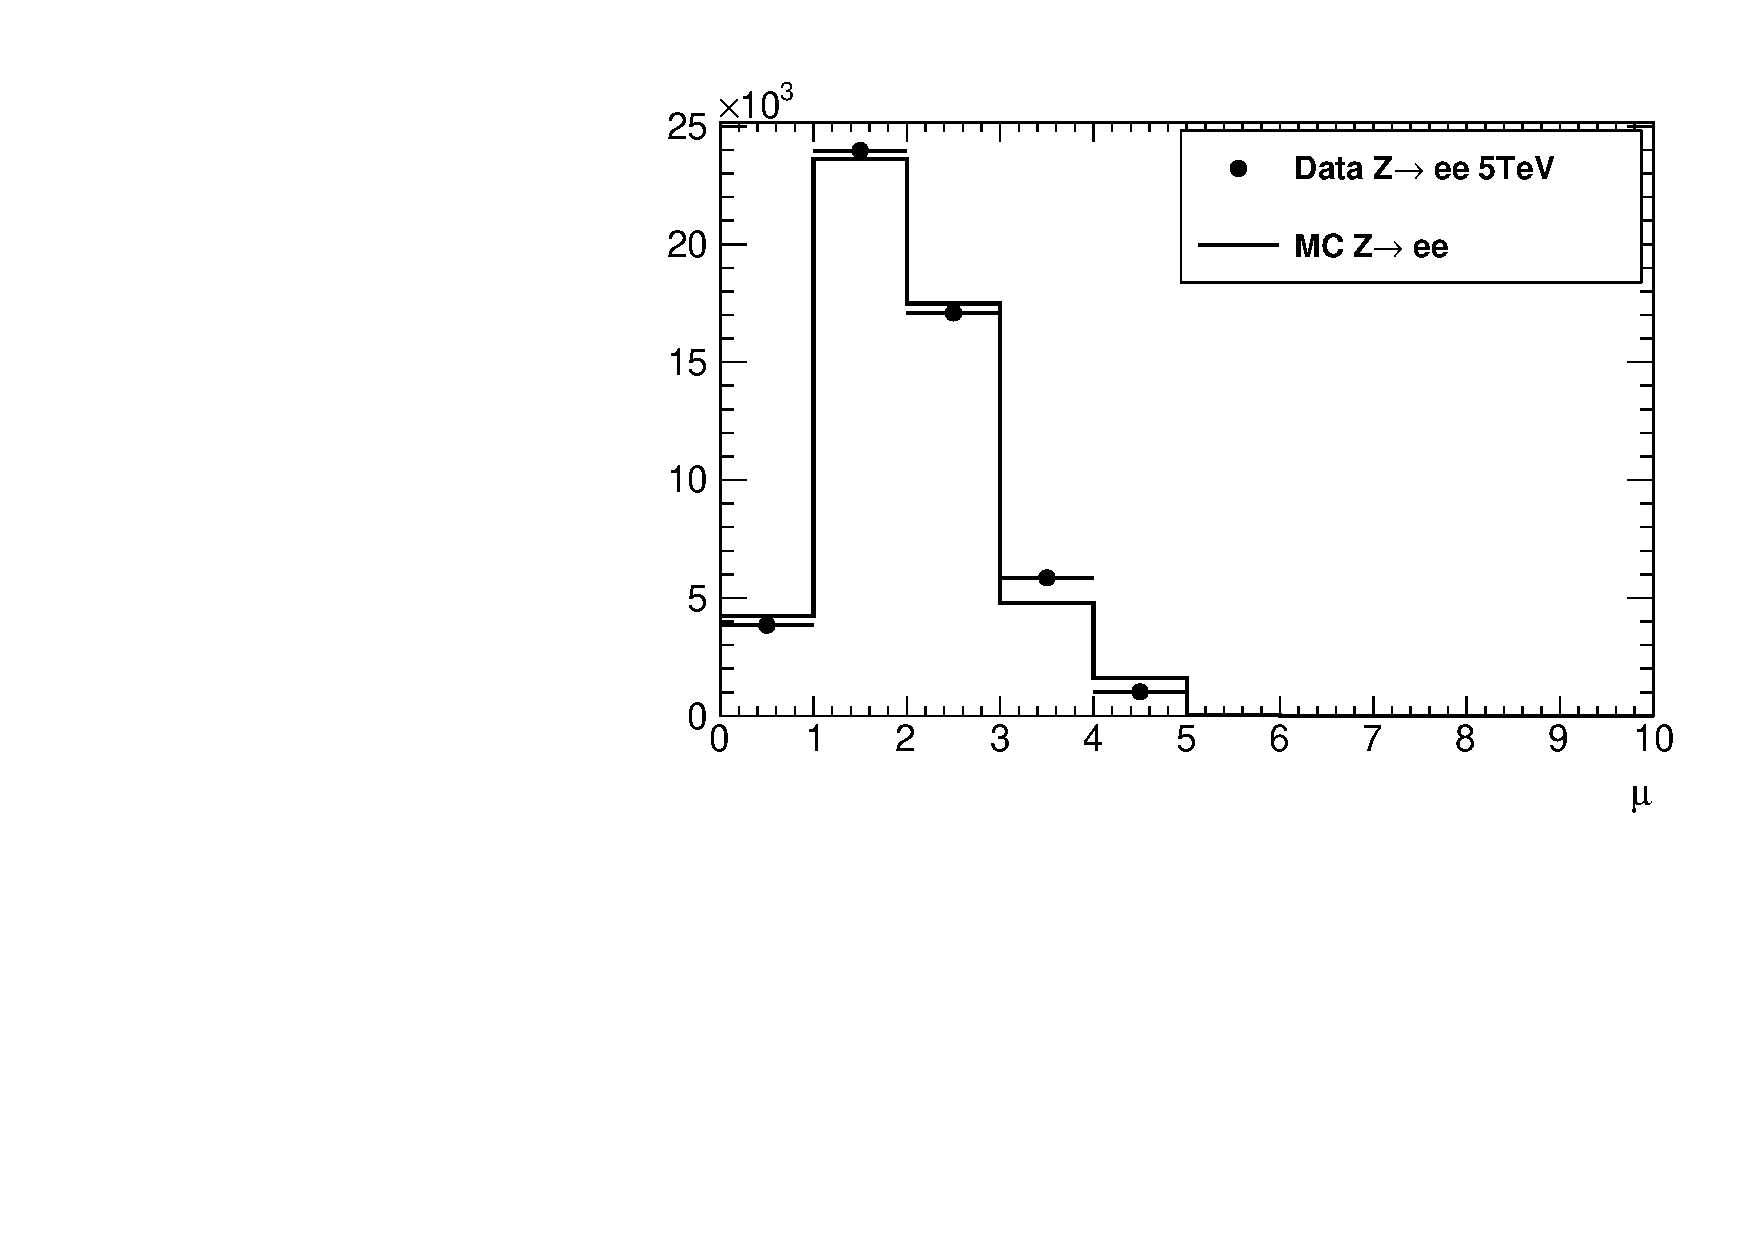
\includegraphics[width=.33\textwidth]{zee_5tev_mu.pdf}%
		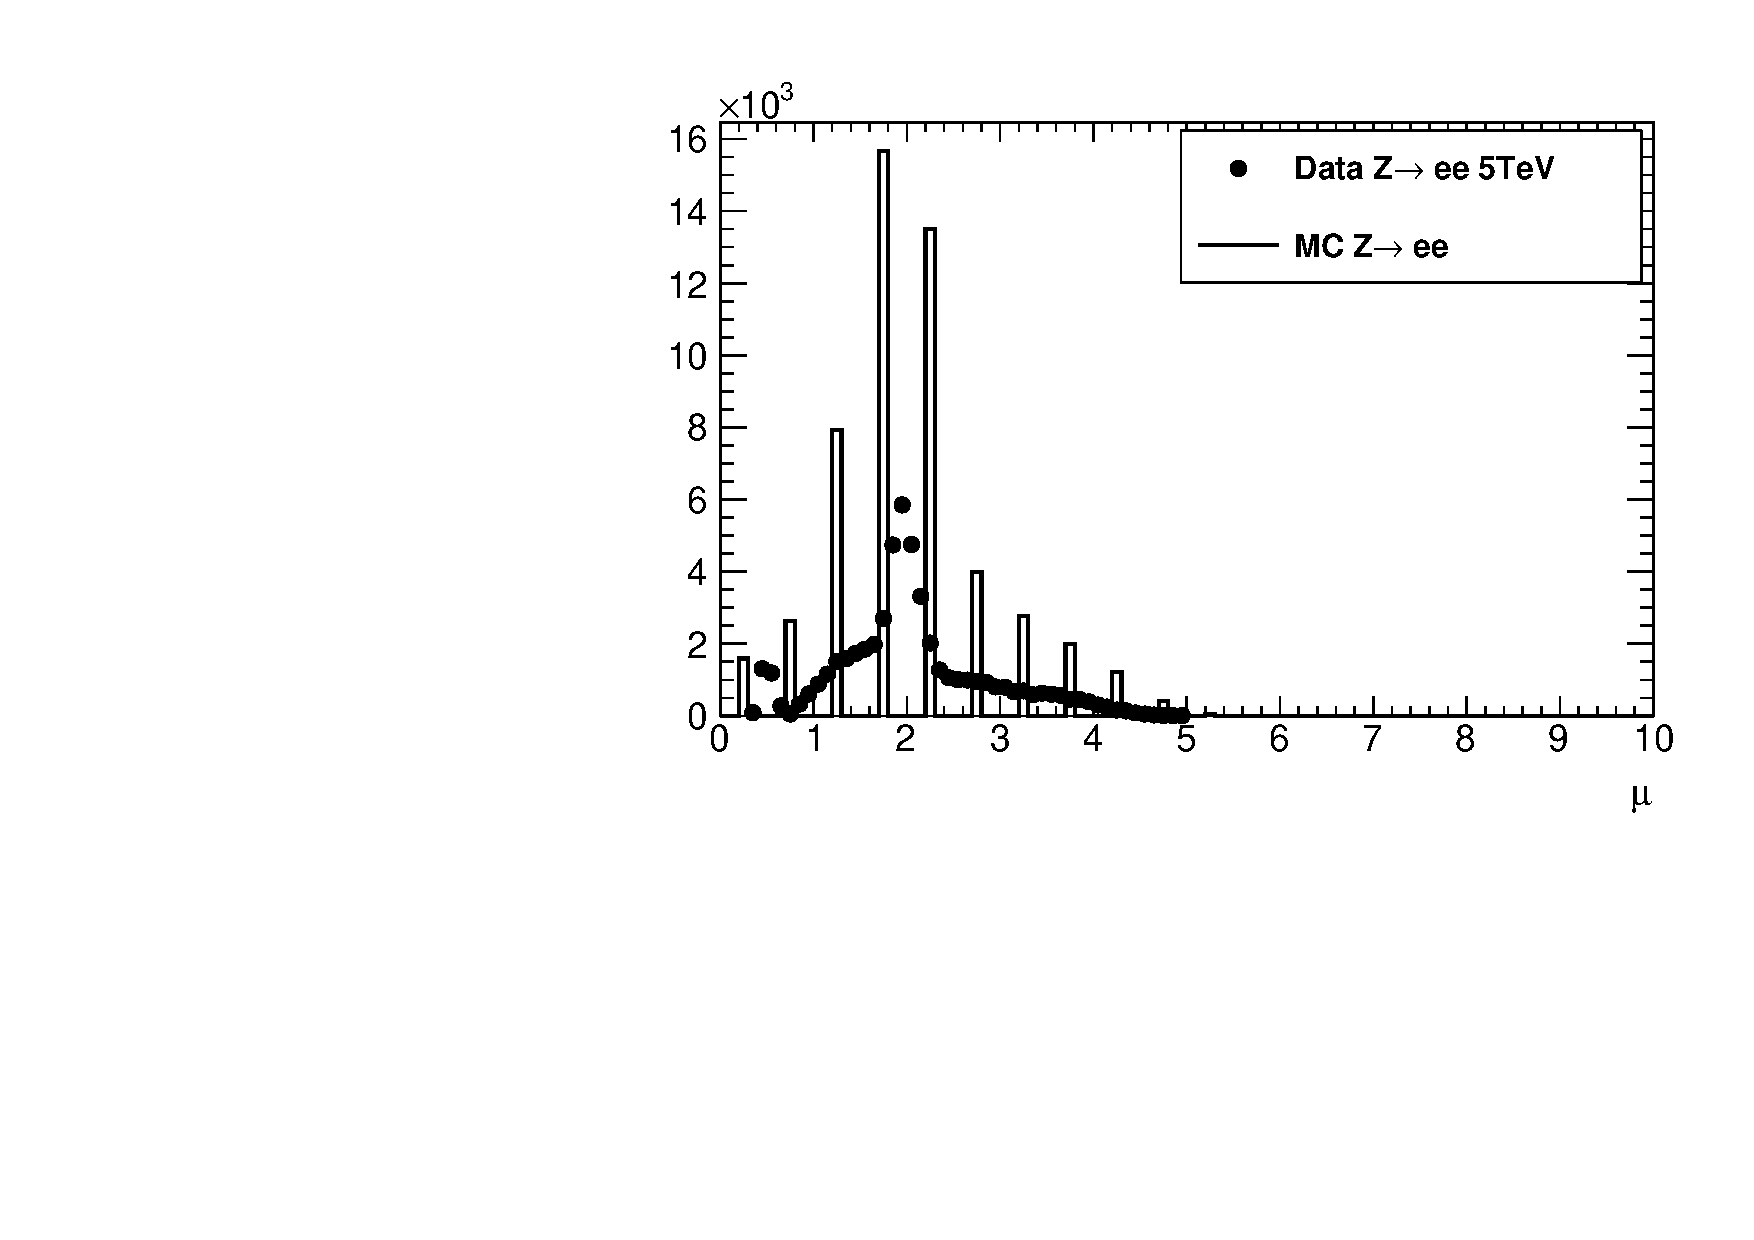
\includegraphics[width=.33\textwidth]{zee_5tev_mufine.pdf}%
		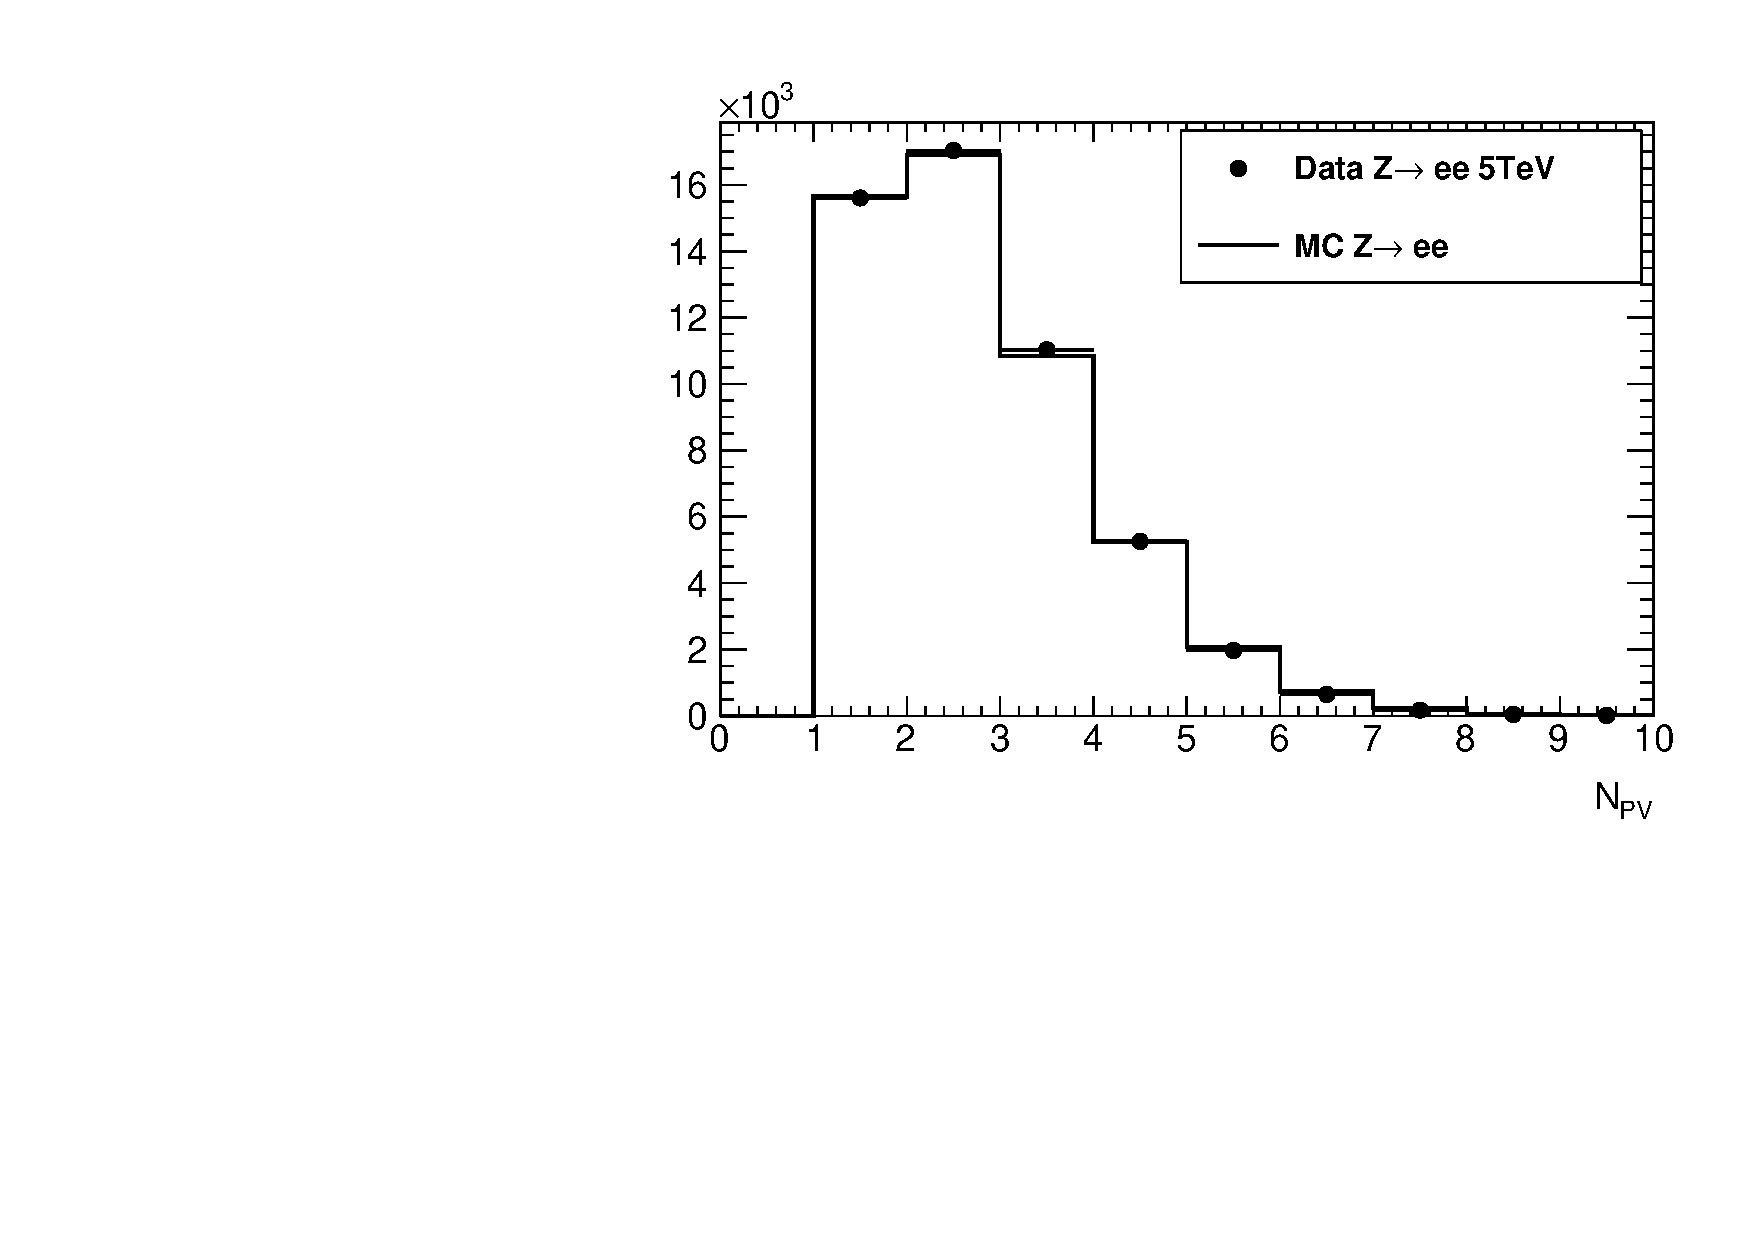
\includegraphics[width=.33\textwidth]{zee_5tev_npv}
		\caption{Distributions for the 5 TeV low-$\mu$ dataset in a $\Zgmm$
			(top row) and a \Zgee (bottom row) selection. The data (points) is
			compared to \Zgmm or \Zgee signal MC, respectively. The left and
			middle plots show the actual $\mu$ in a coarsely-binned and a
			finely-binned version. The right plot shows the number of
			reconstructed primary vertices $N_{PV}$.}
		\label{fig:mu5}
	\end{figure}
	
	\begin{figure}[tph]
		\centering
		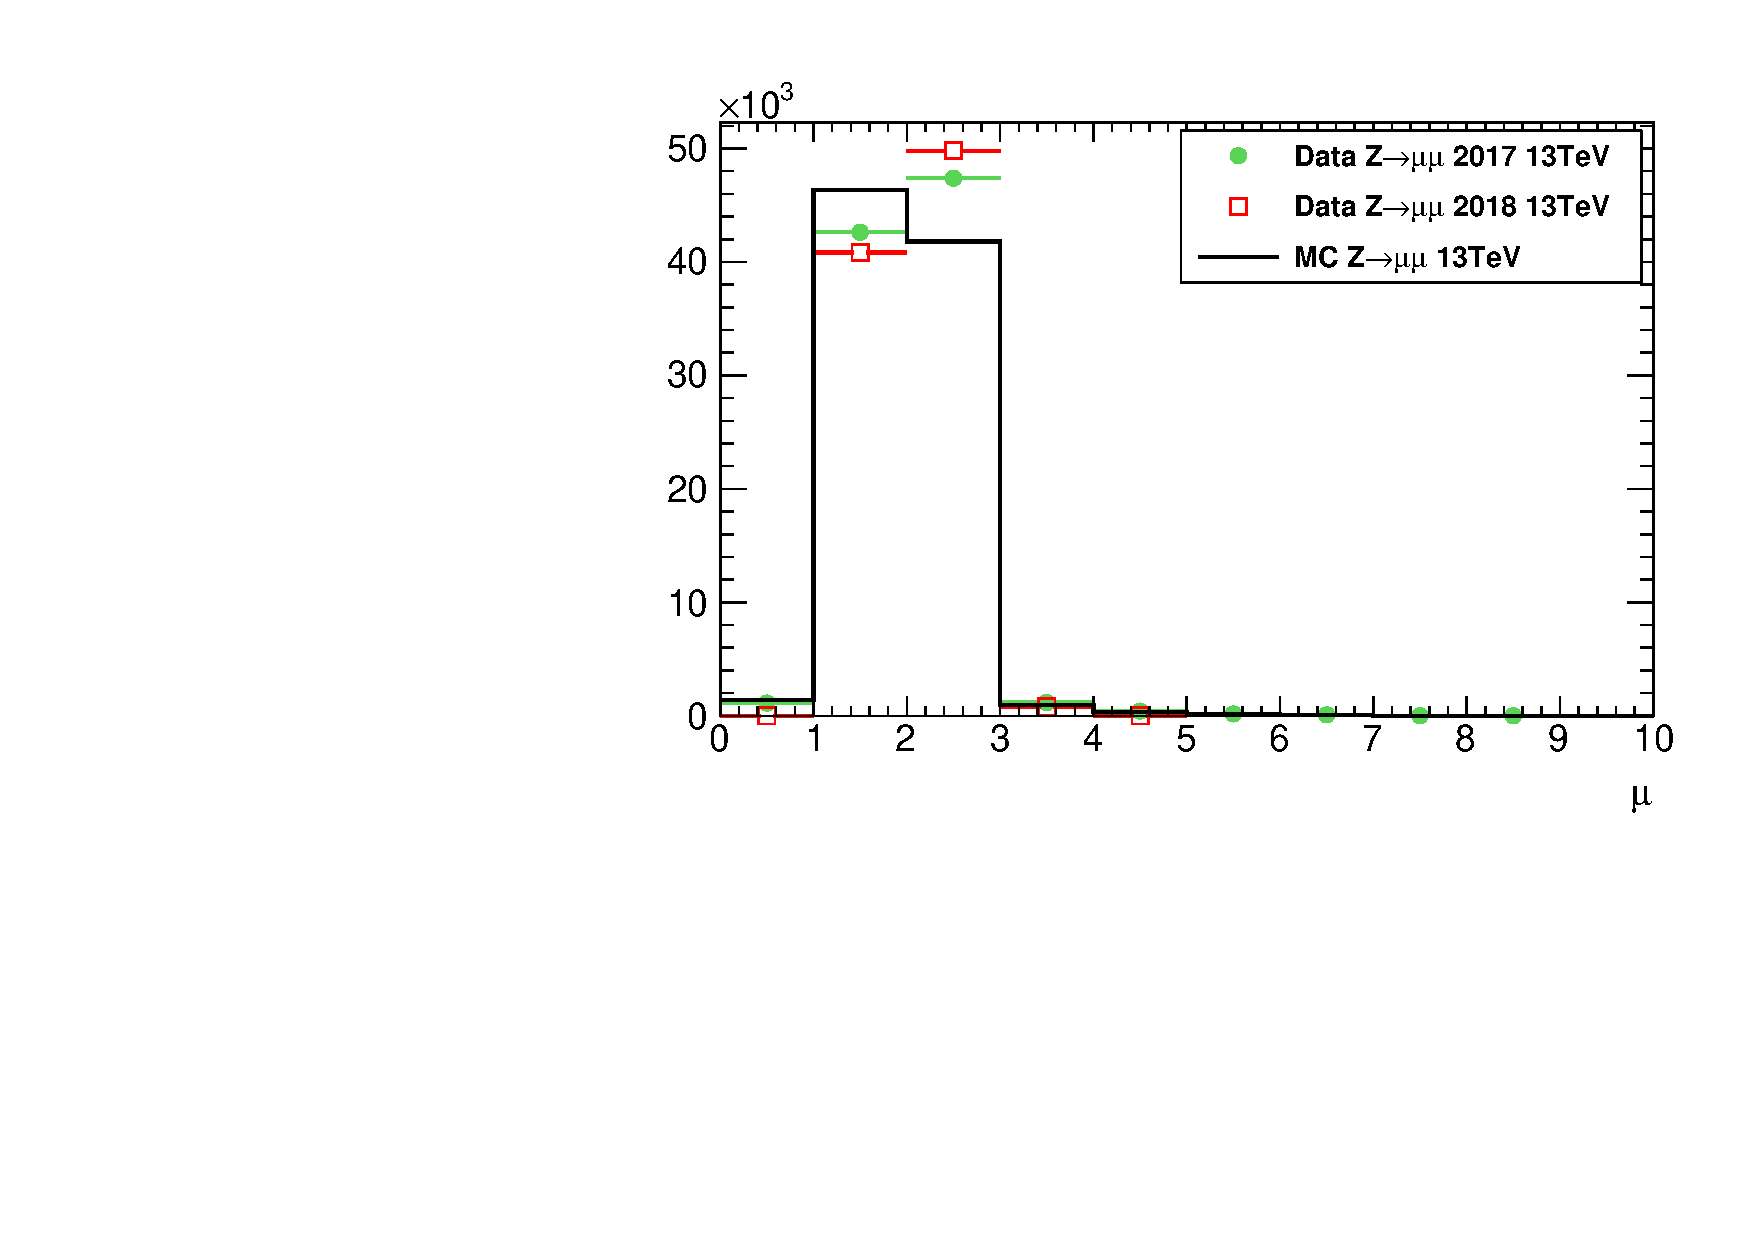
\includegraphics[width=.33\textwidth]{zmumu_13tev_mu}%
		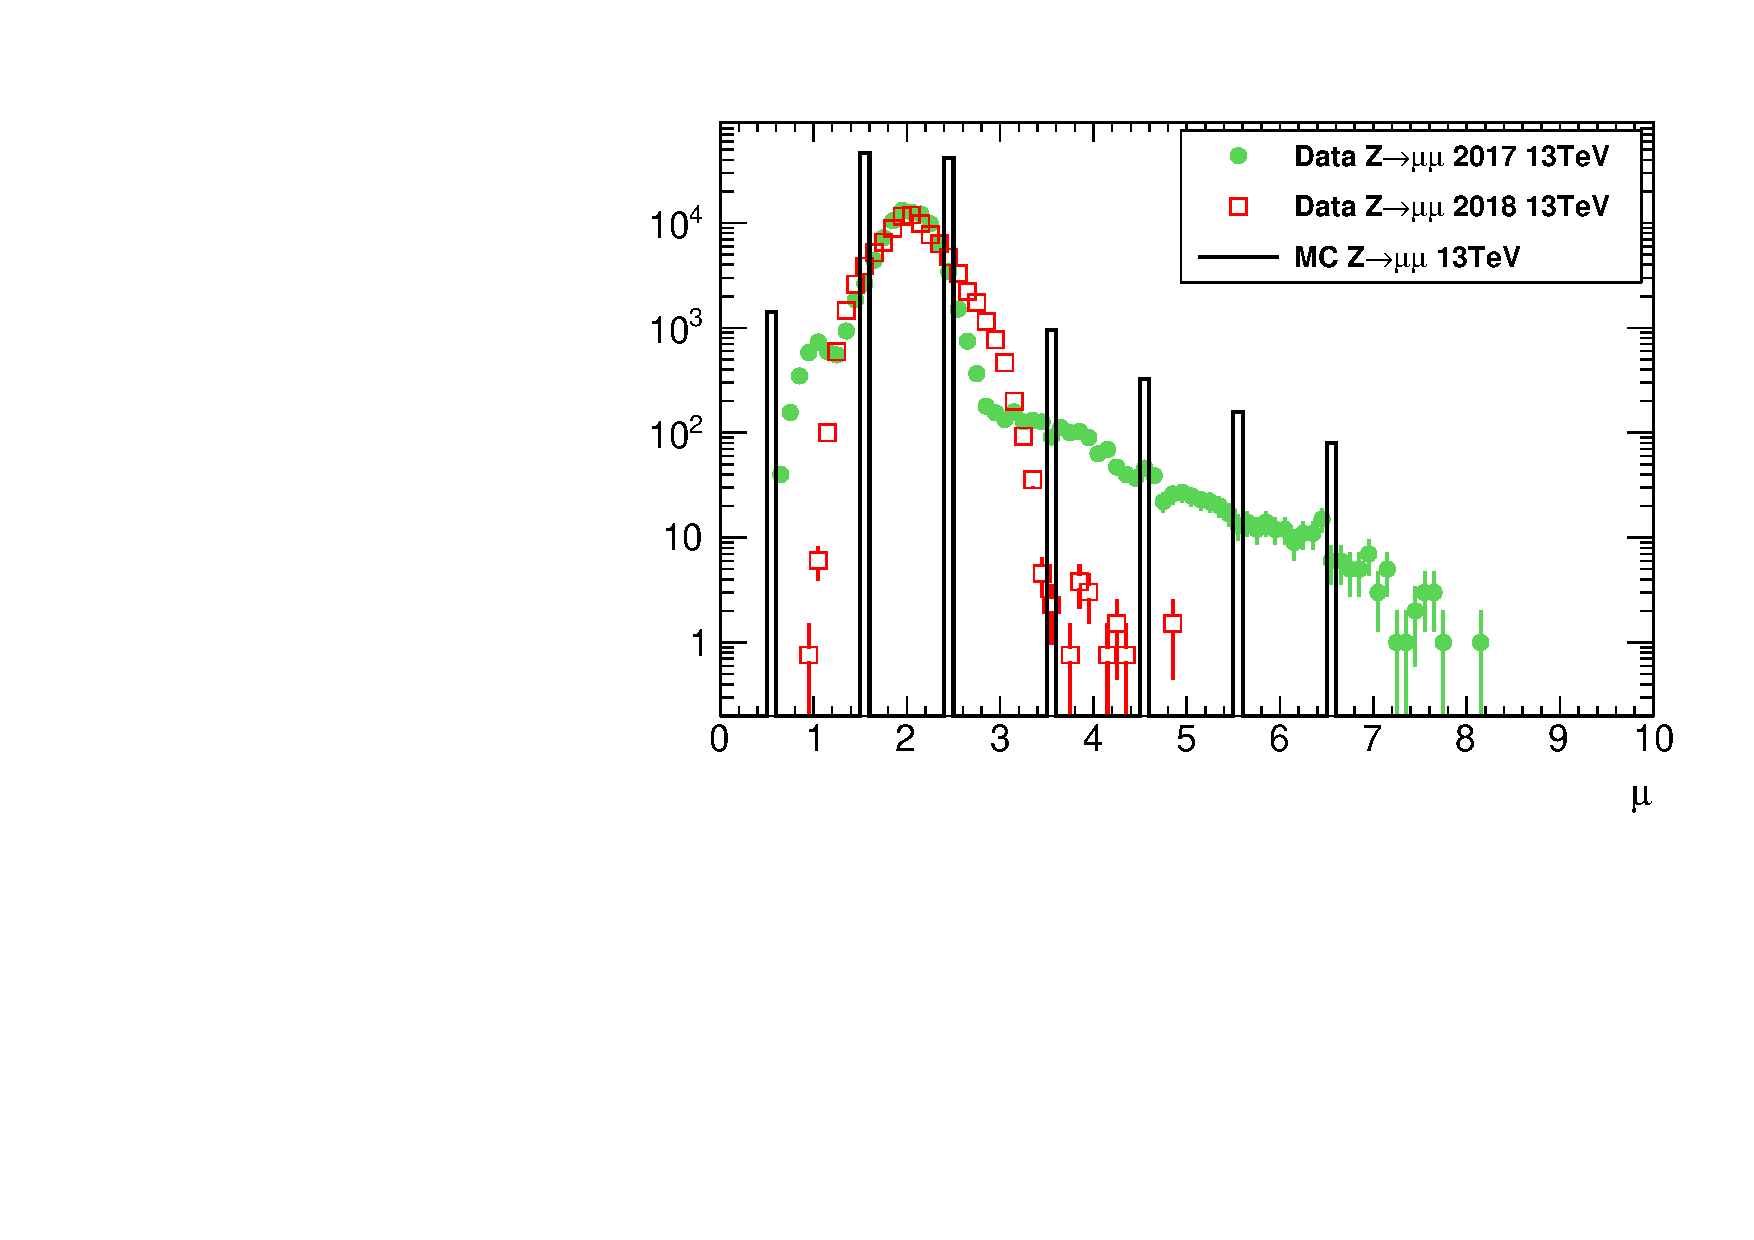
\includegraphics[width=.33\textwidth]{zmumu_13tev_mufine_log}%
		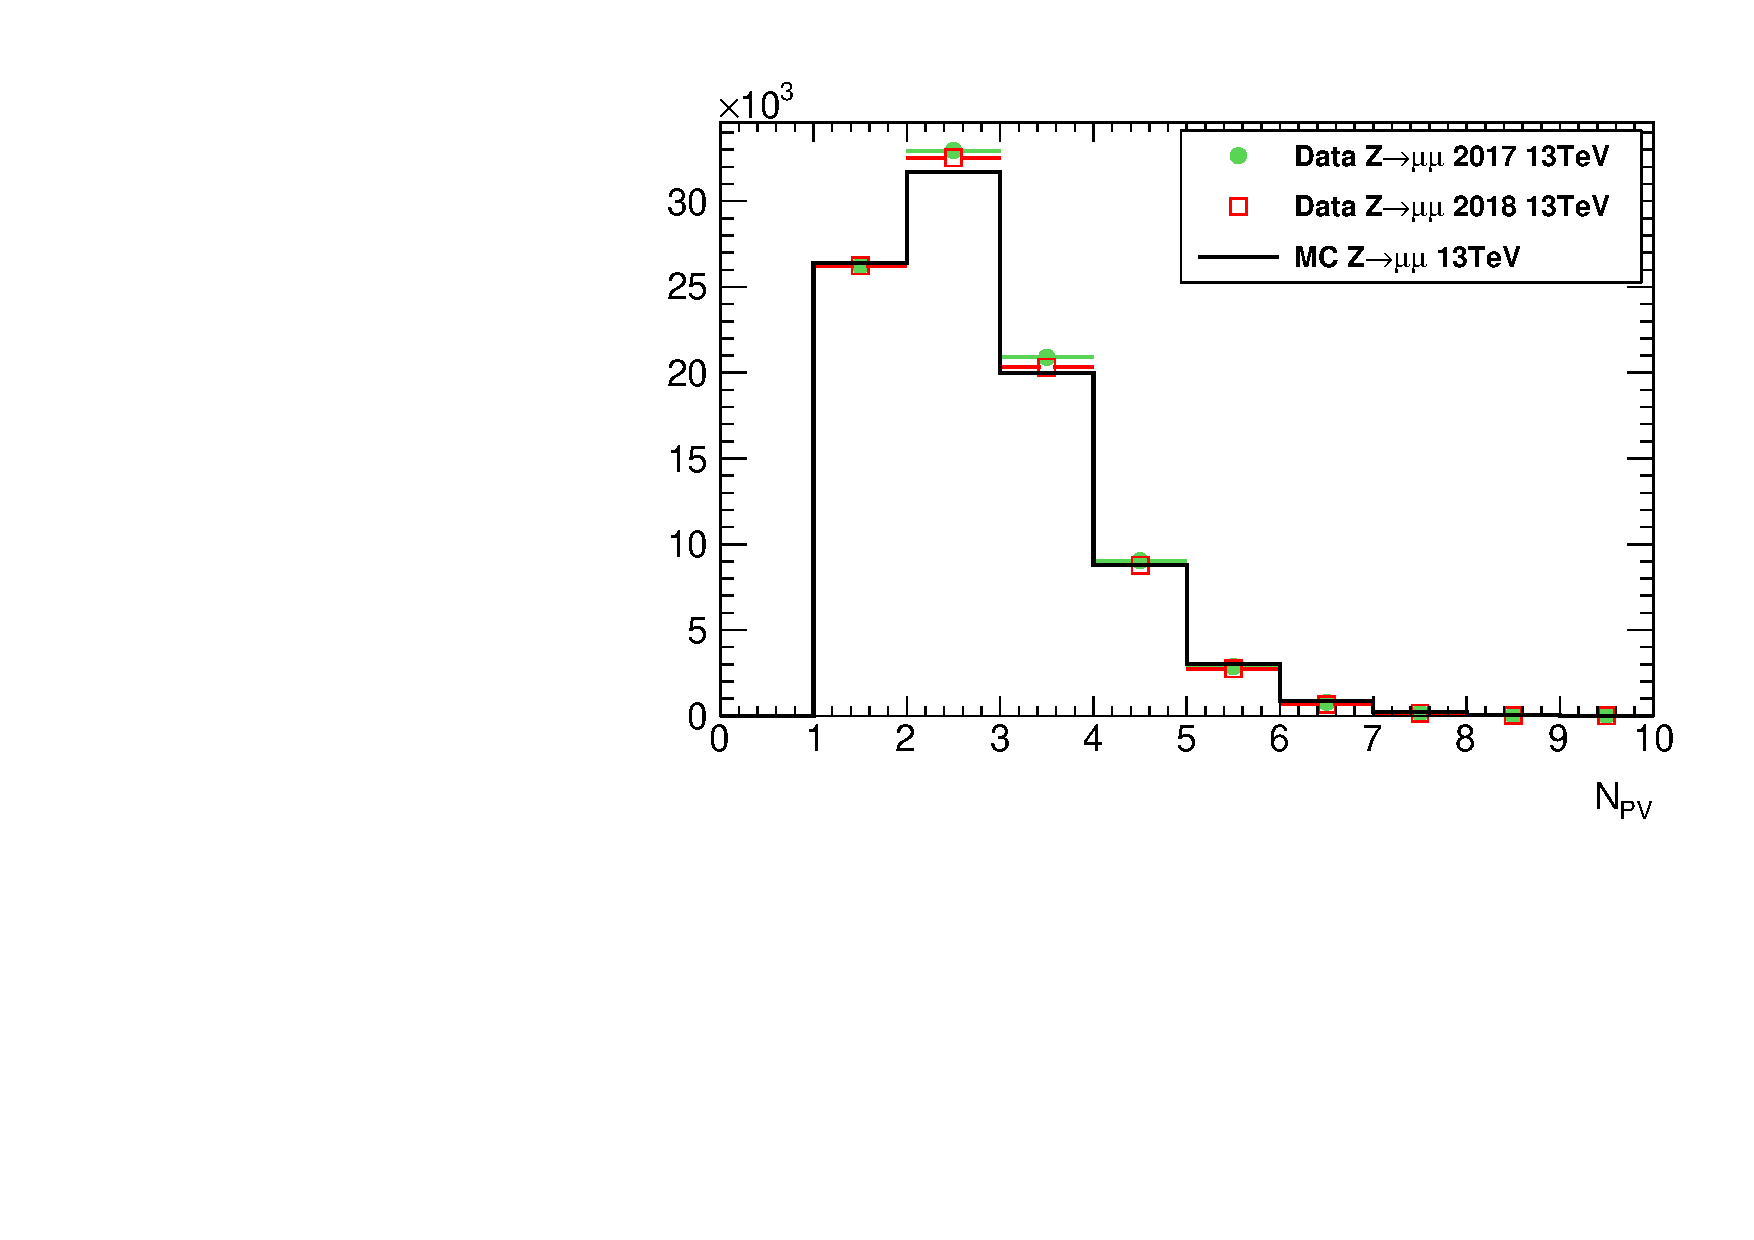
\includegraphics[width=.33\textwidth]{zmumu_13tev_npv}
		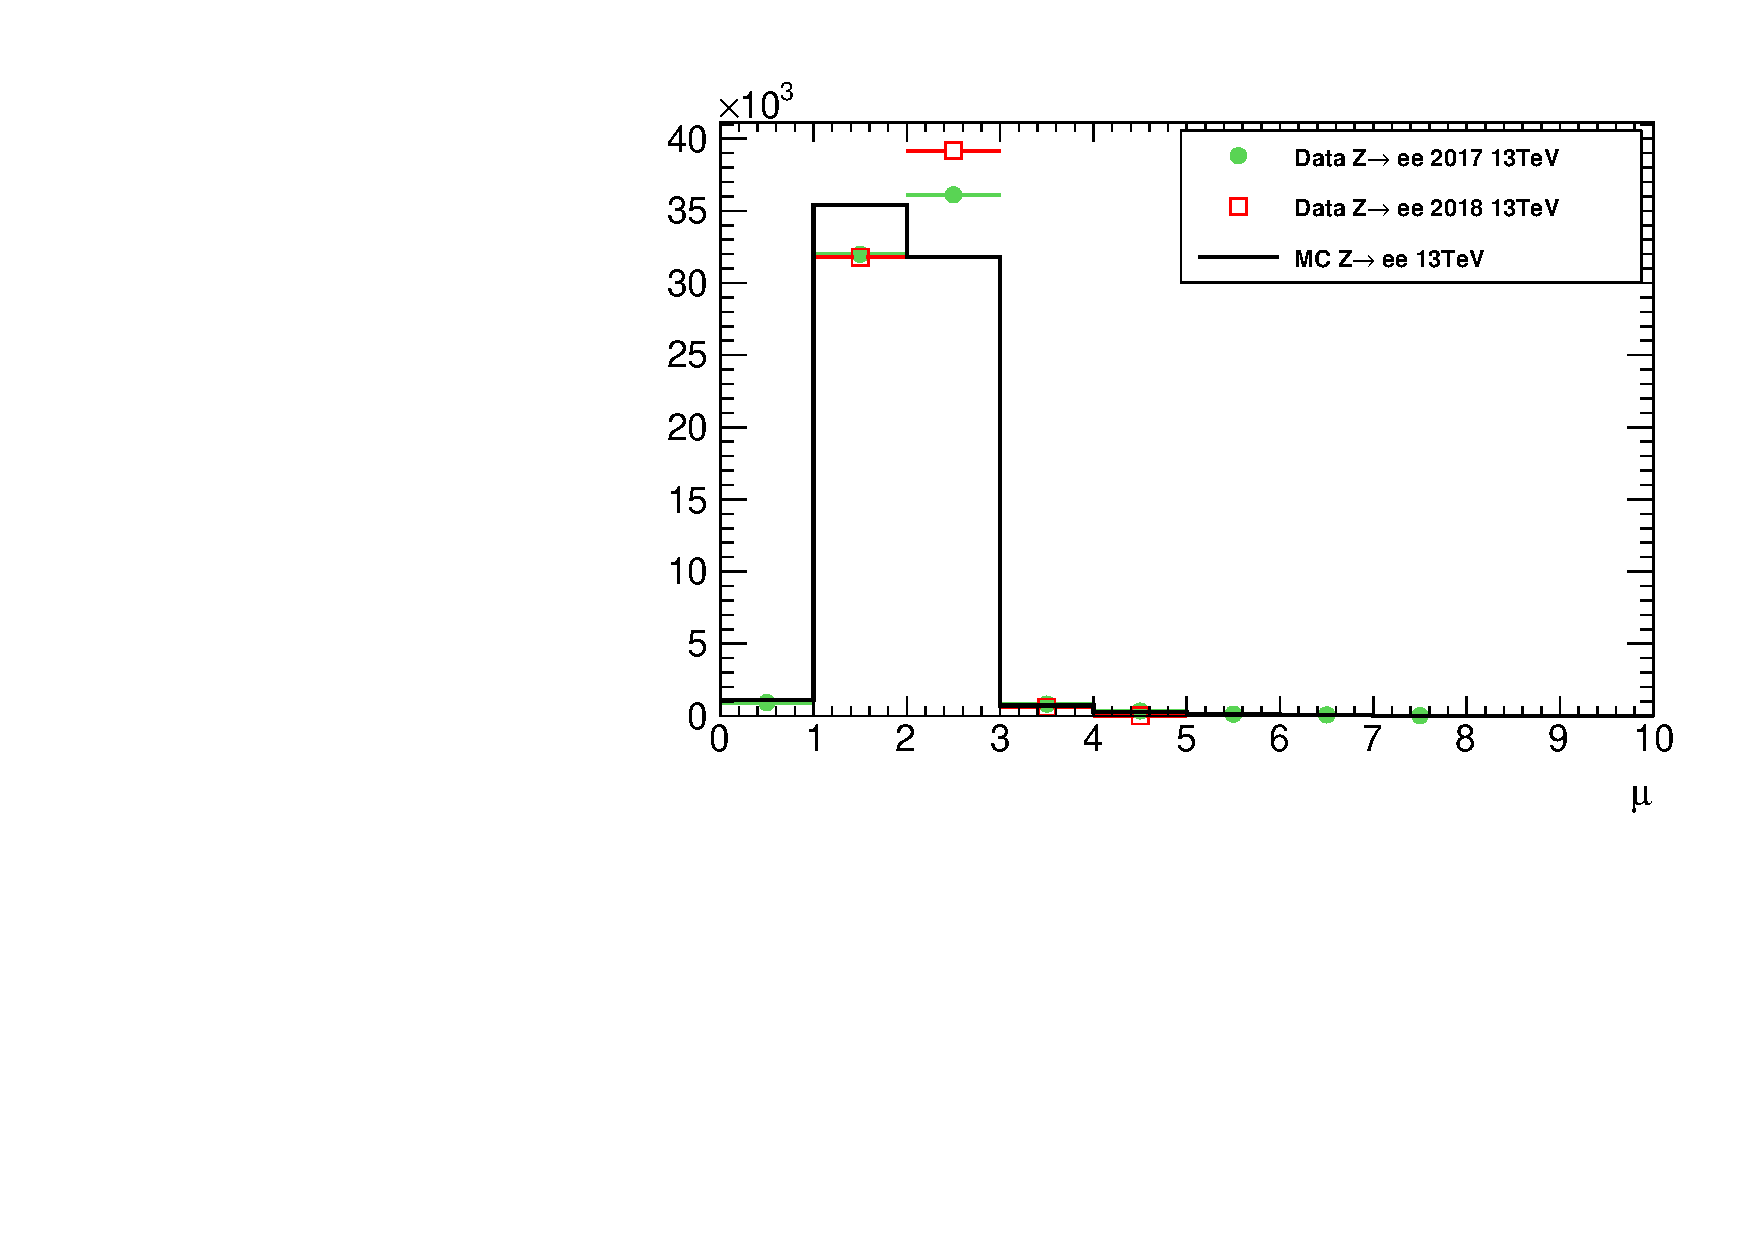
\includegraphics[width=.33\textwidth]{zee_13tev_mu}%
		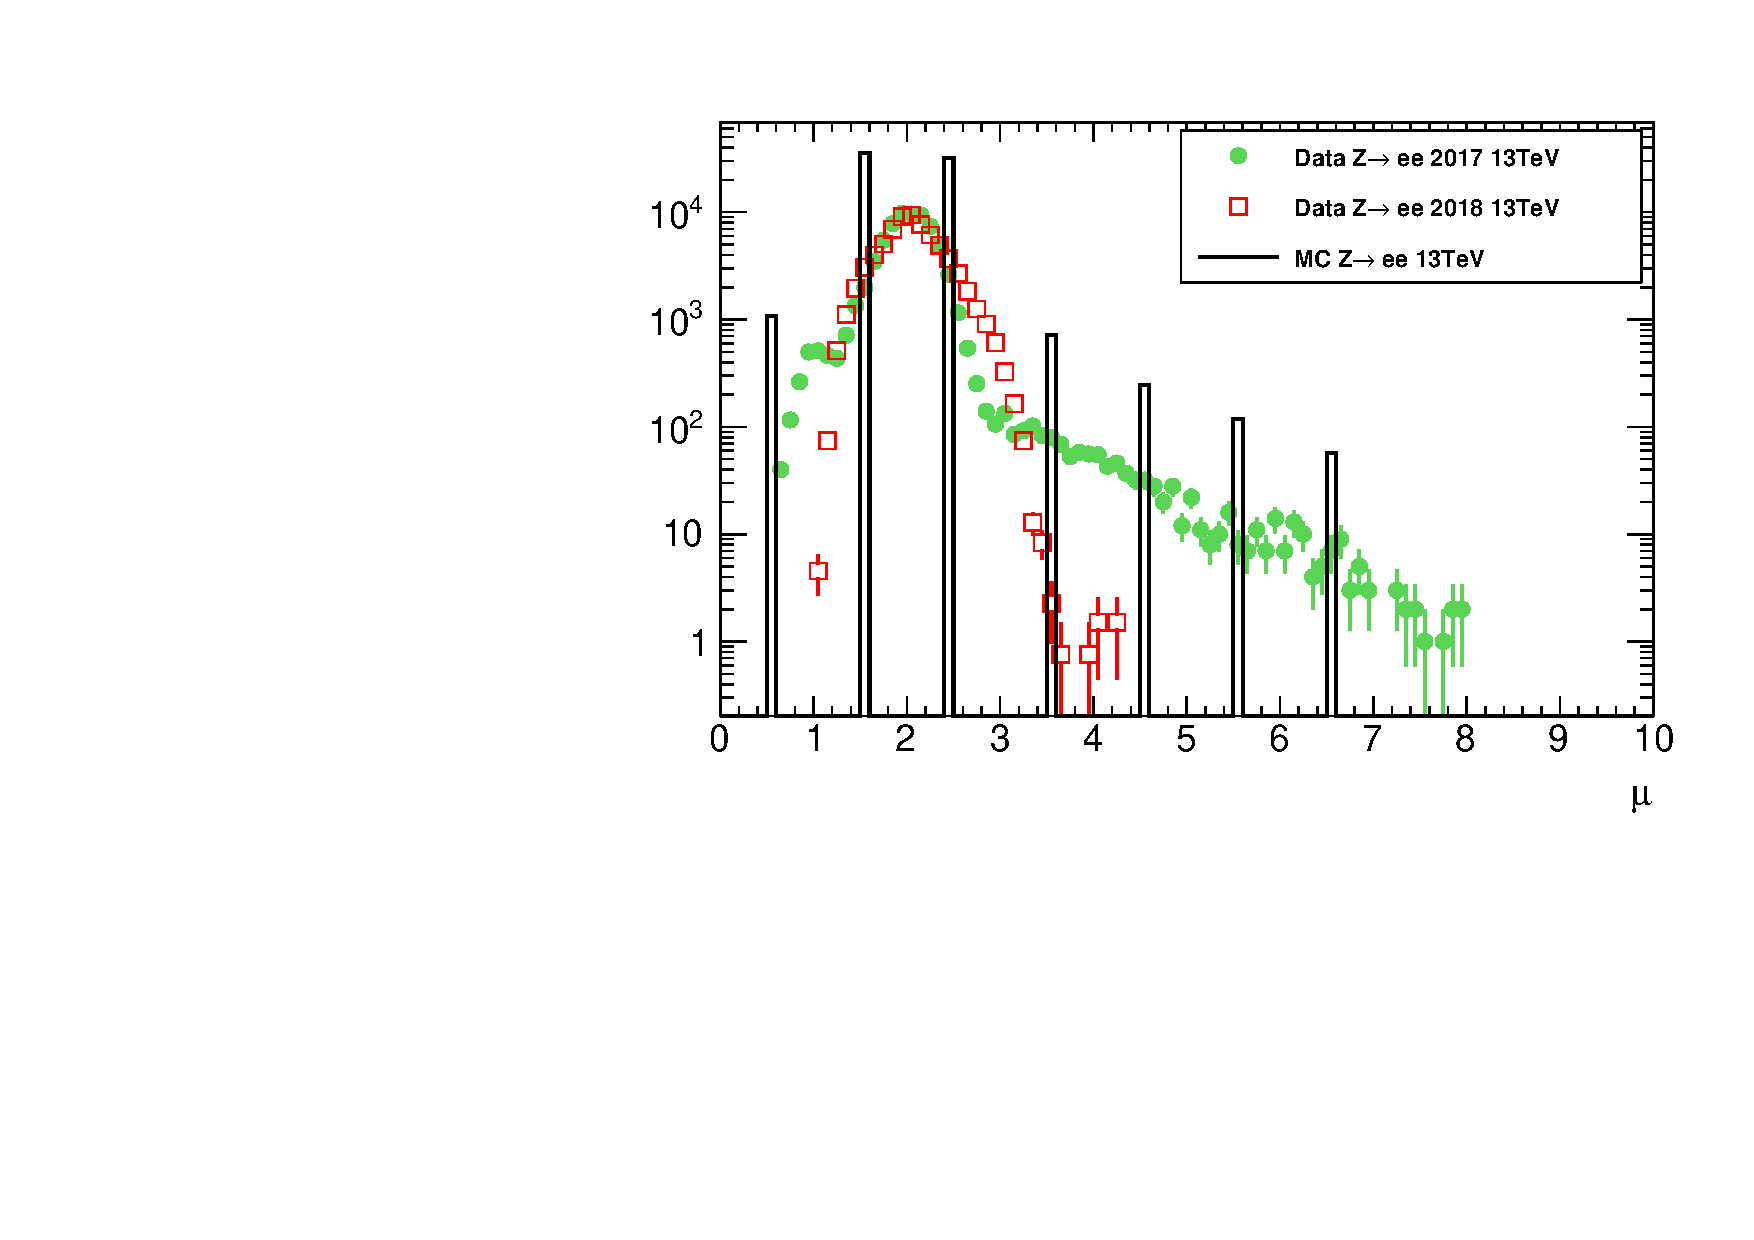
\includegraphics[width=.33\textwidth]{zee_13tev_mufine_log}%
		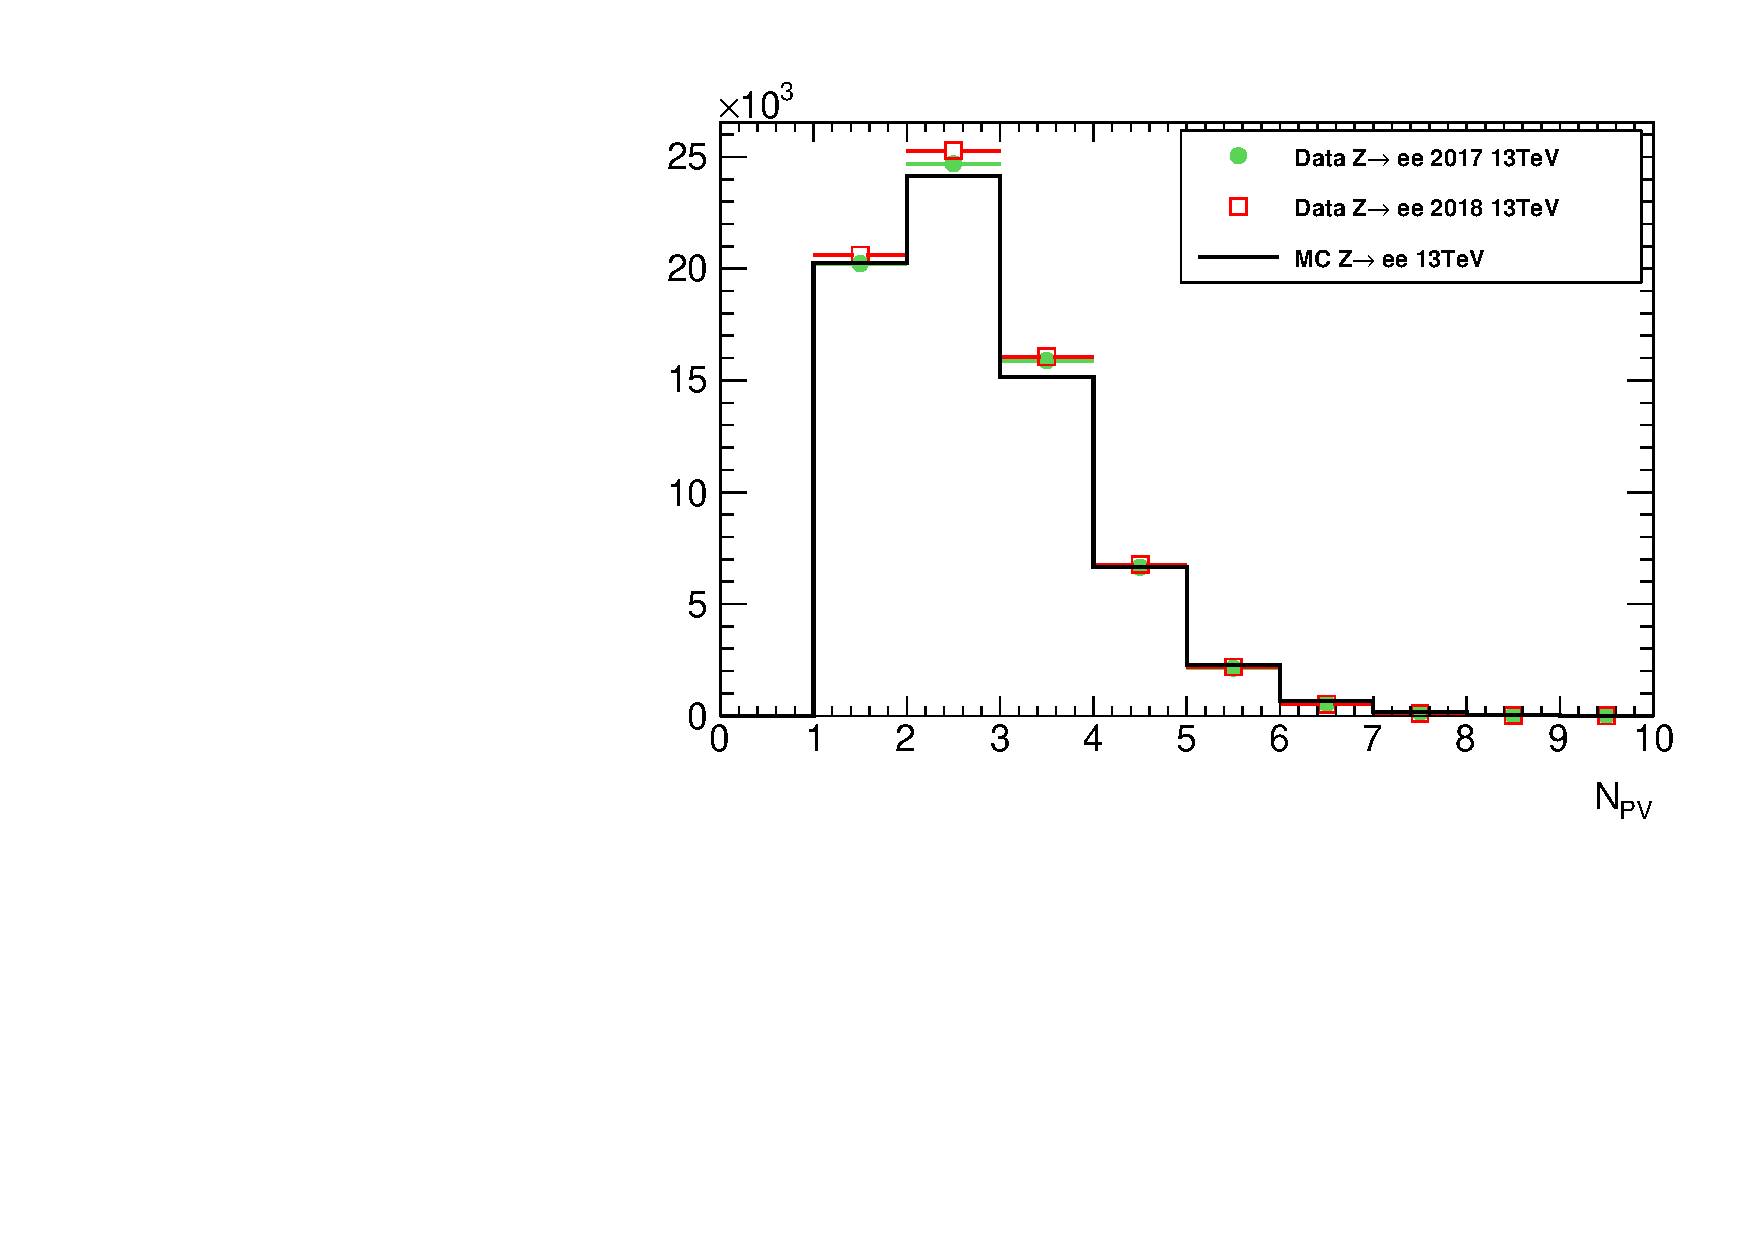
\includegraphics[width=.33\textwidth]{zee_13tev_npv}
		\caption{Distributions for the 13 TeV low-$\mu$ datasets taken in
			2017 and 2018 in a \Zgmm (top row) and a \Zgee (bottom row)
			selection. The data (points) is compared to \Zgmm or \Zgee signal
			MC, respectively. All distributions are (roughly) normalised to
			the same number of selected events in the 2017 dataset. The left
			and middle plots show the actual $\mu$ in a coarsely-binned and a
			finely-binned version. The right plot shows the number of
			reconstructed primary vertices $N_{PV}$.}
		\label{fig:mu13}
	\end{figure}
	
    \subsection{MC samples and cross-sections}
    Signal and background processes are modelled using fully simulated and reconstructed using \gls{mc} samples, specifically tuned for the special run conditions, namely the pileup conditions, lower topo-cluster noise thresholds and adapter trigger menu. No pileup reweighting is performed.\\
    The information on the simulated samples and their properties is given in Tables \ref{tab:samples13}, \ref{tab:samples13_sherpaz}, \ref{tab:samples13_sherpaw},  \ref{tab:samples5} \cite{Kretzschmar:2657141}. The predicted event counts are normalized to the cross-sections quoted in the table.\\
    The primary signal event samples for W and Z production are obtained using \Powheg~\cite{Nason:2004rx,Frixione:2007vw,Alioli:2008gx,Alioli:2010xd} event generator with CT10 PDF, linked with \Pythia~\cite{pythia} with AZNLO tune~\cite{STDM-2012-23}. \Powheg+\Pythia8 samples are interfaced to \Photos~\cite{Golonka:2005pn}  for final state \gls{qed} effects simulation.\\
    A set of alternative samples at $\sqrt{s} = 13\tev$ was prepared with \Sherpa 2.2.2~\cite{Hoche:2010kg} using the NNPDF3.0 PDFs and merging
    $V+0,1,2$ at NLO accuracy with $V+3,4$ at LO accuracy with the MEPS@NLO scheme. A similar set for $\sqrt{s} = 5\tev$ was prepared with \Sherpa 2.2.5 with a setup similar to 13 TeV samples.\\
    Pileup is modelled by overlaying simulated soft events over the original hard-scattering event. These soft events were modelled using \Pythia\ with NNPDF2.3LO set of PDFs~\cite{Ball:2012cx} and the A3 tune~\cite{ATL-PHYS-PUB-2016-017}.\\
    The $W$ and $Z$ processes samples are normalized to NNLO
    calculations performed using the DYTURBO, an optimised version
    of DYNNLO~\cite{Catani:2007vq,Catani:2009sm} using the MMHT2014nnlo PDF
    set~\cite{Harland-Lang:2014zoa}. Corresponding numerical values were taken from
    the corresponding ATLAS publications of the 2015 data at 13
    TeV~\cite{STDM-2015-03} and 5.02 TeV~\cite{HION-2018-02} are presented in Table~\ref{tab:samples13} for 13 TeV and Table~\ref{tab:samples5} for 5 TeV. The
    uncertainties on those cross-sections arise from the choice of PDF set, from factorization
    and renormalisation scale dependence, and the strong
    coupling constant $\alpha_s$ uncertainty resulting in the total 
    uncertainty estimate of $5\%$.
    
    Backgrounds from top-quark pair-production $t\bar{t}$ and 
    single-top production ($Wt$, t-channel, s-channel) were generated with
    \Powheg+\Pythia.
    The 5 TeV $t\bar{t}$ cross section is taken as the top++ prediction observed by CMS~\cite{CMS-TOP-16-023}.
    Di-boson combinations $VV, V=W,Z$ are generated with \Sherpa\ in all decay channels with a requirement of having at least one real lepton in the final state.
    
    \begin{table}[htbp]
    	\begin{center}
    		\begin{tabular}{l|l|l|l|l|l}
    			\hline
    			\hline
    			Process & Data set & Generator& $\sigma{\cdot}
    			\text{BR}{\cdot}\epsilon_\mathrm{filter}$ [nb] (th. unc.)
    			& $N^\mathrm{skim}_\mathrm{evt}\,[10^6]$
    			& $N^\mathrm{unskim}_\mathrm{evt}\,[10^6]$\\
    			\hline\hline
    			$ W^{+} \to e^{+}\nu $ & 361100 & \Powheg+\Pythia & 11.61 (5\%)  & 40 & 40 \\\hline
    			$ W^{+} \to \mu^{+}\nu $ & 361101 & \Powheg+\Pythia & 11.61 (5\%)  & 40 & 40 \\\hline
    			$ W^{+} \to \tau^{+}\nu $ & 361102 & \Powheg+\Pythia & 11.61 (5\%)  & 0.28 & 5.0 \\\hline
    			$ W^{-} \to e^{-}\bar{\nu} $ & 361103 & \Powheg+\Pythia & 8.630 (5\%)  & 30 & 30 \\\hline
    			$ W^{-} \to \mu^{-}\bar{\nu} $ & 361104 & \Powheg+\Pythia & 8.630 (5\%)  & 29 & 29 \\\hline
    			$ W^{-} \to \tau^{-}\bar{\nu} $ & 361105 & \Powheg+\Pythia & 8.630 (5\%)  & 0.24 & 4.0 \\\hline\hline
    			$ Z \to ee $ & 361106 & \Powheg+\Pythia & 1.910 $\times$ 1.03 (5\%)  & 10 & 10 \\\hline
    			$ Z \to \mu\mu $ & 361107 & \Powheg+\Pythia & 1.910 $\times$ 1.025 (5\%)  & 10 & 10 \\\hline
    			$ Z \to \tau\tau $ & 361108 & \Powheg+\Pythia & 1.910 $\times$ 1.025 (5\%)  & 0.12 & 1.0 \\\hline\hline
    			$ ZZ (q\bar{q}\ell\ell) $ & 363356 & \Sherpa\ 2.2.1 & 0.01556 $\times$ 0.141 (10\%)  & 0.0064 & 0.010 \\\hline
    			$ WZ (q\bar{q}\ell\ell) $ & 363358 & \Sherpa\ 2.2.1 & 0.003433 (10\%)  & 0.0063 & 0.010 \\\hline
    			$ WW (q\bar{q}\ell\nu) $ & 363359 & \Sherpa\ 2.2.1 & 0.02472 (10\%)  & 0.0093 & 0.020 \\\hline
    			$ WW (\ell\nu q\bar{q}) $ & 363360 & \Sherpa\ 2.2.1 & 0.02472 (10\%)  & 0.0093 & 0.020 \\\hline
    			$ WZ (\ell\nu q\bar{q}) $ & 363489 & \Sherpa\ 2.2.1 & 0.01142 (10\%)  & 0.0047 & 0.010 \\\hline
    			$ ZZ (4\ell) $ & 364250 & \Sherpa\ 2.2.2 & 0.001252 (10\%)  & 0.0057 & 0.010 \\\hline
    			$ WZ (3\ell\nu) $ & 364253 & \Sherpa\ 2.2.2 & 0.004583 (10\%)  & 0.0062 & 0.010 \\\hline
    			$ WW (2\ell 2\nu) $ & 364254 & \Sherpa\ 2.2.2 & 0.01250 (10\%)  & 0.0073 & 0.010 \\\hline
    			$ WZ (\ell 3\nu) $ & 364255 & \Sherpa\ 2.2.2 & 0.003235 (10\%)  & 0.0050 & 0.010 \\\hline\hline
    			$ Wt $ & 410013 & \Powheg+\Pythia & 0.03582 (10\%)  & 0.0037 & 0.010 \\\hline
    			$ W\bar{t} $ & 410014 & \Powheg+\Pythia & 0.03399 (10\%)  & 0.0037 & 0.010 \\\hline
    			$ t\bar{t} $ (nominal) & 410470 & \Powheg+\Pythia & 0.8318 $\times$ 0.544 (7\%)  & 1.2 & 2.0 \\\hline
    			$ t (\mathrm{t-chan.} t) $ & 410642 & \Powheg+\Pythia & 0.03699 (10\%)  & 0.016 & 0.030 \\\hline
    			$ t (\mathrm{t-chan.} \bar{t}) $ & 410643 & \Powheg+\Pythia & 0.02217 (10\%)  & 0.011 & 0.020 \\\hline
    			$ t (\mathrm{s-chan.} t) $ & 410644 & \Powheg+\Pythia & 0.002027 (10\%)  & 0.0050 & 0.010 \\\hline
    			$ t (\mathrm{s-chan.} \bar{t}) $ & 410645 & \Powheg+\Pythia & 0.001268 (10\%)  & 0.0052 & 0.010 \\\hline\hline
    			$ t\bar{t} $ (syst.) & 410480 & \Powheg+\Pythia & 0.8318 $\times$ 0.438 (7\%)  & 0.85 & 1.5 \\\hline
    			$ t\bar{t} $ (syst.) & 410482 & \Powheg+\Pythia & 0.8318 $\times$ 0.105 (7\%)  & 0.40 & 0.50 \\\hline
    			$ t\bar{t} $ (syst.) & 410557 & \Powheg+\Pythia & 0.8318 $\times$ 0.438 (7\%)  & 0.85 & 1.5 \\\hline
    			$ t\bar{t} $ (syst.) & 410558 & \Powheg+\Pythia & 0.8318 $\times$ 0.105 (7\%)  & 0.40 & 0.50 \\\hline
    			\hline
    		\end{tabular}
    		\caption{Monte Carlo samples at $\sqrt{s} = 13\tev$. Given is a
    			short description of the process, the ATLAS MC data set number
    			(DSID), the names and version numbers of the MC generator(s),
    			the used value of the higher order cross section times
    			any branching and filter efficiencies ($\sigma{\cdot}
    			\text{BR}{\cdot}\epsilon_\mathrm{filter}$) with the
    			theoretical uncertainty in percent (``th. unc.''),
    			and finally the number of events analysed
    			after skimming at derivation production
    			($N^\mathrm{skim}_\mathrm{evt}$) as well as the number of events
    			originally processed and simulated
    			($N^\mathrm{unskim}_\mathrm{evt}$). In the case of
    			$Z\to\ell\ell$ samples, the given $\epsilon_\mathrm{filter} > 1$
    			is related to the fact, that the cross sections were calculated
    			for $66 <m_{\ell\ell} <116\gev$, but the generated mass range is
    			larger. The last section of $t\bar{t}$ samples refers to
    			variation samples for systematics studies. The MC equivalent
    			luminosity
    			$N^\mathrm{unskim}_\mathrm{evt}/(\sigma{\cdot}\text{BR}{\cdot}\epsilon_\mathrm{filter})$
    			is generally above $3\ifb$ for signal and significant
    			backgrounds, the exception are Powheg $W\to\tau\nu$ and
    			$Z\to\tau\tau$ samples, that have about $0.45\ifb$ only.}
    		\label{tab:samples13}
    	\end{center}
    \end{table}
    
    \begin{table}[htbp]
    	\begin{center}
    		\begin{tabular}{l|l|l|l|l|l}
    			\hline
    			\hline
    			Process & Data set & Generator& $\sigma{\cdot}
    			\text{BR}{\cdot}\epsilon_\mathrm{filter}$ [nb] (th. unc.)
    			& $N^\mathrm{skim}_\mathrm{evt}\,[10^6]$
    			& $N^\mathrm{unskim}_\mathrm{evt}\,[10^6]$\\
    			\hline\hline
    			$ Z \to \mu\mu $ & 364100 & \Sherpa\ 2.2.1 & 1.932 $\times$ 0.822 (5\%)  & 8.0 & 8.0 \\\hline
    			$ Z \to \mu\mu $ & 364101 & \Sherpa\ 2.2.1 & 1.933 $\times$ 0.114 (5\%)  & 1.5 & 1.5 \\\hline
    			$ Z \to \mu\mu $ & 364102 & \Sherpa\ 2.2.1 & 1.932 $\times$ 0.0660 (5\%)  & 1.1 & 1.1 \\\hline
    			$ Z \to \mu\mu $ & 364103 & \Sherpa\ 2.2.1 & 0.1063 $\times$ 0.690 (5\%)  & 1.5 & 1.5 \\\hline
    			$ Z \to \mu\mu $ & 364104 & \Sherpa\ 2.2.1 & 0.1062 $\times$ 0.200 (5\%)  & 0.40 & 0.40 \\\hline
    			$ Z \to \mu\mu $ & 364105 & \Sherpa\ 2.2.1 & 0.1063 $\times$ 0.114 (5\%)  & 0.25 & 0.25 \\\hline
    			$ Z \to \mu\mu $ & 364106 & \Sherpa\ 2.2.1 & 0.03889 $\times$ 0.593 (5\%)  & 0.20 & 0.20 \\\hline
    			$ Z \to \mu\mu $ & 364107 & \Sherpa\ 2.2.1 & 0.03885 $\times$ 0.235 (5\%)  & 0.060 & 0.060 \\\hline
    			$ Z \to \mu\mu $ & 364108 & \Sherpa\ 2.2.1 & 0.03889 $\times$ 0.156 (5\%)  & 0.035 & 0.035 \\\hline
    			$ Z \to \mu\mu $ & 364109 & \Sherpa\ 2.2.1 & 0.008310 $\times$ 0.561 (5\%)  & 0.020 & 0.020 \\\hline
    			$ Z \to \mu\mu $ & 364110 & \Sherpa\ 2.2.1 & 0.008310 $\times$ 0.266 (5\%)  & 0.010 & 0.010 \\\hline
    			$ Z \to \mu\mu $ & 364111 & \Sherpa\ 2.2.1 & 0.008320 $\times$ 0.177 (5\%)  & 0.0050 & 0.0050 \\\hline
    			$ Z \to \mu\mu $ & 364112 & \Sherpa\ 2.2.1 & 0.001740 (5\%)  & 0.0050 & 0.0050 \\\hline
    			$ Z \to \mu\mu $ & 364113 & \Sherpa\ 2.2.1 & 0.0001400 (5\%)  & 0.0050 & 0.0050 \\\hline
    			$ Z \to ee $ & 364114 & \Sherpa\ 2.2.1 & 1.933 $\times$ 0.821 (5\%)  & 8.0 & 8.0 \\\hline
    			$ Z \to ee $ & 364115 & \Sherpa\ 2.2.1 & 1.932 $\times$ 0.114 (5\%)  & 1.5 & 1.5 \\\hline
    			$ Z \to ee $ & 364116 & \Sherpa\ 2.2.1 & 1.932 $\times$ 0.0658 (5\%)  & 1.1 & 1.1 \\\hline
    			$ Z \to ee $ & 364117 & \Sherpa\ 2.2.1 & 0.1080 $\times$ 0.694 (5\%)  & 1.5 & 1.5 \\\hline
    			$ Z \to ee $ & 364118 & \Sherpa\ 2.2.1 & 0.1077 $\times$ 0.191 (5\%)  & 0.40 & 0.40 \\\hline
    			$ Z \to ee $ & 364119 & \Sherpa\ 2.2.1 & 0.1078 $\times$ 0.119 (5\%)  & 0.25 & 0.25 \\\hline
    			$ Z \to ee $ & 364120 & \Sherpa\ 2.2.1 & 0.03964 $\times$ 0.616 (5\%)  & 0.20 & 0.20 \\\hline
    			$ Z \to ee $ & 364121 & \Sherpa\ 2.2.1 & 0.03967 $\times$ 0.233 (5\%)  & 0.060 & 0.060 \\\hline
    			$ Z \to ee $ & 364122 & \Sherpa\ 2.2.1 & 0.04068 $\times$ 0.150 (5\%)  & 0.035 & 0.035 \\\hline
    			$ Z \to ee $ & 364123 & \Sherpa\ 2.2.1 & 0.008460 $\times$ 0.569 (5\%)  & 0.020 & 0.020 \\\hline
    			$ Z \to ee $ & 364124 & \Sherpa\ 2.2.1 & 0.008450 $\times$ 0.266 (5\%)  & 0.010 & 0.010 \\\hline
    			$ Z \to ee $ & 364125 & \Sherpa\ 2.2.1 & 0.008470 $\times$ 0.177 (5\%)  & 0.0050 & 0.0050 \\\hline
    			$ Z \to ee $ & 364126 & \Sherpa\ 2.2.1 & 0.001760 (5\%)  & 0.0050 & 0.0050 \\\hline
    			$ Z \to ee $ & 364127 & \Sherpa\ 2.2.1 & 0.0001451 (5\%)  & 0.0050 & 0.0050 \\\hline
    		\end{tabular}
    		\caption{Alternative signal $Z\to\ell\ell$ Monte Carlo samples at
    			$\sqrt{s} = 13\tev$ produced with \Sherpa. General description of the table see
    			Table~\ref{tab:samples13}. The samples are split
    			into a long list of orthogonal slices based on ``max(pTV,HT)''
    			and filtered further into ``b/c/light-jet'' subcomponents. For
    			the purpose of this analysis, the number of events in each slice
    			is such that the samples are about $2\mathrm{fb}^{-1}$ each (after application
    			of a penalty factor for negative weight events) and
    			an ``inclusive sample'' is restored after merging the slices.}
    		\label{tab:samples13_sherpaz}
    	\end{center}
    \end{table}
    
    \begin{table}[htbp]
    	\begin{center}
    		\begin{tabular}{l|l|l|l|l|l}
    			\hline
    			\hline
    			Process & Data set & Generator& $\sigma{\cdot}
    			\text{BR}{\cdot}\epsilon_\mathrm{filter}$ [nb] (th. unc.)
    			& $N^\mathrm{skim}_\mathrm{evt}\,[10^6]$
    			& $N^\mathrm{unskim}_\mathrm{evt}\,[10^6]$\\
    			\hline\hline
    			$ W \to \mu\nu $ & 364156 & \Sherpa\ 2.2.1 & 18.58 $\times$ 0.825 (5\%)  & 31 & 31 \\\hline
    			$ W \to \mu\nu $ & 364157 & \Sherpa\ 2.2.1 & 18.57 $\times$ 0.131 (5\%)  & 8.1 & 8.1 \\\hline
    			$ W \to \mu\nu $ & 364158 & \Sherpa\ 2.2.1 & 18.57 $\times$ 0.0433 (5\%)  & 2.6 & 2.6 \\\hline
    			$ W \to \mu\nu $ & 364159 & \Sherpa\ 2.2.1 & 0.9173 $\times$ 0.674 (5\%)  & 6.3 & 6.3 \\\hline
    			$ W \to \mu\nu $ & 364160 & \Sherpa\ 2.2.1 & 0.9172 $\times$ 0.244 (5\%)  & 2.1 & 2.1 \\\hline
    			$ W \to \mu\nu $ & 364161 & \Sherpa\ 2.2.1 & 0.9163 $\times$ 0.0847 (5\%)  & 0.23 & 0.23 \\\hline
    			$ W \to \mu\nu $ & 364162 & \Sherpa\ 2.2.1 & 0.3296 $\times$ 0.600 (5\%)  & 0.80 & 0.80 \\\hline
    			$ W \to \mu\nu $ & 364163 & \Sherpa\ 2.2.1 & 0.3297 $\times$ 0.293 (5\%)  & 0.27 & 0.27 \\\hline
    			$ W \to \mu\nu $ & 364164 & \Sherpa\ 2.2.1 & 0.3295 $\times$ 0.111 (5\%)  & 0.099 & 0.099 \\\hline
    			$ W \to \mu\nu $ & 364165 & \Sherpa\ 2.2.1 & 0.06993 $\times$ 0.548 (5\%)  & 0.068 & 0.068 \\\hline
    			$ W \to \mu\nu $ & 364166 & \Sherpa\ 2.2.1 & 0.06995 $\times$ 0.320 (5\%)  & 0.034 & 0.034 \\\hline
    			$ W \to \mu\nu $ & 364167 & \Sherpa\ 2.2.1 & 0.06991 $\times$ 0.125 (5\%)  & 0.014 & 0.014 \\\hline
    			$ W \to \mu\nu $ & 364168 & \Sherpa\ 2.2.1 & 0.01456 (5\%)  & 0.020 & 0.020 \\\hline
    			$ W \to \mu\nu $ & 364169 & \Sherpa\ 2.2.1 & 0.001200 (5\%)  & 0.004 & 0.004 \\\hline
    			$ W \to e\nu $ & 364170 & \Sherpa\ 2.2.1 & 18.58 $\times$ 0.825 (5\%)  & 31 & 31 \\\hline
    			$ W \to e\nu $ & 364171 & \Sherpa\ 2.2.1 & 18.57 $\times$ 0.131 (5\%)  & 8.3 & 8.3 \\\hline
    			$ W \to e\nu $ & 364172 & \Sherpa\ 2.2.1 & 18.57 $\times$ 0.0448 (5\%)  & 2.5 & 2.5 \\\hline
    			$ W \to e\nu $ & 364173 & \Sherpa\ 2.2.1 & 0.9168 $\times$ 0.675 (5\%)  & 6.4 & 6.4 \\\hline
    			$ W \to e\nu $ & 364174 & \Sherpa\ 2.2.1 & 0.9176 $\times$ 0.244 (5\%)  & 2.1 & 2.1 \\\hline
    			$ W \to e\nu $ & 364175 & \Sherpa\ 2.2.1 & 0.9173 $\times$ 0.0851 (5\%)  & 0.79 & 0.79 \\\hline
    			$ W \to e\nu $ & 364176 & \Sherpa\ 2.2.1 & 0.3295 $\times$ 0.599 (5\%)  & 0.76 & 0.76 \\\hline
    			$ W \to e\nu $ & 364177 & \Sherpa\ 2.2.1 & 0.3297 $\times$ 0.288 (5\%)  & 0.28 & 0.28 \\\hline
    			$ W \to e\nu $ & 364178 & \Sherpa\ 2.2.1 & 0.3295 $\times$ 0.111 (5\%)  & 0.10 & 0.10 \\\hline
    			$ W \to e\nu $ & 364179 & \Sherpa\ 2.2.1 & 0.06993 $\times$ 0.548 (5\%)  & 0.070 & 0.070 \\\hline
    			$ W \to e\nu $ & 364180 & \Sherpa\ 2.2.1 & 0.06996 $\times$ 0.320 (5\%)  & 0.034 & 0.034 \\\hline
    			$ W \to e\nu $ & 364181 & \Sherpa\ 2.2.1 & 0.06994 $\times$ 0.137 (5\%)  & 0.014 & 0.014 \\\hline
    			$ W \to e\nu $ & 364182 & \Sherpa\ 2.2.1 & 0.01460 (5\%)  & 0.020 & 0.020 \\\hline
    			$ W \to e\nu $ & 364183 & \Sherpa\ 2.2.1 & 0.001200 (5\%)  & 0.0050 & 0.0050 \\\hline
    		\end{tabular}
    		\caption{Alternative signal $W\to\ell\nu$ Monte Carlo samples at
    			$\sqrt{s} = 13\tev$ produced with \Sherpa. See Table~\ref{tab:samples13_sherpaz}
    			for a description of the table. The samples are split
    			into a long list of orthogonal slices based on ``max(pTV,HT)''
    			and filtered further into ``b/c/light-jet'' subcomponents.  For
    			the purpose of this analysis, the number of events in each slice
    			is such that the samples are about $1\mathrm{fb}^{-1}$ each (after application
    			of a penalty factor for negative weight events) and
    			an ``inclusive sample'' is restored after merging the slices.}
    		\label{tab:samples13_sherpaw}
    	\end{center}
    \end{table}
    
    
    \begin{table}[htbp]
    	\begin{center}
    		\begin{tabular}{l|l|l|l|l|l}
    			\hline
    			\hline
    			Process & Data set & Generator& $\sigma{\cdot}
    			\text{BR}{\cdot}\epsilon_\mathrm{filter}$ [nb] (th. unc.)
    			& $N^\mathrm{skim}_\mathrm{evt}\,[10^6]$
    			& $N^\mathrm{unskim}_\mathrm{evt}\,[10^6]$\\
    			\hline\hline
    			$ W^{+} \to e^{+}\nu $ & 361100 & \Powheg+\Pythia & 4.357 (5\%)  & 11 & 11 \\\hline
    			$ W^{+} \to \mu^{+}\nu $ & 361101 & \Powheg+\Pythia & 4.357 (5\%)  & 11 & 11 \\\hline
    			$ W^{+} \to \tau^{+}\nu $ & 361102 & \Powheg+\Pythia & 4.357 (5\%)  & 0.065 & 0.94 \\\hline
    			$ W^{-} \to e^{-}\bar{\nu} $ & 361103 & \Powheg+\Pythia & 2.902 (5\%)  & 7.0 & 7.0 \\\hline
    			$ W^{-} \to \mu^{-}\bar{\nu} $ & 361104 & \Powheg+\Pythia & 2.902 (5\%)  & 7.0 & 7.0 \\\hline
    			$ W^{-} \to \tau^{-}\bar{\nu} $ & 361105 & \Powheg+\Pythia & 2.902 (5\%)  & 0.039 & 0.59 \\\hline\hline
    			$ Z \to ee $ & 361106 & \Powheg+\Pythia & 0.6600 $\times$ 1.025 (5\%)  & 6.3 & 6.3 \\\hline
    			$ Z \to \mu\mu $ & 361107 & \Powheg+\Pythia & 0.6600 $\times$ 1.025 (5\%)  & 3.4 & 3.4 \\\hline
    			$ Z \to \tau\tau $ & 361108 & \Powheg+\Pythia & 0.6600 $\times$ 1.025 (5\%)  & 0.039 & 0.29 \\\hline\hline
    			$ Z \to ee $ & 364381 & \Sherpa\ 2.2.5 & 0.6600 $\times$ 1.12 (5\%)  & 5.0 & 5.0 \\\hline
    			$ Z \to \mu\mu $ & 364382 & \Sherpa\ 2.2.5 & 0.6600 $\times$ 1.12 (5\%)  & 5.0 & 5.0 \\\hline
    			$ Z \to \tau\tau $ & 364383 & \Sherpa\ 2.2.5 & 0.6600 $\times$ 1.12 (5\%)  & 1.5 & 1.5 \\\hline\hline
    			$ W \to e\nu $ & 364384 & \Sherpa\ 2.2.5 & 7.259 (5\%)  & 25 & 25 \\\hline
    			$ W \to \mu\nu $ & 364385 & \Sherpa\ 2.2.5 & 7.259 (5\%)  & 25 & 25 \\\hline
    			$ W \to \tau\nu $ & 364386 & \Sherpa\ 2.2.5 & 7.259 (5\%)  & 6.0 & 6.0 \\\hline\hline
    			$ ZZ (4\ell) $ & 361063 & \Sherpa\ 2.1 & 0.004624 (10\%)  & 0.017 & 0.049 \\\hline
    			$ WZ (\ell\ell\ell^{-}\nu \mathrm{SF}) $ & 361064 & \Sherpa\ 2.1 & 0.0005324 (10\%)  & 0.0073 & 0.015 \\\hline
    			$ WZ (\ell\ell\ell^{-}\nu \mathrm{OF}) $ & 361065 & \Sherpa\ 2.1 & 0.001041 (10\%)  & 0.012 & 0.030 \\\hline
    			$ WZ (\ell\ell\ell^{+}\nu \mathrm{SF}) $ & 361066 & \Sherpa\ 2.1 & 0.0008433 (10\%)  & 0.010 & 0.020 \\\hline
    			$ WZ (\ell\ell\ell^{+}\nu \mathrm{OF}) $ & 361067 & \Sherpa\ 2.1 & 0.001633 (10\%)  & 0.016 & 0.039 \\\hline
    			$ WW (2\ell2\nu) $ & 361068 & \Sherpa\ 2.1 & 0.003356 (10\%)  & 0.068 & 0.090 \\\hline
    			$ WW (q\bar{q}\ell\nu) $ & 361091 & \Sherpa\ 2.1 & 0.006059 (10\%)  & 0.078 & 0.15 \\\hline
    			$ WW (\ell\nu q\bar{q}) $ & 361092 & \Sherpa\ 2.1 & 0.006082 (10\%)  & 0.14 & 0.26 \\\hline
    			$ WZ (\ell\nu q\bar{q}) $ & 361093 & \Sherpa\ 2.1 & 0.002503 (10\%)  & 0.039 & 0.075 \\\hline
    			$ WZ (q\bar{q}\ell\ell) $ & 361094 & \Sherpa\ 2.1 & 0.0007518 (10\%)  & 0.017 & 0.025 \\\hline
    			$ ZZ (q\bar{q}\ell\ell) $ & 361096 & \Sherpa\ 2.1 & 0.003789 $\times$ 0.148 (10\%)  & 0.0070 & 0.010 \\\hline
    			\hline
    			$ t\bar{t} $ & 410470 & \Powheg+\Pythia & 0.06890 $\times$ 0.544 (7\%)  & 1.8 & 2.8 \\\hline
    			$ t (\mathrm{s-chan.} t) $ & 410644 & \Powheg+\Pythia & 0.0005400 (10\%)  & 0.028 & 0.050 \\\hline
    			$ t (\mathrm{s-chan.} \bar{t}) $ & 410645 & \Powheg+\Pythia & 0.0002751 (10\%)  & 0.028 & 0.050 \\\hline
    			$ Wt $ & 410646 & \Powheg+\Pythia & 0.002990 (10\%)  & 0.018 & 0.050 \\\hline
    			$ W\bar{t} $ & 410647 & \Powheg+\Pythia & 0.002983 (10\%)  & 0.019 & 0.050 \\\hline
    			$ t (\mathrm{t-chan.} t) $ & 410658 & \Powheg+\Pythia & 0.005414 (10\%)  & 0.028 & 0.050 \\\hline
    			$ t (\mathrm{t-chan.} \bar{t}) $ & 410659 & \Powheg+\Pythia & 0.002682 (10\%)  & 0.028 & 0.050 \\\hline\hline
    		\end{tabular}
    		\caption{Monte Carlo samples at $\sqrt{s} = 5\tev$. The table
    			follows the same format as Table~\ref{tab:samples13}. The MC equivalent
    			luminosity
    			$N^\mathrm{unskim}_\mathrm{evt}/(\sigma{\cdot}\text{BR}{\cdot}\epsilon_\mathrm{filter})$
    			is generally above $2.5\ifb$ for signal and significant
    			backgrounds, the exception are Powheg $W\to\tau\nu$ and
    			$Z\to\tau\tau$ samples, that have about $0.20\ifb$ and $0.45\ifb$ only.}
    		\label{tab:samples5}
    	\end{center}
    \end{table}
    
     \section{Z vertex reweighting }
     The 5 TeV MC samples have been generated to be perfectly matched to the data 
     Although this is not the case for 13 TeV samples, which can be seen at Fig. \ref{fig:zvtx}. 
     It is also seen from these plots that the 2017 and 2018 data were collected at two different runs under different beam conditions. 
   	 To avoid possible impact on the acceptance the MC samples were reweighted to the data using \Zee and \Zmm selections.
     
     \begin{figure}[tph]
     	\centering
     	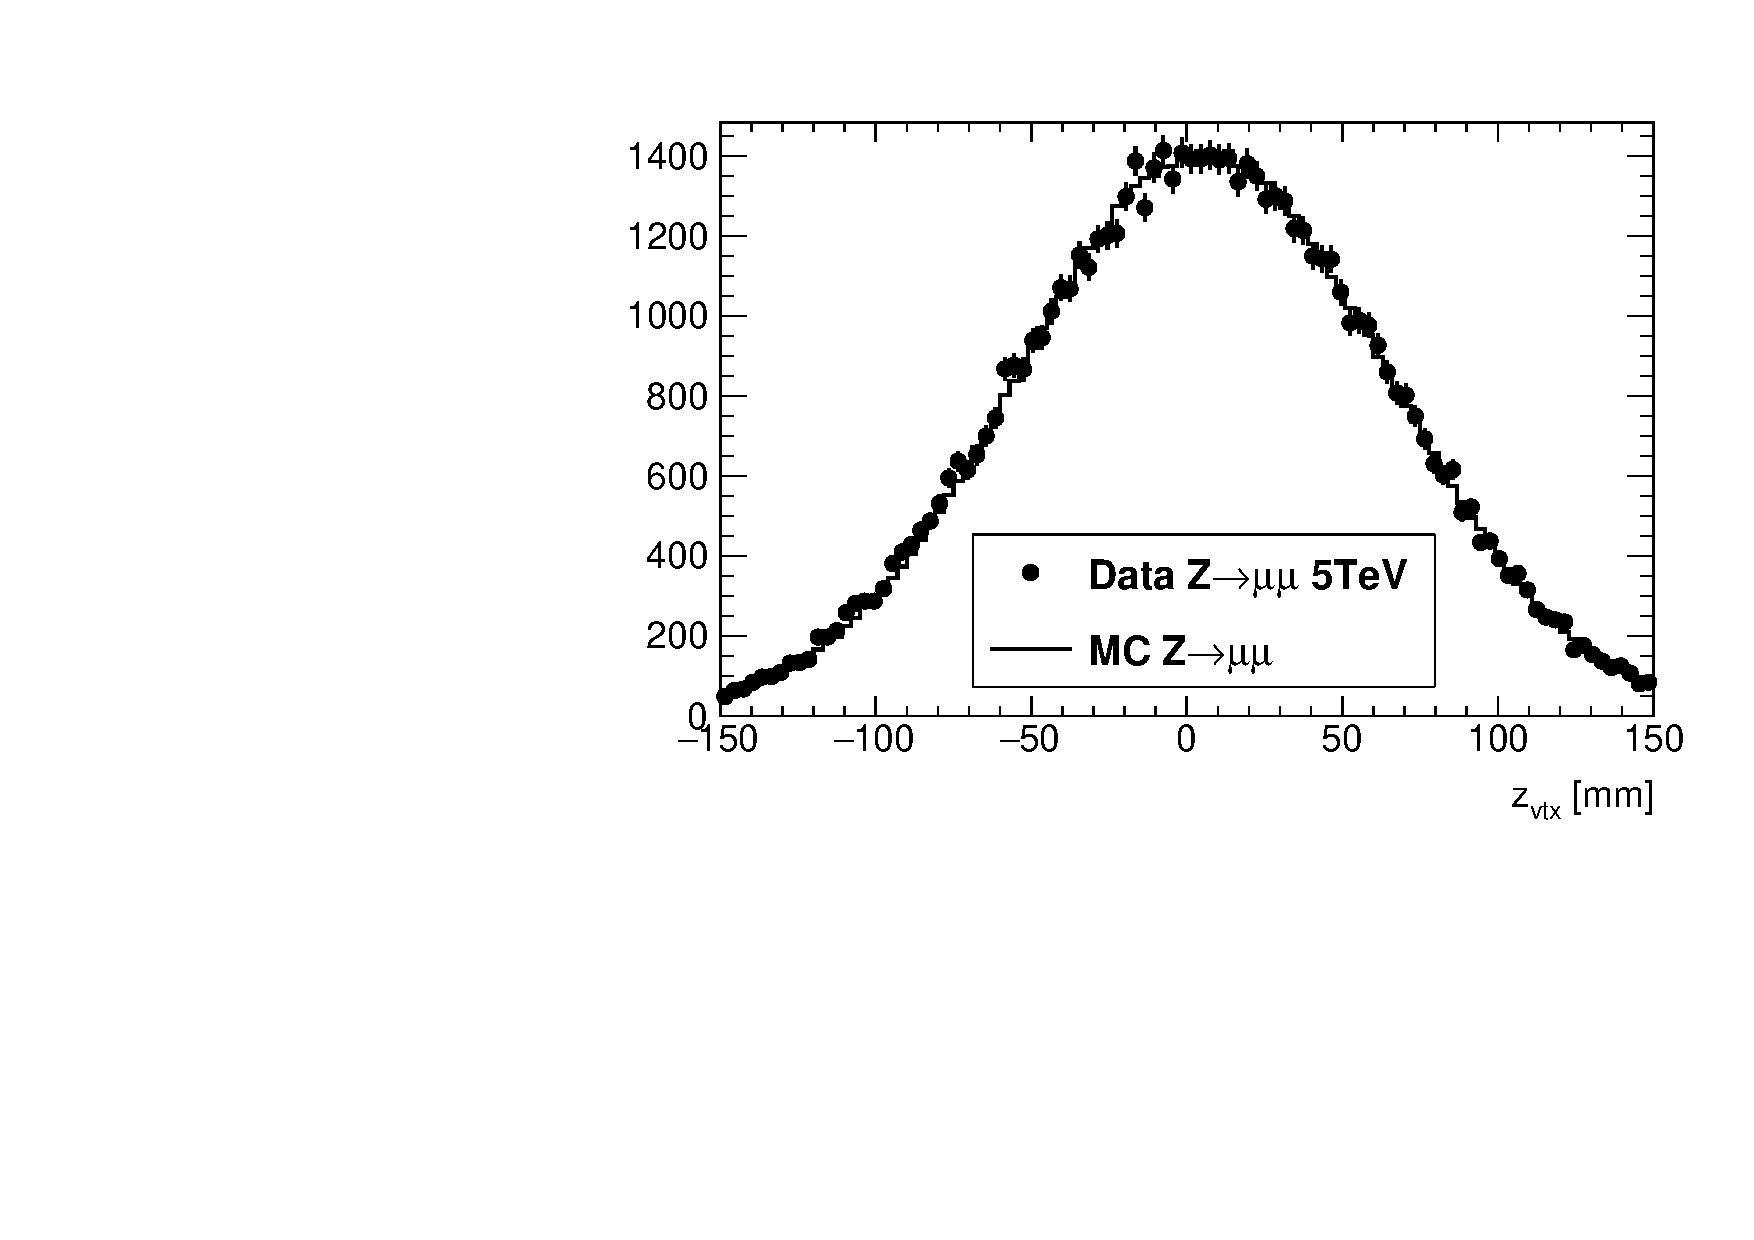
\includegraphics[width=.5\textwidth]{zmumu_5tev_zvtx}%
     	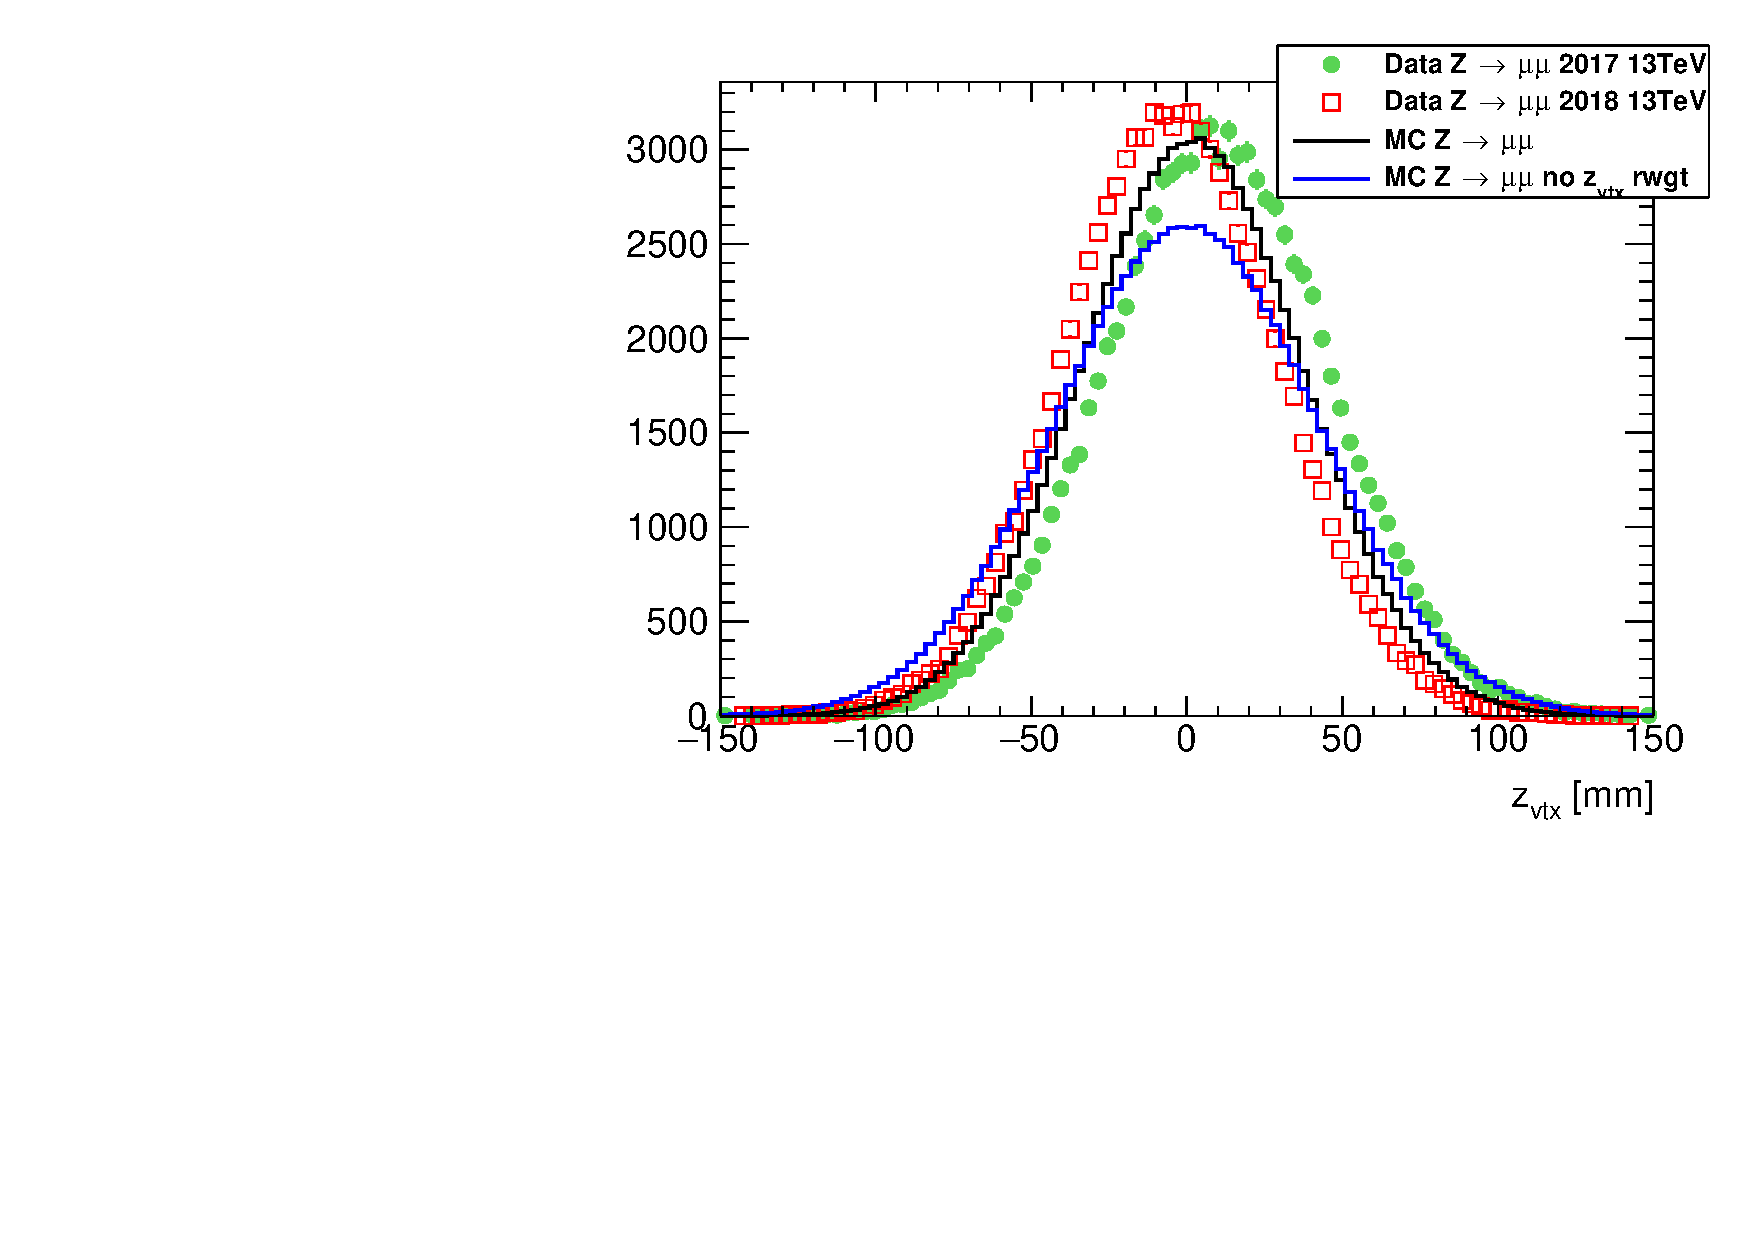
\includegraphics[width=.5\textwidth]{zmumu_13tev_zvtx_norwgt}
     	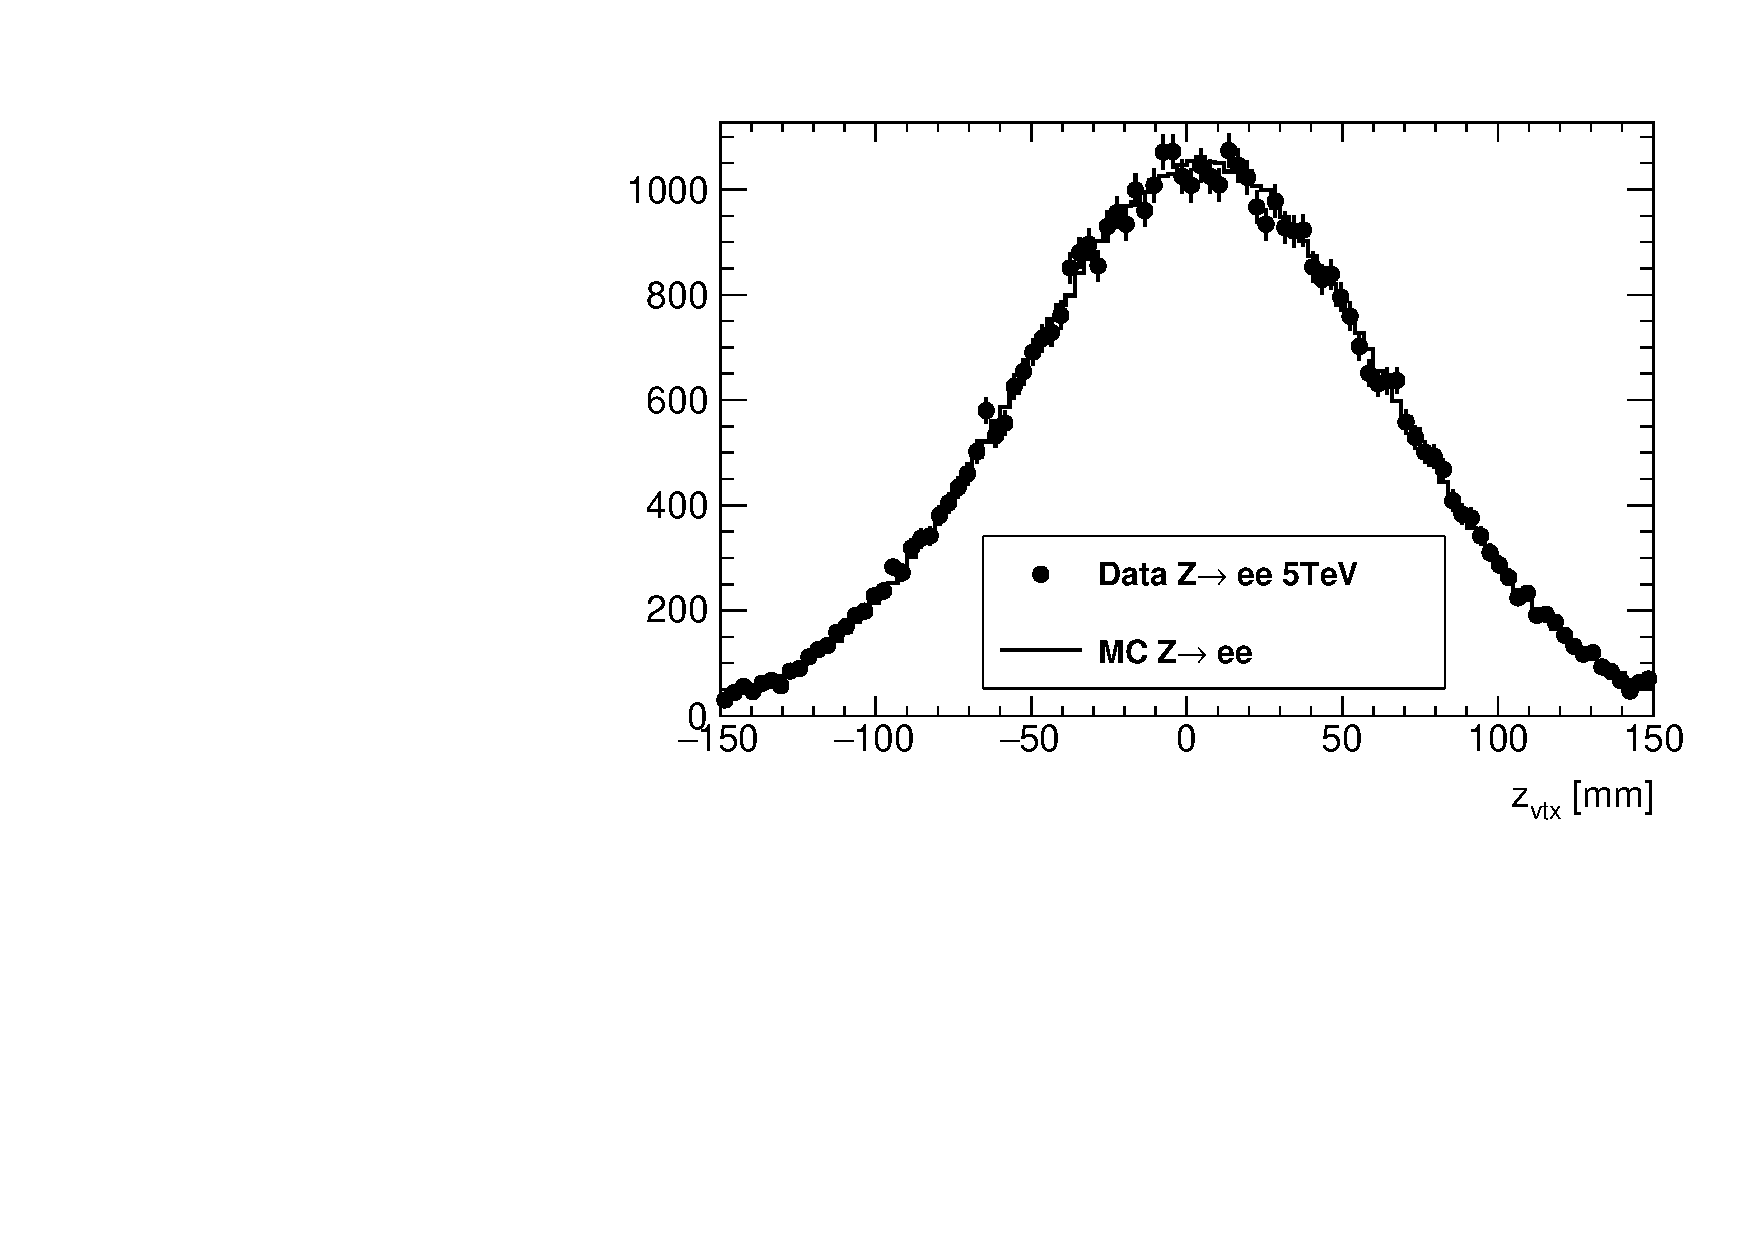
\includegraphics[width=.5\textwidth]{zee_5tev_zvtx}%
     	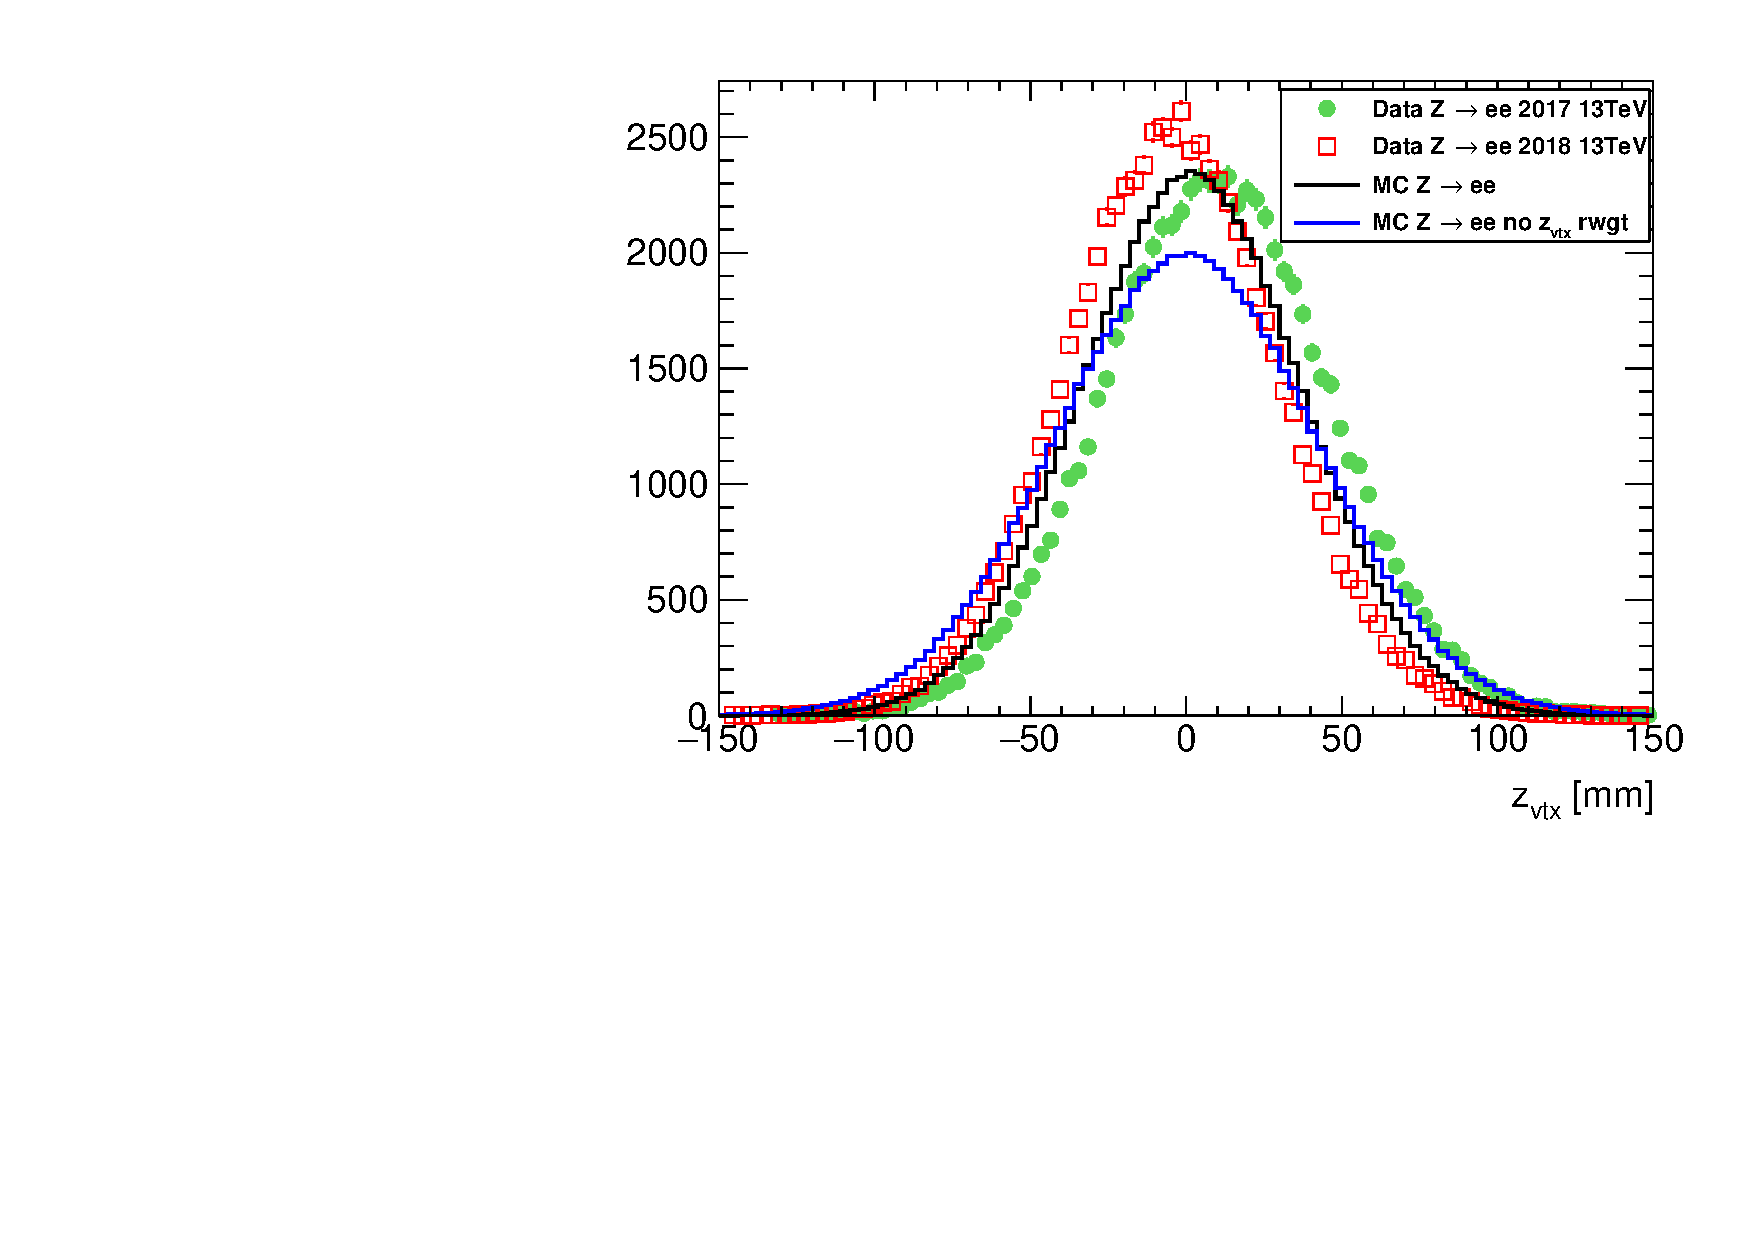
\includegraphics[width=.5\textwidth]{zee_13tev_zvtx_norwgt}
     	\caption{Distributions for the 5 \TeV{} (left) and 13 \TeV{} (right)
     		low-$\mu$ dataset(s) in a \Zgmm (top row) and a \Zgee (bottom row)
     		selection. The data (points) is compared to \Zgmm or \Zgee signal
     		MC, respectively. The distributions of the $z$-position of the
     		primary vertex selected as the hard interaction are compared for
     		the dataset(s) and the MC simulation before (``no $z_\mathrm{vtx}$
     		rwgt'', blue, only 13 \TeV{}) and after reweighting (black). For
     		the 13 \TeV{} data the 2017 and 2018 data are shown separately and
     		all distributions are (roughly) normalised to the same number of
     		selected events in the 2017 dataset. }
     	\label{fig:zvtx}
     \end{figure}
    \subsection{Multijet background}
 The estimate of the multijet background, which contain contributions from fake leptons produced in semi-leptonic decays of heavy quarks, in-flight pion decays, photon conversions, etc, is done using a data-driven techniques described in Reference~\cite{Xu:2657146}. TO BE ADDED.
 
 
\section{W analysis event selection and control plots}
\label{sec:selection}

\subsection{Event selection}
\label{subsec:wselection}
Both in case of 5 and 13~\TeV\ events with \Wln{} candidate were selected base on a single-lepton trigger requirement.
The trigger for \Wen event candidate $\texttt{HLT\_e15\_lhloose\_nod0\_L1EM12}$ require at least one reconstructed electron with \ET larger than 15~\GeV\ passing \emph{loose} identification requirements. Candidates for \Wmn were triggered by $\texttt{HLT\_mu14}$ trigger requiring one muon with \ET larger than 14~\GeV.

Events are required to contain exactly one lepton (muon or electron) candidate having $p_T > 25\gev$. Electrons are required to have $|\eta|<2.47$ excluding transition region $1.37 < |\eta|< 1.52$. Muons   
Events with additional leptons of the same flavour with transverse momentum greater than 20 ~\GeV{} satisfying some ID criteria are discarded, to better reject the \Zboson\ background. The ID point is $medium$ for the muon channel, and $loose$ for the electron channel. There is no requirement on the number of leptons with different flavour than the channel under study.

To suppress background, in particular from multijet processes,
events are required to have \MET{} greater than 25~\GeV{}.
The \Wboson{} boson transverse mass \mt{} is demanded to be larger than 50~\GeV.
This transverse mass is defined as follows:

\begin{equation}\label{eq:mt}
{m}_{T} = \sqrt{2 {p}_{T}^{\nu}p_{T} ^{l} (1-\cos\Delta\phi^{\nu})}
\end{equation}

The tables~\ref{tab:wpen5},\ref{tab:wpmn5},\ref{tab:wmen5},\ref{tab:wmmn5} contain signal selection event yields for the $W^{\pm} \rightarrow \ell^{\pm}\nu$  at $\sqrt{s} = 5~\TeV$ \lowmu dataset. Similarly the tables~\ref{tab:wpen},\ref{tab:wpmn},\ref{tab:wmen},\ref{tab:wmmn} contain the corresponding numbers for the 13~\TeV\ \lowmu\ dataset. Table~\ref{tab:wyields} provides a comparison between observed and expected yields.
Events denoted as \Wln{} in the tables and the plots contain the sum of background events coming from \Wtaunu\ and other \Wboson{} leptonic decays other than the signal.


\begin{table}[h] 
\resizebox{\textwidth}{!}{% 
\begin{tabular}{c|ccc|ccc|ccc|ccc|ccc|ccc|ccc} \toprule
\multicolumn{1}{c}{Cut} &  \multicolumn{3}{c}{Data}  &  \multicolumn{3}{c}{Signal}  &  \multicolumn{3}{c}{$W^{\pm} \rightarrow \ell^{\pm}\nu$ BG}  &  \multicolumn{3}{c}{$Z \rightarrow \ell\ell$}  &  \multicolumn{3}{c}{Top}  &  \multicolumn{3}{c}{Diboson}  &  \multicolumn{3}{c}{Multijet}  \\  \midrule 
One electron & & 1993720 &  & 643610 & $ \pm $ & 260 & 32940 & $ \pm $ & 190 & 44338 & $ \pm $ & 71 & 1754.4 & $ \pm $ & 3.9 & 772.2 & $ \pm $ & 3.7 & & - &  \\
Electron trig matched & & 1907724 &  & 612940 & $ \pm $ & 250 & 30790 & $ \pm $ & 190 & 42100 & $ \pm $ & 69 & 1698.5 & $ \pm $ & 3.8 & 741.1 & $ \pm $ & 3.6 & & - &  \\
Isolation & & 1438941 &  & 610320 & $ \pm $ & 250 & 30590 & $ \pm $ & 190 & 41923 & $ \pm $ & 69 & 1663.6 & $ \pm $ & 3.8 & 722.5 & $ \pm $ & 3.6 & & - &  \\
$p_{T}^{e}>25 \mathrm{GeV}$ & & 720284 &  & 482240 & $ \pm $ & 220 & 14790 & $ \pm $ & 130 & 31955 & $ \pm $ & 53 & 1464.5 & $ \pm $ & 3.5 & 592.1 & $ \pm $ & 3.2 & & - &  \\
$E_{T}^{miss}>25 \mathrm{GeV}$ & & 440605 &  & 421510 & $ \pm $ & 210 & 9650 & $ \pm $ & 100 & 1336 & $ \pm $ & 20 & 1223 & $ \pm $ & 3.2 & 420.8 & $ \pm $ & 2.4 & & - &  \\
$m_{T}>50 \mathrm{GeV}$ & & 430620 &  & 417430 & $ \pm $ & 210 & 8800 & $ \pm $ & 96 & 1047 & $ \pm $ & 16 & 944.3 & $ \pm $ & 2.9 & 373.5 & $ \pm $ & 2.2 & 3030 & $ \pm $ & 550 \\
\bottomrule
\end{tabular}}
\caption{Analysis cut flow for $W^+ \rightarrow e^+\nu$ 5 TeV signal selection. Lepton \pt\ is required to be over 18~\GeV{} before the final cut.}
\label{tab:wpen5}
\end{table}

\begin{table}[h] 
\resizebox{\textwidth}{!}{% 
\begin{tabular}{c|ccc|ccc|ccc|ccc|ccc|ccc|ccc} \toprule
\multicolumn{1}{c}{Cut} &  \multicolumn{3}{c}{Data}  &  \multicolumn{3}{c}{Signal}  &  \multicolumn{3}{c}{$W^{\pm} \rightarrow \ell^{\pm}\nu$ BG}  &  \multicolumn{3}{c}{$Z \rightarrow \ell\ell$}  &  \multicolumn{3}{c}{Top}  &  \multicolumn{3}{c}{Diboson}  &  \multicolumn{3}{c}{Multijet}  \\  \midrule 
One electron & & 7915023 &  & 1797340 & $ \pm $ & 390 & 92520 & $ \pm $ & 270 & 147490 & $ \pm $ & 140 & 63207 & $ \pm $ & 89 & 3069 & $ \pm $ & 63 & & - &  \\
Electron trig matched & & 7840239 &  & 1709140 & $ \pm $ & 380 & 86370 & $ \pm $ & 260 & 139760 & $ \pm $ & 140 & 61110 & $ \pm $ & 88 & 2967 & $ \pm $ & 62 & & - &  \\
Isolation & & 5413483 &  & 1698430 & $ \pm $ & 380 & 85560 & $ \pm $ & 260 & 138890 & $ \pm $ & 140 & 59834 & $ \pm $ & 87 & 2939 & $ \pm $ & 61 & & - &  \\
$p_{T}^{e}>25 \mathrm{GeV}$ & & 2452868 &  & 1342200 & $ \pm $ & 330 & 44450 & $ \pm $ & 190 & 106270 & $ \pm $ & 110 & 53811 & $ \pm $ & 82 & 2565 & $ \pm $ & 58 & & - &  \\
$E_{T}^{miss}>25 \mathrm{GeV}$ & & 1275513 &  & 1136520 & $ \pm $ & 310 & 28580 & $ \pm $ & 150 & 8313 & $ \pm $ & 46 & 45707 & $ \pm $ & 75 & 1990 & $ \pm $ & 53 & & - &  \\
$m_{T}>50 \mathrm{GeV}$ & & 1207776 &  & 1117560 & $ \pm $ & 310 & 24760 & $ \pm $ & 130 & 6443 & $ \pm $ & 36 & 34580 & $ \pm $ & 65 & 1718 & $ \pm $ & 50 & 28000 & $ \pm $ & 1800 \\
\bottomrule
\end{tabular}}
\caption{Analysis cut flow for $W^+ \rightarrow e^+\nu$ 13 TeV signal selection. Lepton \pt\ is required to be over 18~\GeV{} before the final cut.}
\label{tab:wpen}
\end{table}

\begin{table}[h] 
\resizebox{\textwidth}{!}{% 
\begin{tabular}{c|ccc|ccc|ccc|ccc|ccc|ccc|ccc} \toprule
\multicolumn{1}{c}{Cut} &  \multicolumn{3}{c}{Data}  &  \multicolumn{3}{c}{Signal}  &  \multicolumn{3}{c}{$W^{\pm} \rightarrow \ell^{\pm}\nu$ BG}  &  \multicolumn{3}{c}{$Z \rightarrow \ell\ell$}  &  \multicolumn{3}{c}{Top}  &  \multicolumn{3}{c}{Diboson}  &  \multicolumn{3}{c}{Multijet}  \\  \midrule 
One muon & & 2434459 &  & 760980 & $ \pm $ & 280 & 35090 & $ \pm $ & 200 & 37015 & $ \pm $ & 82 & 2025.3 & $ \pm $ & 4.1 & 864.7 & $ \pm $ & 3.7 & & - &  \\
Muon trig matched & & 2353403 &  & 664100 & $ \pm $ & 260 & 30610 & $ \pm $ & 190 & 32554 & $ \pm $ & 76 & 1725.6 & $ \pm $ & 3.8 & 746.6 & $ \pm $ & 3.4 & & - &  \\
Isolation & & 1186616 &  & 659200 & $ \pm $ & 260 & 30400 & $ \pm $ & 190 & 32303 & $ \pm $ & 76 & 1574.6 & $ \pm $ & 3.7 & 710.1 & $ \pm $ & 3.3 & & - &  \\
$p_{T}^{\mu}>25 \mathrm{GeV}$ & & 632016 &  & 508270 & $ \pm $ & 230 & 13900 & $ \pm $ & 130 & 22556 & $ \pm $ & 57 & 1335.3 & $ \pm $ & 3.4 & 568.2 & $ \pm $ & 2.9 & & - &  \\
$E_{T}^{miss}>25 \mathrm{GeV}$ & & 470856 &  & 442600 & $ \pm $ & 210 & 8700 & $ \pm $ & 100 & 9959 & $ \pm $ & 31 & 1111.8 & $ \pm $ & 3 & 424.5 & $ \pm $ & 2.5 & & - &  \\
$m_{T}>50 \mathrm{GeV}$ & & 457053 &  & 438280 & $ \pm $ & 210 & 7879 & $ \pm $ & 97 & 9649 & $ \pm $ & 27 & 879.7 & $ \pm $ & 2.8 & 381.7 & $ \pm $ & 2.3 & 720 & $ \pm $ & 190 \\
\bottomrule
\end{tabular}}
\caption{Analysis cut flow for $W^+ \rightarrow \mu^+\nu$ 5 TeV signal selection. Lepton \pt\ is required to be over 18~\GeV{} before the final cut.}
\label{tab:wpmn5}
\end{table}

\begin{table}[h] 
\resizebox{\textwidth}{!}{% 
\begin{tabular}{c|ccc|ccc|ccc|ccc|ccc|ccc|ccc} \toprule
\multicolumn{1}{c}{Cut} &  \multicolumn{3}{c}{Data}  &  \multicolumn{3}{c}{Signal}  &  \multicolumn{3}{c}{$W^{\pm} \rightarrow \ell^{\pm}\nu$ BG}  &  \multicolumn{3}{c}{$Z \rightarrow \ell\ell$}  &  \multicolumn{3}{c}{Top}  &  \multicolumn{3}{c}{Diboson}  &  \multicolumn{3}{c}{Multijet}  \\  \midrule 
One muon & & 9570104 &  & 2100770 & $ \pm $ & 410 & 83110 & $ \pm $ & 270 & 2019400 & $ \pm $ & 2200 & 71602 & $ \pm $ & 94 & 3442 & $ \pm $ & 63 & & - &  \\
Muon trig matched & & 9382783 &  & 1840550 & $ \pm $ & 390 & 72820 & $ \pm $ & 250 & 1750400 & $ \pm $ & 2000 & 61519 & $ \pm $ & 87 & 2956 & $ \pm $ & 59 & & - &  \\
Isolation & & 3905612 &  & 1821750 & $ \pm $ & 380 & 71780 & $ \pm $ & 250 & 595700 & $ \pm $ & 1100 & 56849 & $ \pm $ & 84 & 2916 & $ \pm $ & 59 & & - &  \\
$p_{T}^{\mu}>25 \mathrm{GeV}$ & & 1930655 &  & 1393330 & $ \pm $ & 340 & 34470 & $ \pm $ & 170 & 170840 & $ \pm $ & 490 & 49338 & $ \pm $ & 78 & 2471 & $ \pm $ & 54 & & - &  \\
$E_{T}^{miss}>25 \mathrm{GeV}$ & & 1321407 &  & 1173860 & $ \pm $ & 310 & 21450 & $ \pm $ & 140 & 51090 & $ \pm $ & 180 & 41956 & $ \pm $ & 72 & 1930 & $ \pm $ & 49 & & - &  \\
$m_{T}>50 \mathrm{GeV}$ & & 1244892 &  & 1153800 & $ \pm $ & 310 & 18270 & $ \pm $ & 130 & 38304 & $ \pm $ & 81 & 32375 & $ \pm $ & 63 & 1705 & $ \pm $ & 44 & 9040 & $ \pm $ & 800 \\
\bottomrule
\end{tabular}}
\caption{Analysis cut flow for $W^+ \rightarrow \mu^+\nu$ 13 TeV signal selection. Lepton \pt\ is required to be over 18~\GeV{} before the final cut.}
\label{tab:wpmn}
\end{table}

\begin{table}[h] 
\resizebox{\textwidth}{!}{% 
\begin{tabular}{c|ccc|ccc|ccc|ccc|ccc|ccc|ccc} \toprule
\multicolumn{1}{c}{Cut} &  \multicolumn{3}{c}{Data}  &  \multicolumn{3}{c}{Signal}  &  \multicolumn{3}{c}{$W^{\pm} \rightarrow \ell^{\pm}\nu$ BG}  &  \multicolumn{3}{c}{$Z \rightarrow \ell\ell$}  &  \multicolumn{3}{c}{Top}  &  \multicolumn{3}{c}{Diboson}  &  \multicolumn{3}{c}{Multijet}  \\  \midrule 
One electron & & 1724472 &  & 374900 & $ \pm $ & 200 & 24150 & $ \pm $ & 160 & 41995 & $ \pm $ & 70 & 1590.5 & $ \pm $ & 2.9 & 684.8 & $ \pm $ & 4 & & - &  \\
Electron trig matched & & 1645694 &  & 359010 & $ \pm $ & 200 & 22070 & $ \pm $ & 160 & 39854 & $ \pm $ & 68 & 1539.9 & $ \pm $ & 2.9 & 655.7 & $ \pm $ & 3.9 & & - &  \\
Isolation & & 1176976 &  & 357660 & $ \pm $ & 200 & 21920 & $ \pm $ & 160 & 39686 & $ \pm $ & 68 & 1504.6 & $ \pm $ & 2.8 & 640.7 & $ \pm $ & 3.8 & & - &  \\
$p_{T}^{e}>25 \mathrm{GeV}$ & & 529183 &  & 302070 & $ \pm $ & 180 & 11920 & $ \pm $ & 110 & 30214 & $ \pm $ & 52 & 1330.8 & $ \pm $ & 2.6 & 532.9 & $ \pm $ & 3.5 & & - &  \\
$E_{T}^{miss}>25 \mathrm{GeV}$ & & 281957 &  & 266750 & $ \pm $ & 170 & 8084 & $ \pm $ & 90 & 1293 & $ \pm $ & 20 & 1112.5 & $ \pm $ & 2.4 & 380 & $ \pm $ & 3 & & - &  \\
$m_{T}>50 \mathrm{GeV}$ & & 274329 &  & 264540 & $ \pm $ & 170 & 7317 & $ \pm $ & 84 & 994 & $ \pm $ & 16 & 855.2 & $ \pm $ & 2.1 & 338.1 & $ \pm $ & 2.9 & 2400 & $ \pm $ & 500 \\
\bottomrule
\end{tabular}}
\caption{Analysis cut flow for $W^- \rightarrow e^-\nu$ 5 TeV signal selection. Lepton \pt\ is required to be over 18~\GeV{} before the final cut.}
\label{tab:wmen5}
\end{table}

\begin{table}[h] 
\resizebox{\textwidth}{!}{% 
\begin{tabular}{c|ccc|ccc|ccc|ccc|ccc|ccc|ccc} \toprule
\multicolumn{1}{c}{Cut} &  \multicolumn{3}{c}{Data}  &  \multicolumn{3}{c}{Signal}  &  \multicolumn{3}{c}{$W^{\pm} \rightarrow \ell^{\pm}\nu$ BG}  &  \multicolumn{3}{c}{$Z \rightarrow \ell\ell$}  &  \multicolumn{3}{c}{Top}  &  \multicolumn{3}{c}{Diboson}  &  \multicolumn{3}{c}{Multijet}  \\  \midrule 
One electron & & 7471742 &  & 1323710 & $ \pm $ & 330 & 78230 & $ \pm $ & 230 & 140980 & $ \pm $ & 140 & 61951 & $ \pm $ & 86 & 3059 & $ \pm $ & 58 & & - &  \\
Electron trig matched & & 7402574 &  & 1267710 & $ \pm $ & 330 & 72240 & $ \pm $ & 230 & 133580 & $ \pm $ & 140 & 59950 & $ \pm $ & 85 & 2968 & $ \pm $ & 57 & & - &  \\
Isolation & & 4949352 &  & 1260540 & $ \pm $ & 330 & 71550 & $ \pm $ & 230 & 132740 & $ \pm $ & 140 & 58689 & $ \pm $ & 84 & 2937 & $ \pm $ & 57 & & - &  \\
$p_{T}^{e}>25 \mathrm{GeV}$ & & 2113364 &  & 1053510 & $ \pm $ & 300 & 39660 & $ \pm $ & 160 & 101350 & $ \pm $ & 110 & 52923 & $ \pm $ & 79 & 2544 & $ \pm $ & 53 & & - &  \\
$E_{T}^{miss}>25 \mathrm{GeV}$ & & 1008915 &  & 900640 & $ \pm $ & 280 & 25900 & $ \pm $ & 130 & 7954 & $ \pm $ & 45 & 45065 & $ \pm $ & 73 & 1962 & $ \pm $ & 48 & & - &  \\
$m_{T}>50 \mathrm{GeV}$ & & 949362 &  & 887810 & $ \pm $ & 270 & 22400 & $ \pm $ & 120 & 6052 & $ \pm $ & 35 & 34177 & $ \pm $ & 64 & 1695 & $ \pm $ & 44 & 27400 & $ \pm $ & 2000 \\
\bottomrule
\end{tabular}}
\caption{Analysis cut flow for $W^- \rightarrow e^-\nu$ 13 TeV signal selection. Lepton \pt\ is required to be over 18~\GeV{} before the final cut.}
\label{tab:wmen}
\end{table}

\begin{table}[h] 
\resizebox{\textwidth}{!}{% 
\begin{tabular}{c|ccc|ccc|ccc|ccc|ccc|ccc|ccc} \toprule
\multicolumn{1}{c}{Cut} &  \multicolumn{3}{c}{Data}  &  \multicolumn{3}{c}{Signal}  &  \multicolumn{3}{c}{$W^{\pm} \rightarrow \ell^{\pm}\nu$ BG}  &  \multicolumn{3}{c}{$Z \rightarrow \ell\ell$}  &  \multicolumn{3}{c}{Top}  &  \multicolumn{3}{c}{Diboson}  &  \multicolumn{3}{c}{Multijet}  \\  \midrule 
One muon & & 2075709 &  & 440560 & $ \pm $ & 220 & 22510 & $ \pm $ & 170 & 34440 & $ \pm $ & 80 & 1835.6 & $ \pm $ & 3.1 & 751.5 & $ \pm $ & 3.3 & & - &  \\
Muon trig matched & & 2002955 &  & 383720 & $ \pm $ & 200 & 19640 & $ \pm $ & 160 & 30277 & $ \pm $ & 75 & 1561.6 & $ \pm $ & 2.9 & 648 & $ \pm $ & 3.1 & & - &  \\
Isolation & & 883078 &  & 381010 & $ \pm $ & 200 & 19450 & $ \pm $ & 160 & 30046 & $ \pm $ & 74 & 1411 & $ \pm $ & 2.7 & 616.9 & $ \pm $ & 2.9 & & - &  \\
$p_{T}^{\mu}>25 \mathrm{GeV}$ & & 426119 &  & 314370 & $ \pm $ & 180 & 9370 & $ \pm $ & 110 & 20749 & $ \pm $ & 56 & 1202.1 & $ \pm $ & 2.5 & 505 & $ \pm $ & 2.5 & & - &  \\
$E_{T}^{miss}>25 \mathrm{GeV}$ & & 298992 &  & 276060 & $ \pm $ & 170 & 5893 & $ \pm $ & 89 & 8716 & $ \pm $ & 29 & 1004.2 & $ \pm $ & 2.3 & 372.6 & $ \pm $ & 2 & & - &  \\
$m_{T}>50 \mathrm{GeV}$ & & 287870 &  & 273710 & $ \pm $ & 170 & 5158 & $ \pm $ & 82 & 8408 & $ \pm $ & 26 & 788.2 & $ \pm $ & 2 & 335.6 & $ \pm $ & 1.9 & 760 & $ \pm $ & 160 \\
\bottomrule
\end{tabular}}
\caption{Analysis cut flow for $W^- \rightarrow \mu^-\nu$ 5 TeV signal selection. Lepton \pt\ is required to be over 18~\GeV{} before the final cut.}
\label{tab:wmmn5}
\end{table}

\begin{table}[h] 
\resizebox{\textwidth}{!}{% 
\begin{tabular}{c|ccc|ccc|ccc|ccc|ccc|ccc|ccc} \toprule
\multicolumn{1}{c}{Cut} &  \multicolumn{3}{c}{Data}  &  \multicolumn{3}{c}{Signal}  &  \multicolumn{3}{c}{$W^{\pm} \rightarrow \ell^{\pm}\nu$ BG}  &  \multicolumn{3}{c}{$Z \rightarrow \ell\ell$}  &  \multicolumn{3}{c}{Top}  &  \multicolumn{3}{c}{Diboson}  &  \multicolumn{3}{c}{Multijet}  \\  \midrule 
One muon & & 8773414 &  & 1518070 & $ \pm $ & 360 & 64930 & $ \pm $ & 230 & 2019900 & $ \pm $ & 2200 & 70580 & $ \pm $ & 90 & 3230 & $ \pm $ & 60 & & - &  \\
Muon trig matched & & 8597493 &  & 1322980 & $ \pm $ & 330 & 56520 & $ \pm $ & 210 & 1750300 & $ \pm $ & 2000 & 60579 & $ \pm $ & 84 & 2806 & $ \pm $ & 56 & & - &  \\
Isolation & & 3298569 &  & 1310310 & $ \pm $ & 330 & 55680 & $ \pm $ & 210 & 593700 & $ \pm $ & 1100 & 55949 & $ \pm $ & 80 & 2751 & $ \pm $ & 55 & & - &  \\
$p_{T}^{\mu}>25 \mathrm{GeV}$ & & 1561721 &  & 1069770 & $ \pm $ & 300 & 28230 & $ \pm $ & 150 & 166810 & $ \pm $ & 490 & 48544 & $ \pm $ & 75 & 2362 & $ \pm $ & 52 & & - &  \\
$E_{T}^{miss}>25 \mathrm{GeV}$ & & 1030406 &  & 910150 & $ \pm $ & 280 & 17380 & $ \pm $ & 120 & 47370 & $ \pm $ & 180 & 41259 & $ \pm $ & 69 & 1842 & $ \pm $ & 46 & & - &  \\
$m_{T}>50 \mathrm{GeV}$ & & 963568 &  & 896850 & $ \pm $ & 270 & 14710 & $ \pm $ & 110 & 34572 & $ \pm $ & 80 & 31772 & $ \pm $ & 61 & 1598 & $ \pm $ & 43 & 9050 & $ \pm $ & 620 \\
\bottomrule
\end{tabular}}
\caption{Analysis cut flow for $W^- \rightarrow \mu^-\nu$ 13 TeV signal selection. Lepton \pt\ is required to be over 18~\GeV{} before the final cut.}
\label{tab:wmmn}
\end{table}

\begin{table}[h] 
\centering
\begin{tabular}{c|ccc|ccc} \toprule
\multicolumn{1}{c}{Selection} & \multicolumn{3}{c}{Observed} & \multicolumn{3}{c}{Expected} \\ \midrule
$5\TeV  \;  W^+ \rightarrow e^+\nu$  & & 430620 & & 431620 & $ \pm $ & 600\\
$5\TeV  \;  W^+ \rightarrow \mu^+\nu$ & & 457053 & & 457790 & $ \pm $ & 300\\
$5\TeV  \;  W^- \rightarrow e^-\nu$ & & 274329 & & 276450 & $ \pm $ & 530\\
$5\TeV  \;  W^- \rightarrow \mu^-\nu$ & & 287870 & & 289160 & $ \pm $ & 250\\
$13\TeV  \;  W^+ \rightarrow e^+\nu$  & & 1207776 & & 1213000 & $ \pm $ & 1800\\
$13\TeV  \;  W^+ \rightarrow \mu^+\nu$ & & 1244892 & & 1253490 & $ \pm $ & 870\\
$13\TeV  \;  W^- \rightarrow e^-\nu$ & & 949362 & & 979500 & $ \pm $ & 2000\\
$13\TeV  \;  W^- \rightarrow \mu^-\nu$ & & 963568 & & 988560 & $ \pm $ & 690\\
\bottomrule
\end{tabular}
\caption{Observed and Expected yield comparison for all signal selections.}
\label{tab:wyields}
\end{table}


%\clearpage


\subsection{$\sqrt{s} = 13$~\TeV\ dataset control plots}
\label{subsec:controlplots13}
Control plots for the 13~\TeV\ \lowmu\ dataset are provided here after applying all corrections described in section~\ref{sec:objects}, and after applying the selection described above in this section. In each figure, the right(left)-hand column shows distributions for the \Wplus\ (\Wminus) process. The top (bottom) row shows the muon (electron) decay channel. In the ratio panels, the grey band is the total systematic uncertainty, whilst the brown band adds the MC statistical uncertainty in quadrature on top of it. In regions of the distributions insensitive to the modelling of \ptw\ there is generally good agreement between data and predictions. The bulk of the \mt\ distribution is a typical example of distribution that is mostly insensitive to the modeling of \ptw. The \ut\ distribution is an exception, and it can therefore be concluded that the baseline simulation is not modeling \ptw\ satisfactorily.
\newpage
%%%%%%%%%%%%%%%%%%%%%%%%%%%%%%%%_log.
%%%%% ************************* 13 TeV ****************************
%%%%%%%%%%%%%%%%%%%%%%%%%%%%%%%%


\begin{figure}[h]
	\centering
	{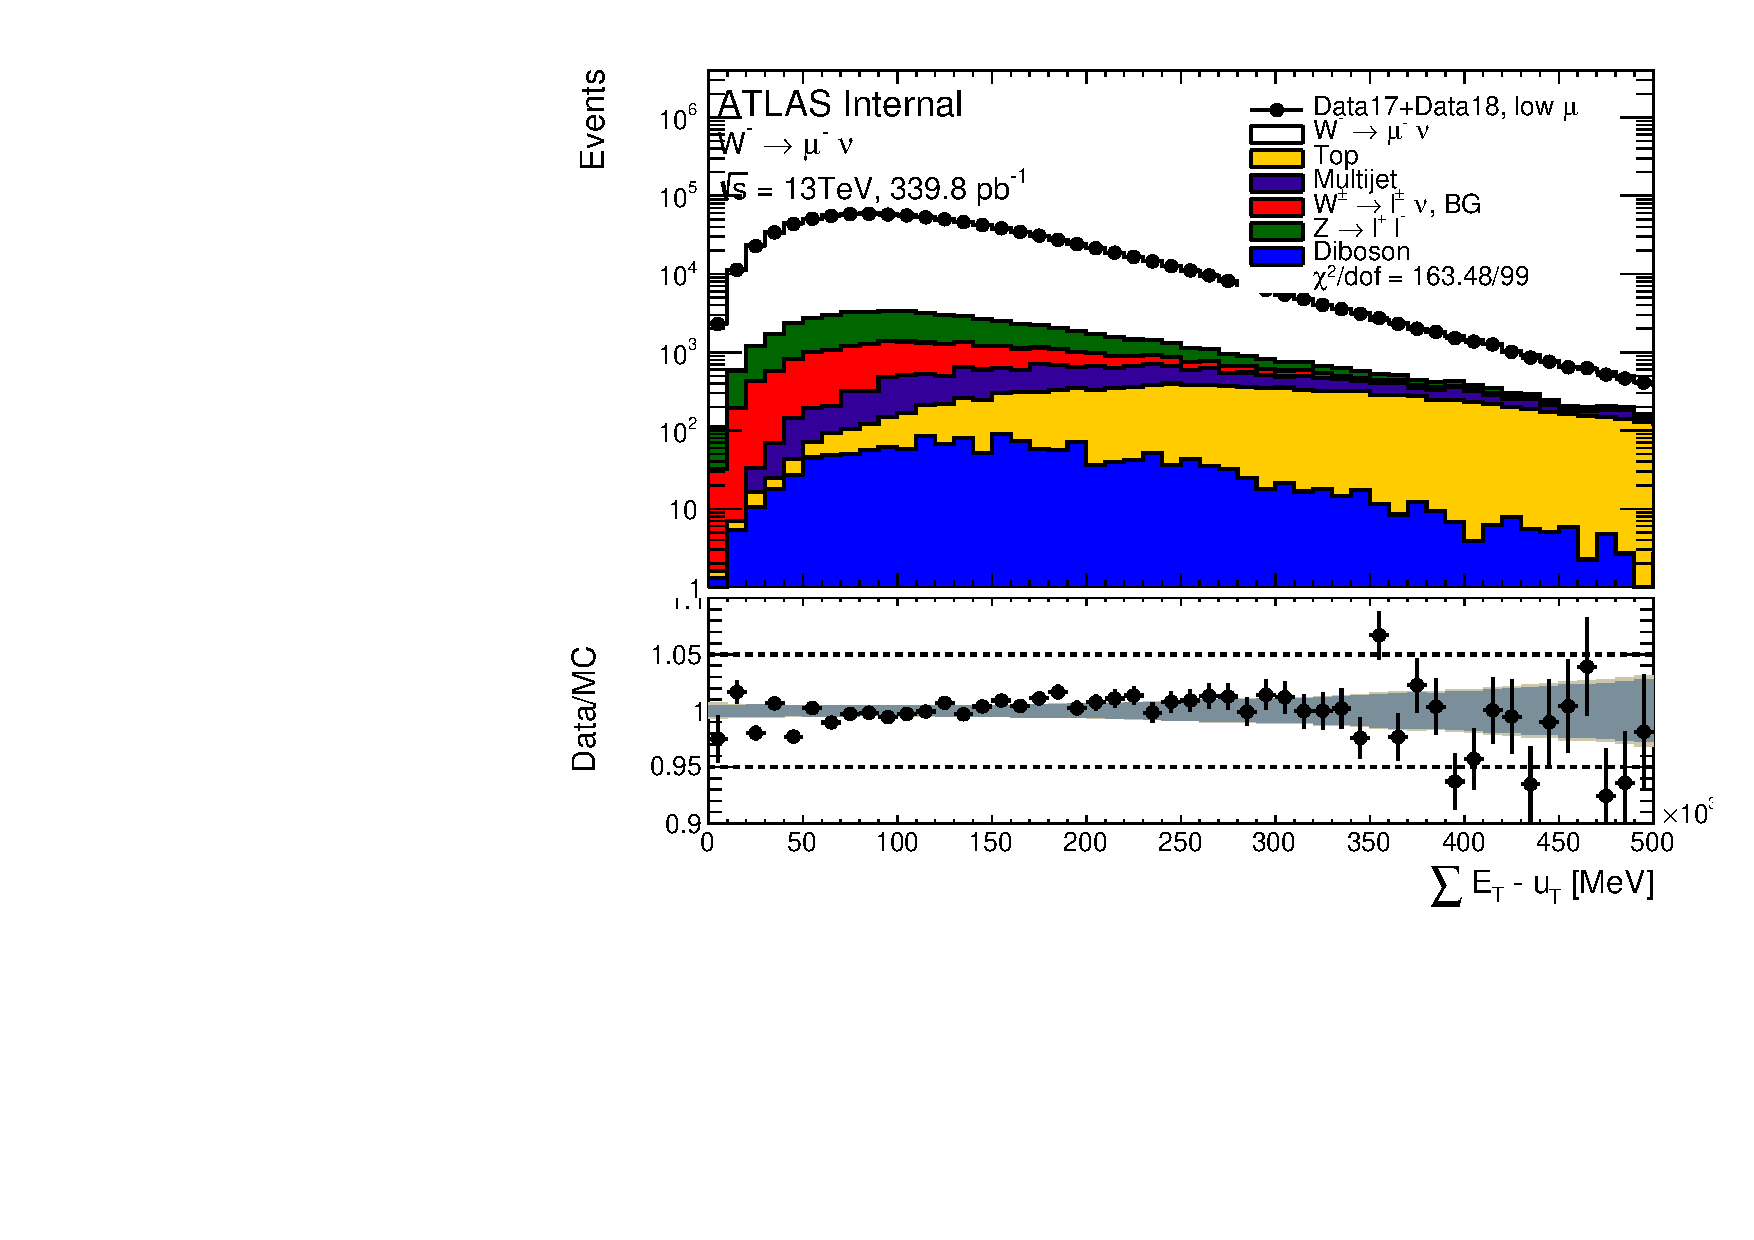
\includegraphics[width=.49\textwidth]{control_norm/SETUE_cut7_minusmunu_13TeV_log_norm_NormErr.pdf}\label{f:SETUEmm13}}
	{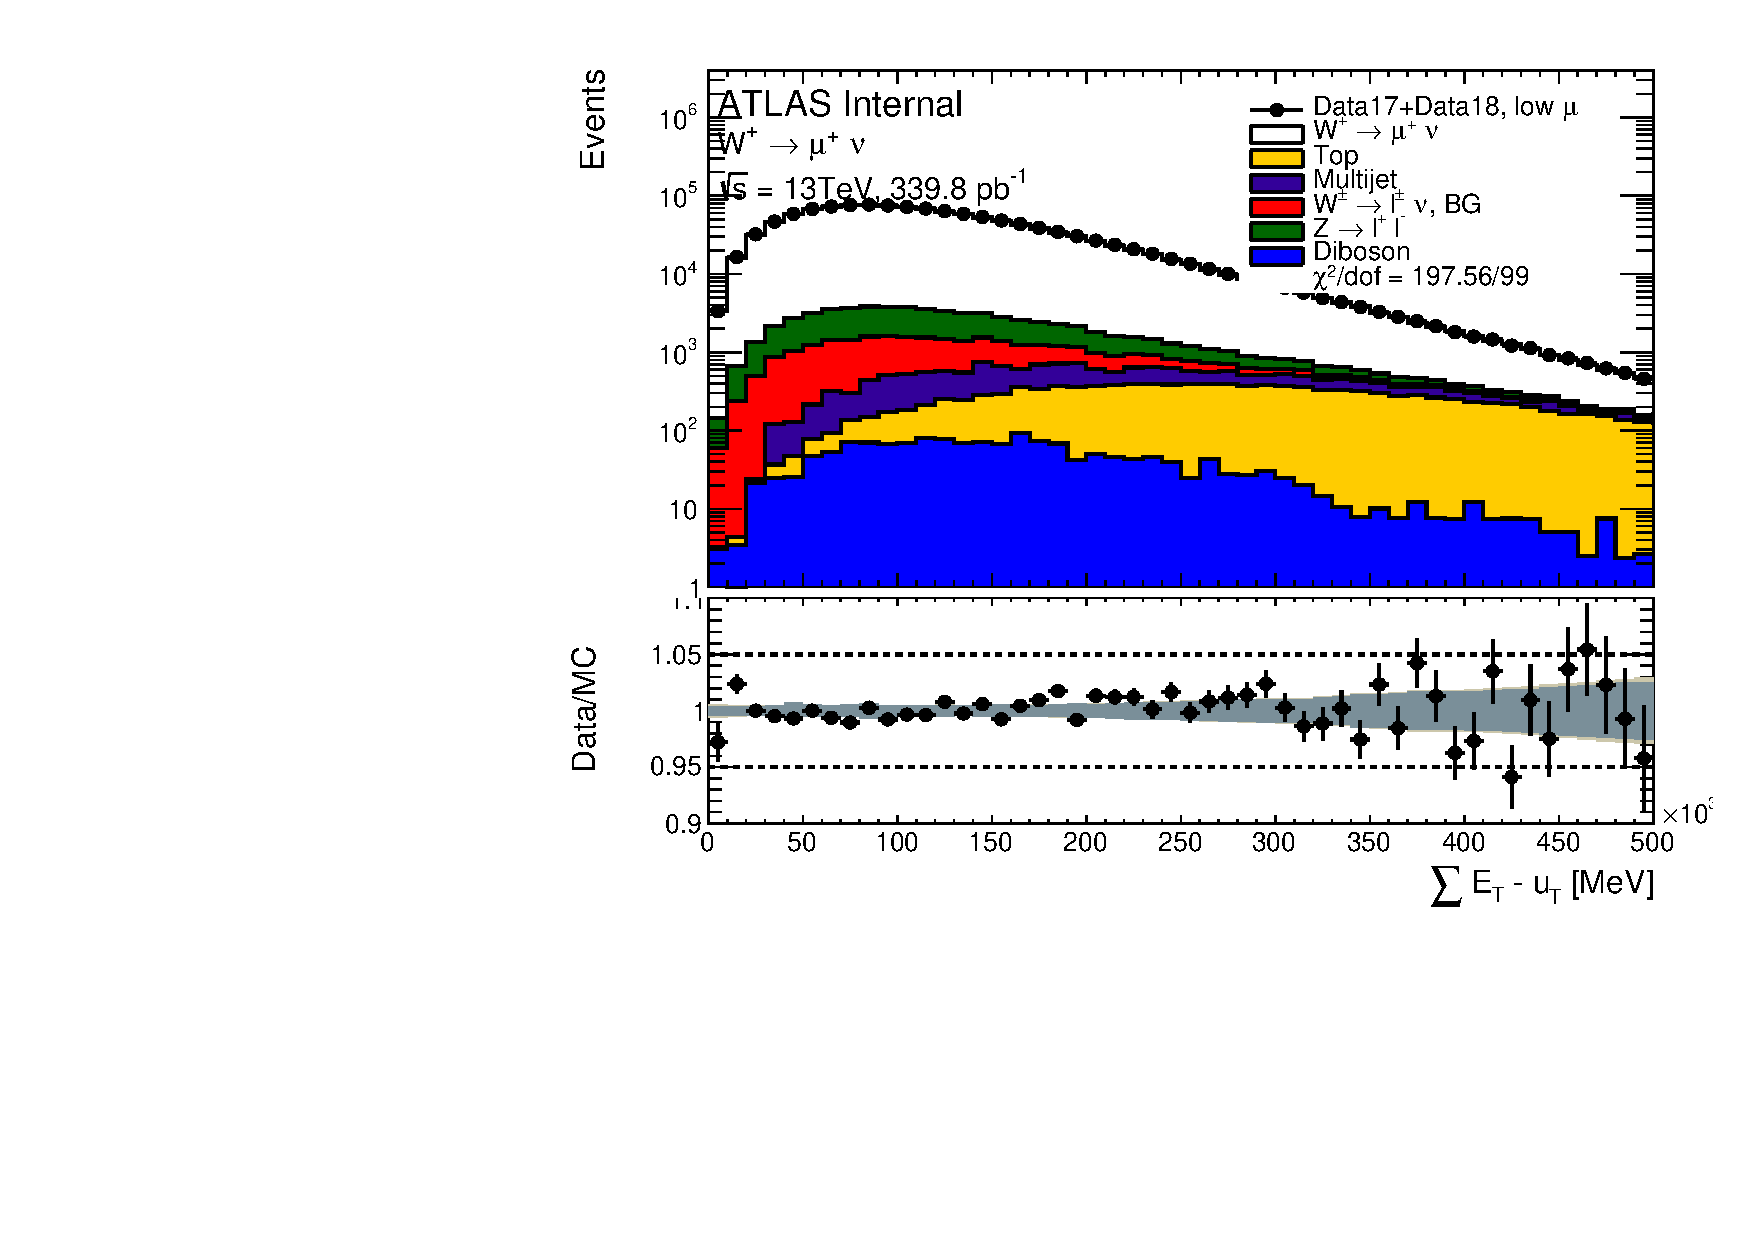
\includegraphics[width=.49\textwidth]{control_norm/SETUE_cut7_plusmunu_13TeV_log_norm_NormErr.pdf}\label{f:SETUEpm13}}
	
	{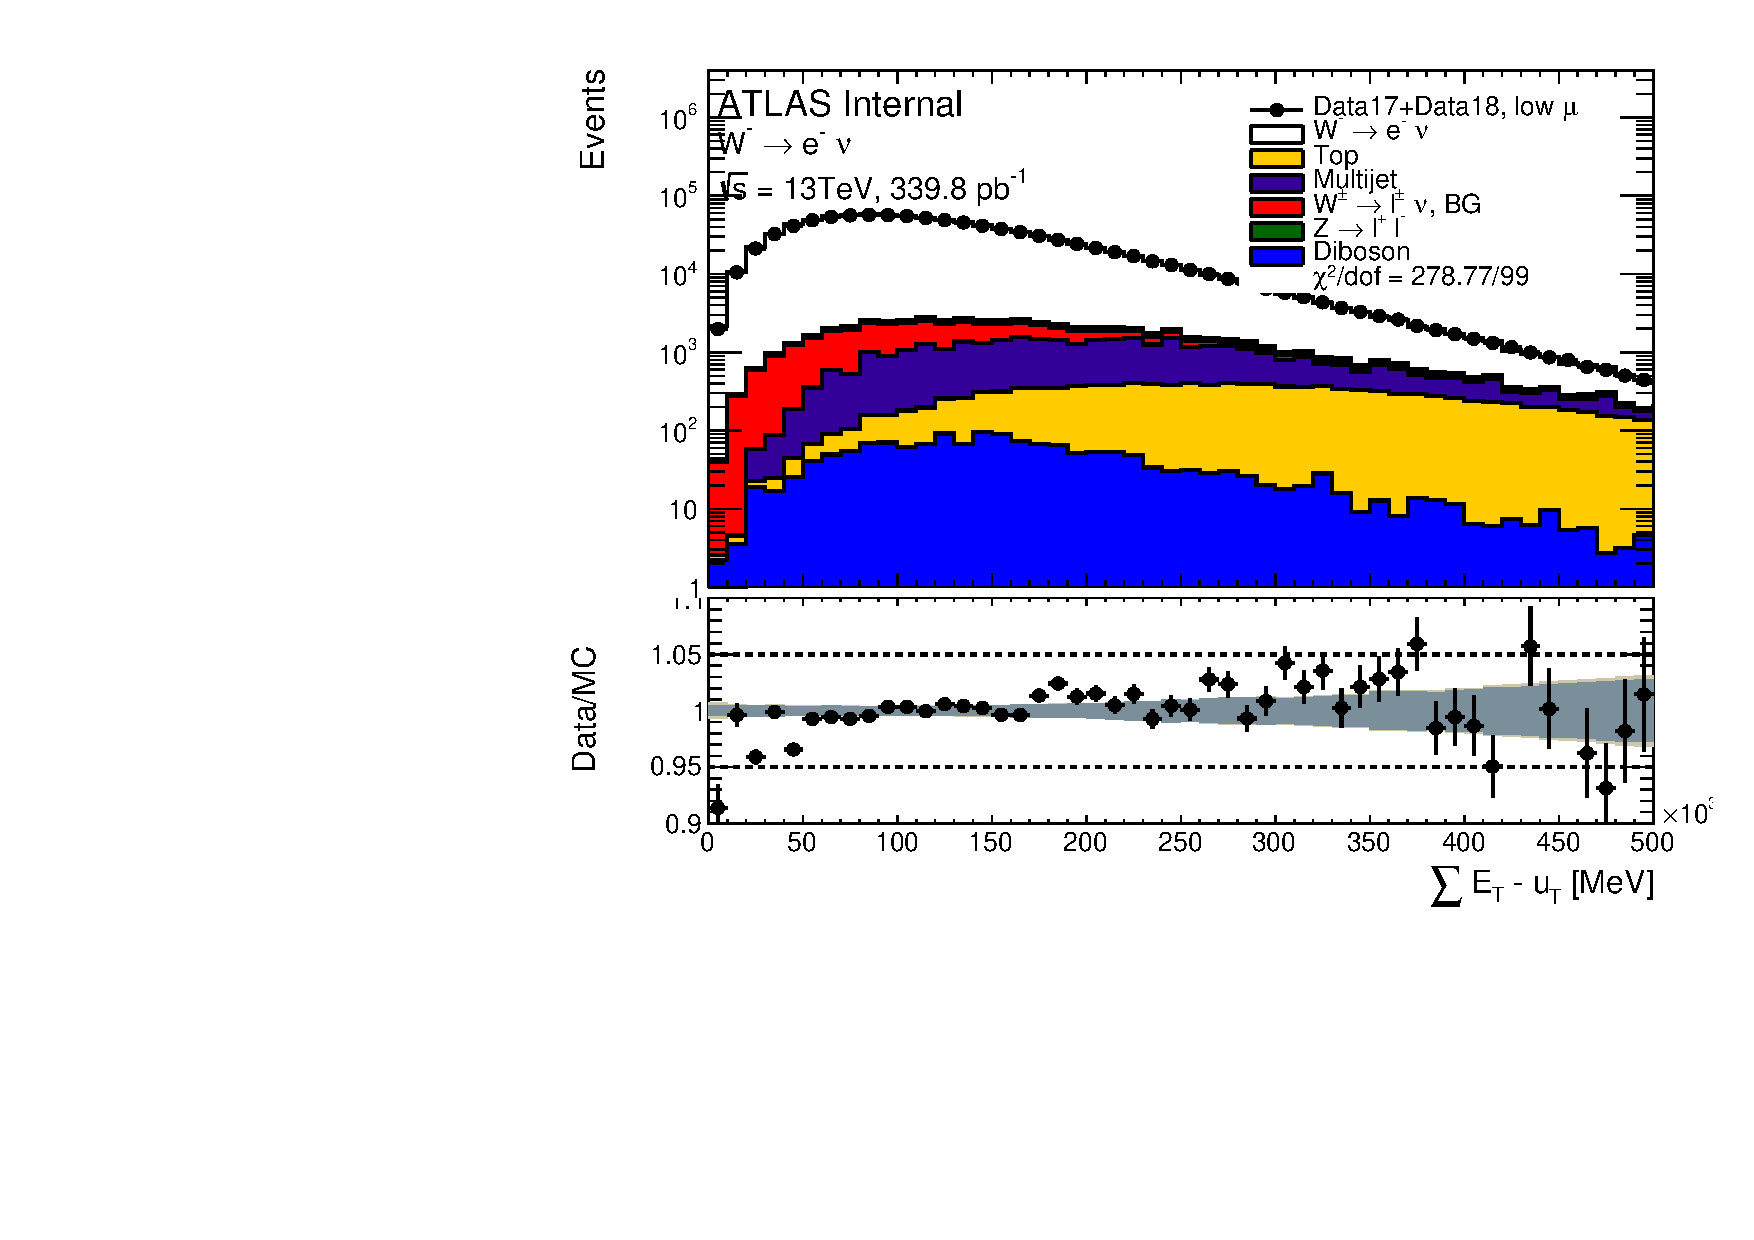
\includegraphics[width=.49\textwidth]{control_norm/SETUE_cut7_minusenu_13TeV_log_norm_NormErr.pdf}\label{f:}}
	{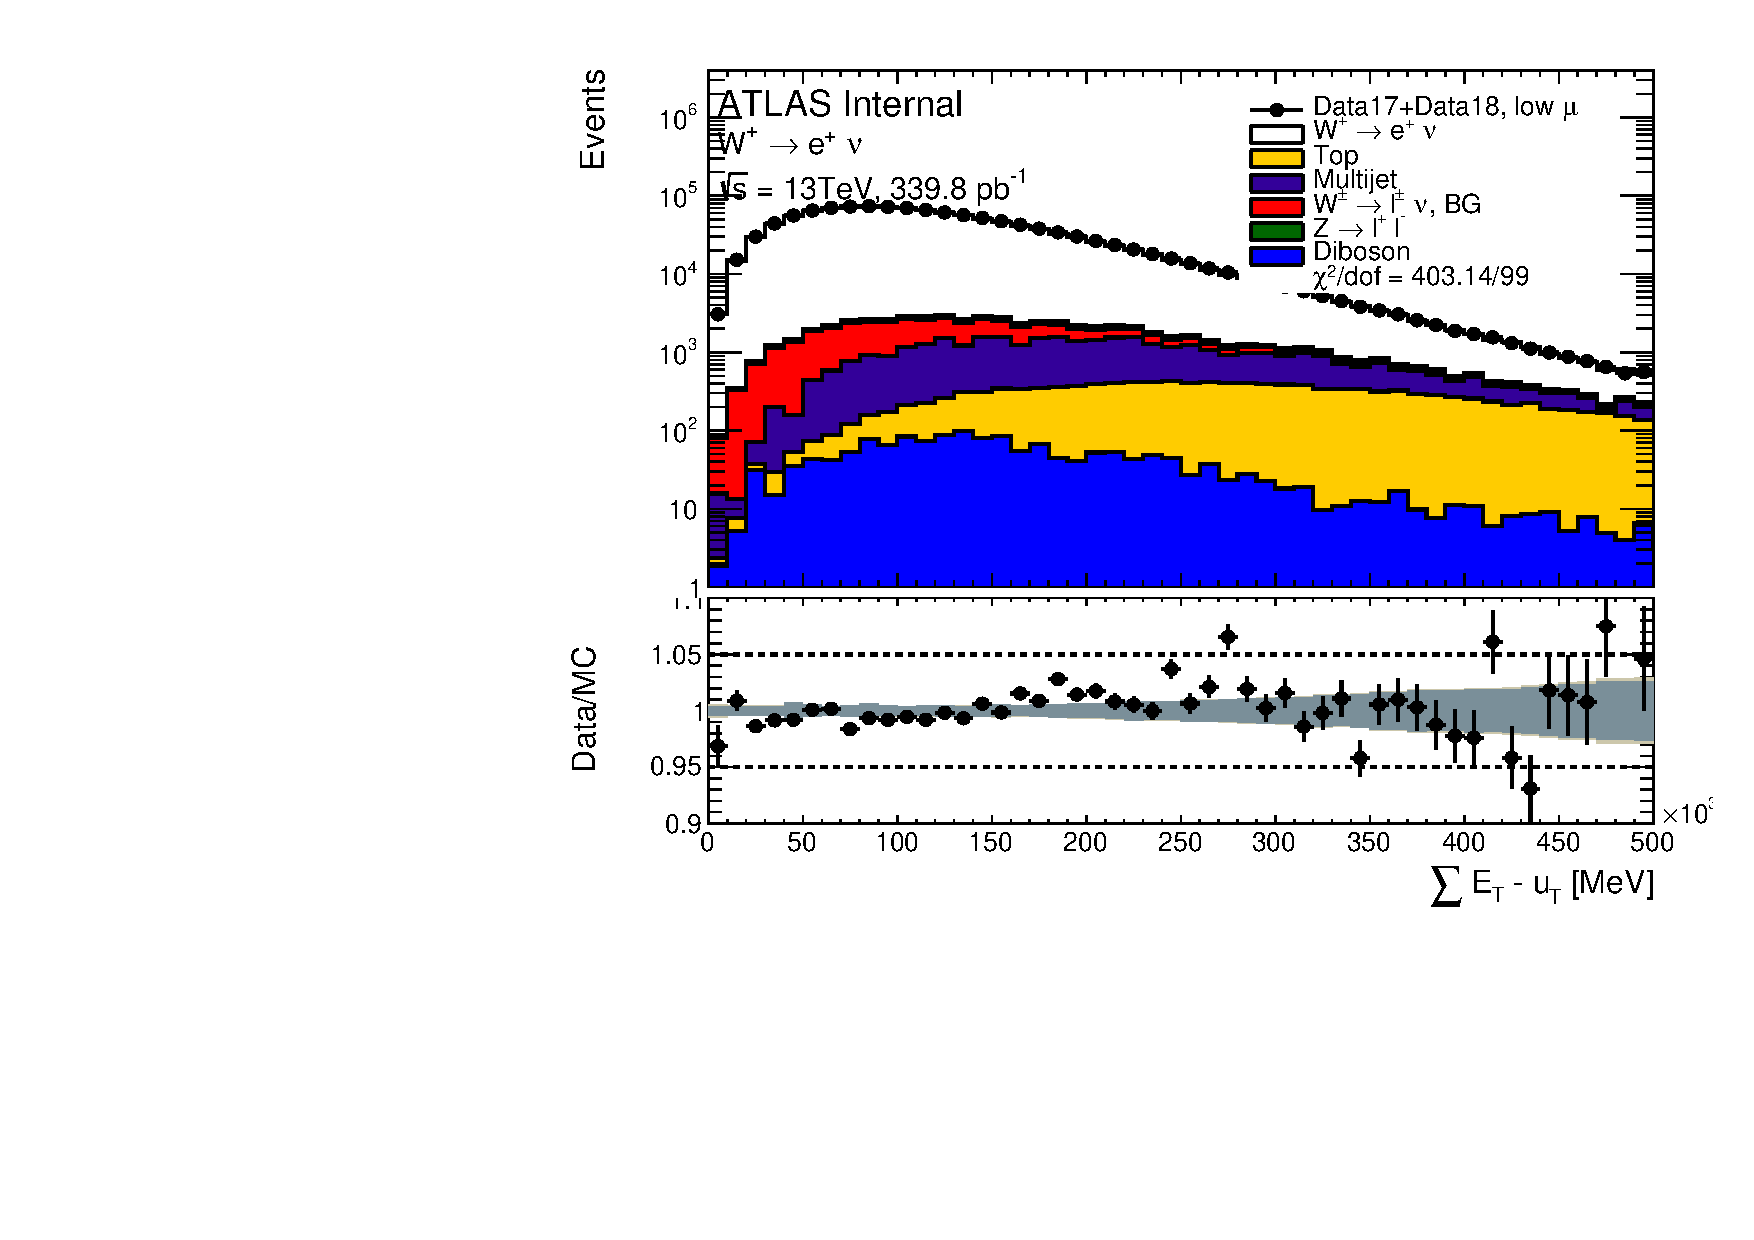
\includegraphics[width=.49\textwidth]{control_norm/SETUE_cut7_plusenu_13TeV_log_norm_NormErr.pdf}\label{f:}}
	\caption{$\Sigma \bar{E_T}$ distribution in the muon and electron channel  for the $\sqrt{s} = 13$~\TeV\ dataset.}\end{figure}
%

\begin{figure}[h]
	\centering
	{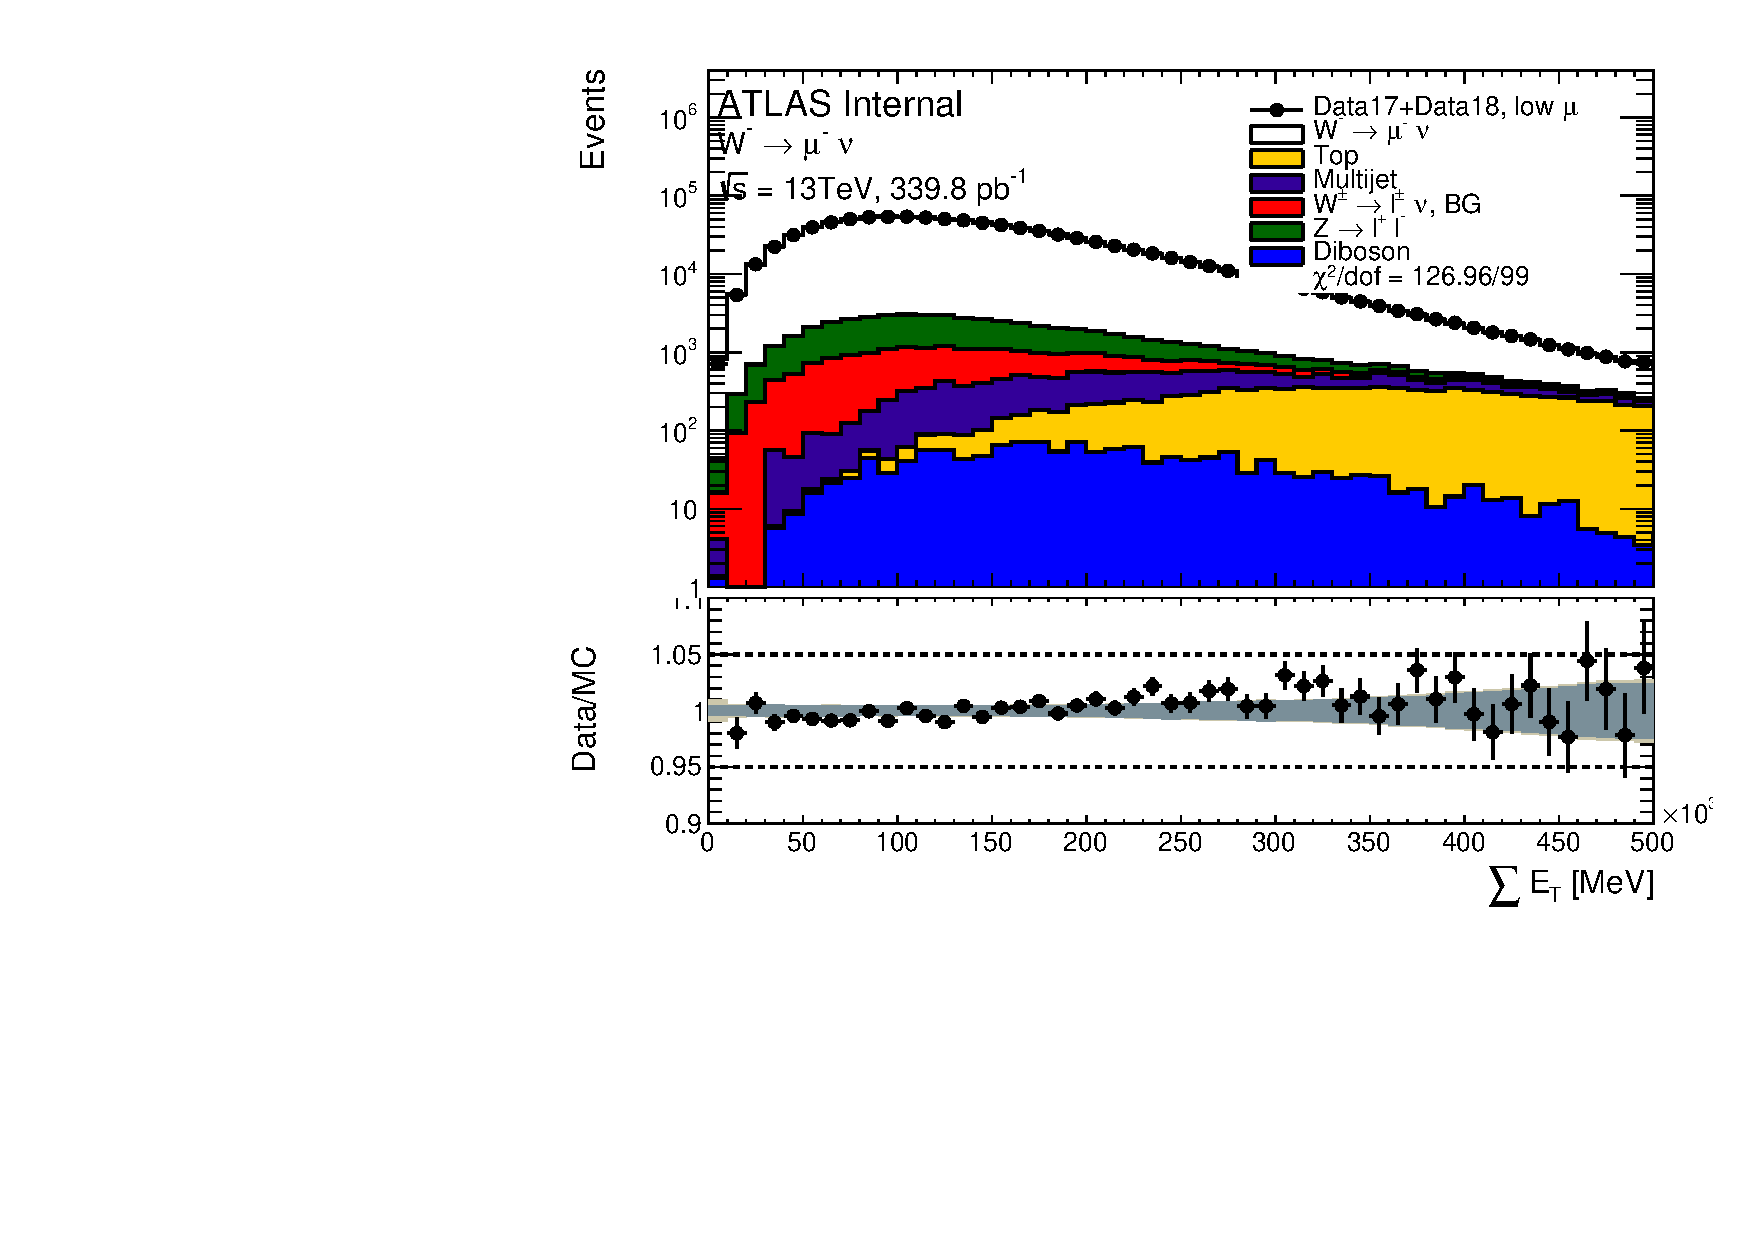
\includegraphics[width=.49\textwidth]{control_norm/SET_cut7_minusmunu_13TeV_log_norm_NormErr.pdf}\label{f:set13}}
	{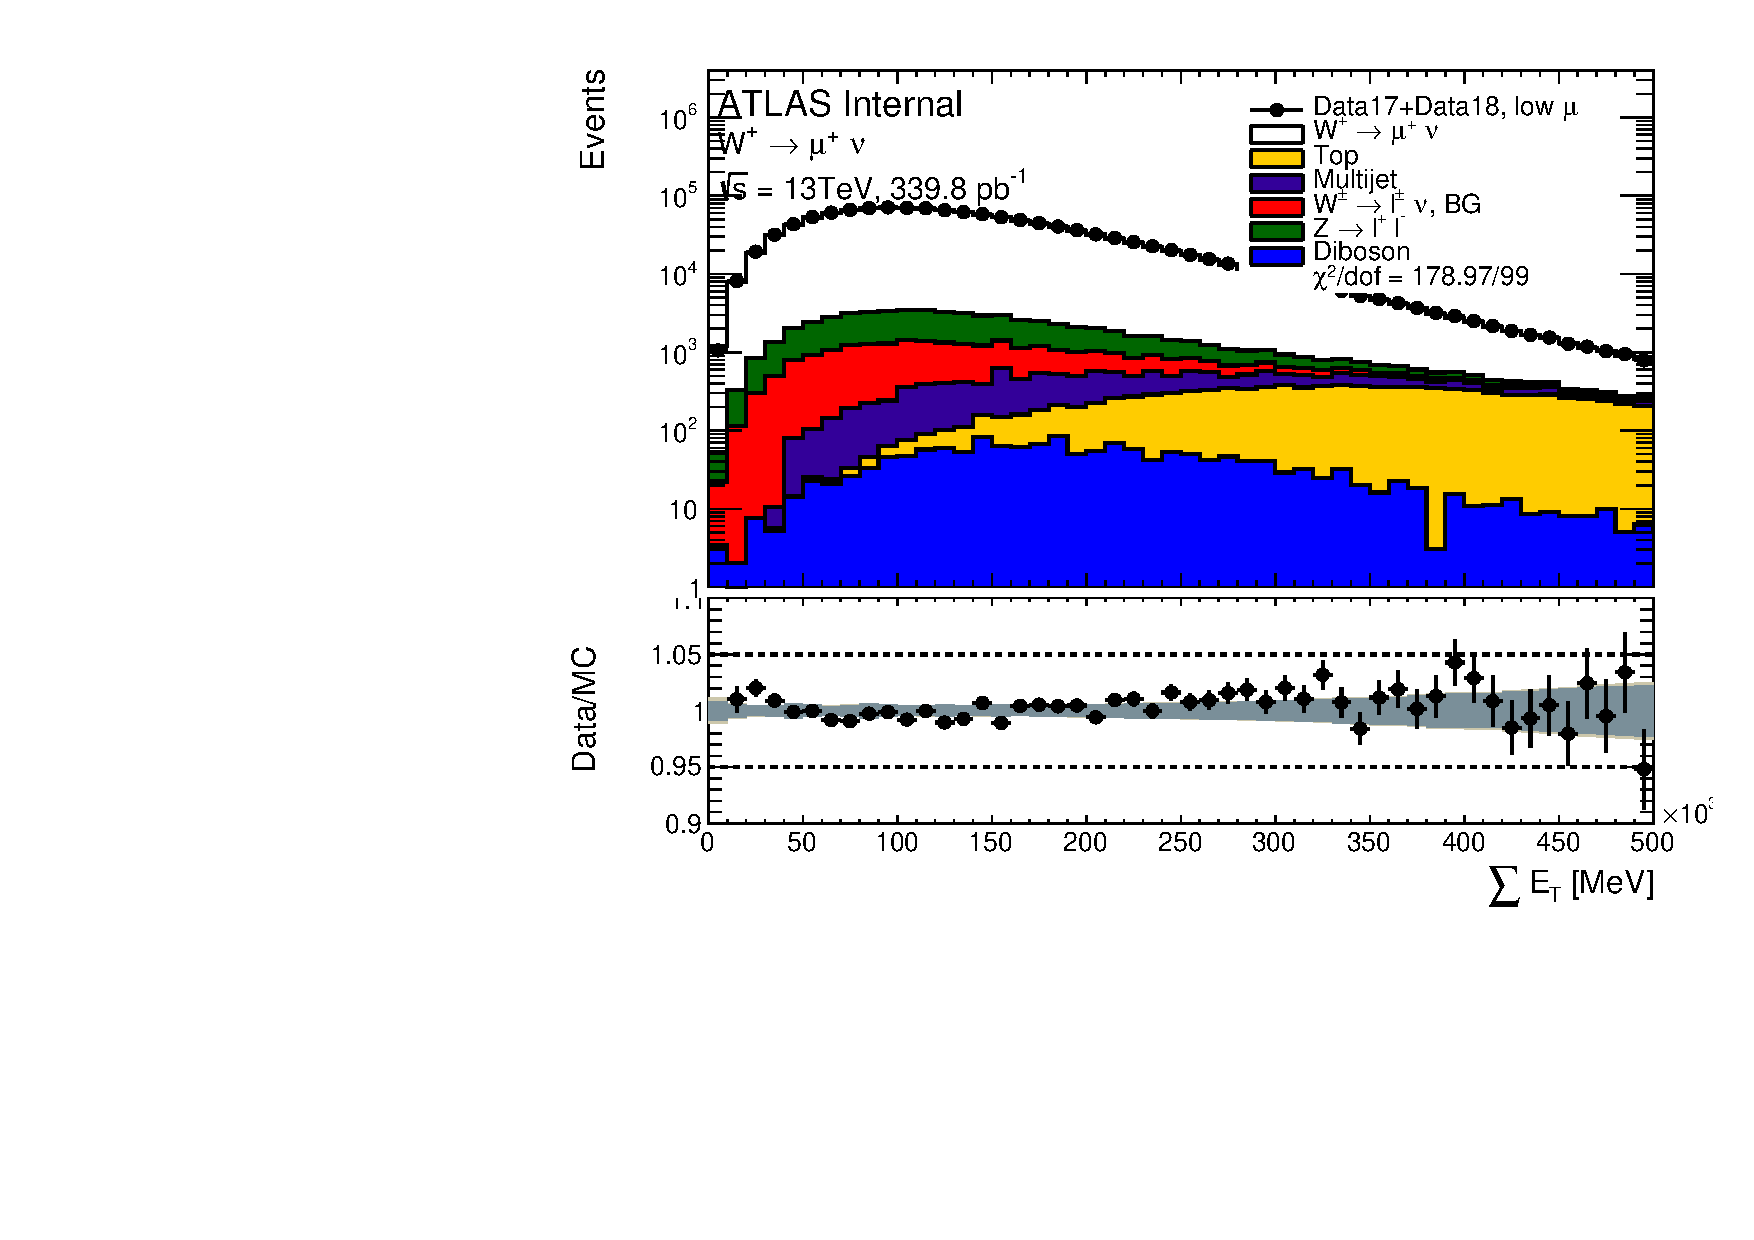
\includegraphics[width=.49\textwidth]{control_norm/SET_cut7_plusmunu_13TeV_log_norm_NormErr.pdf}\label{f:setpl}}
	
	{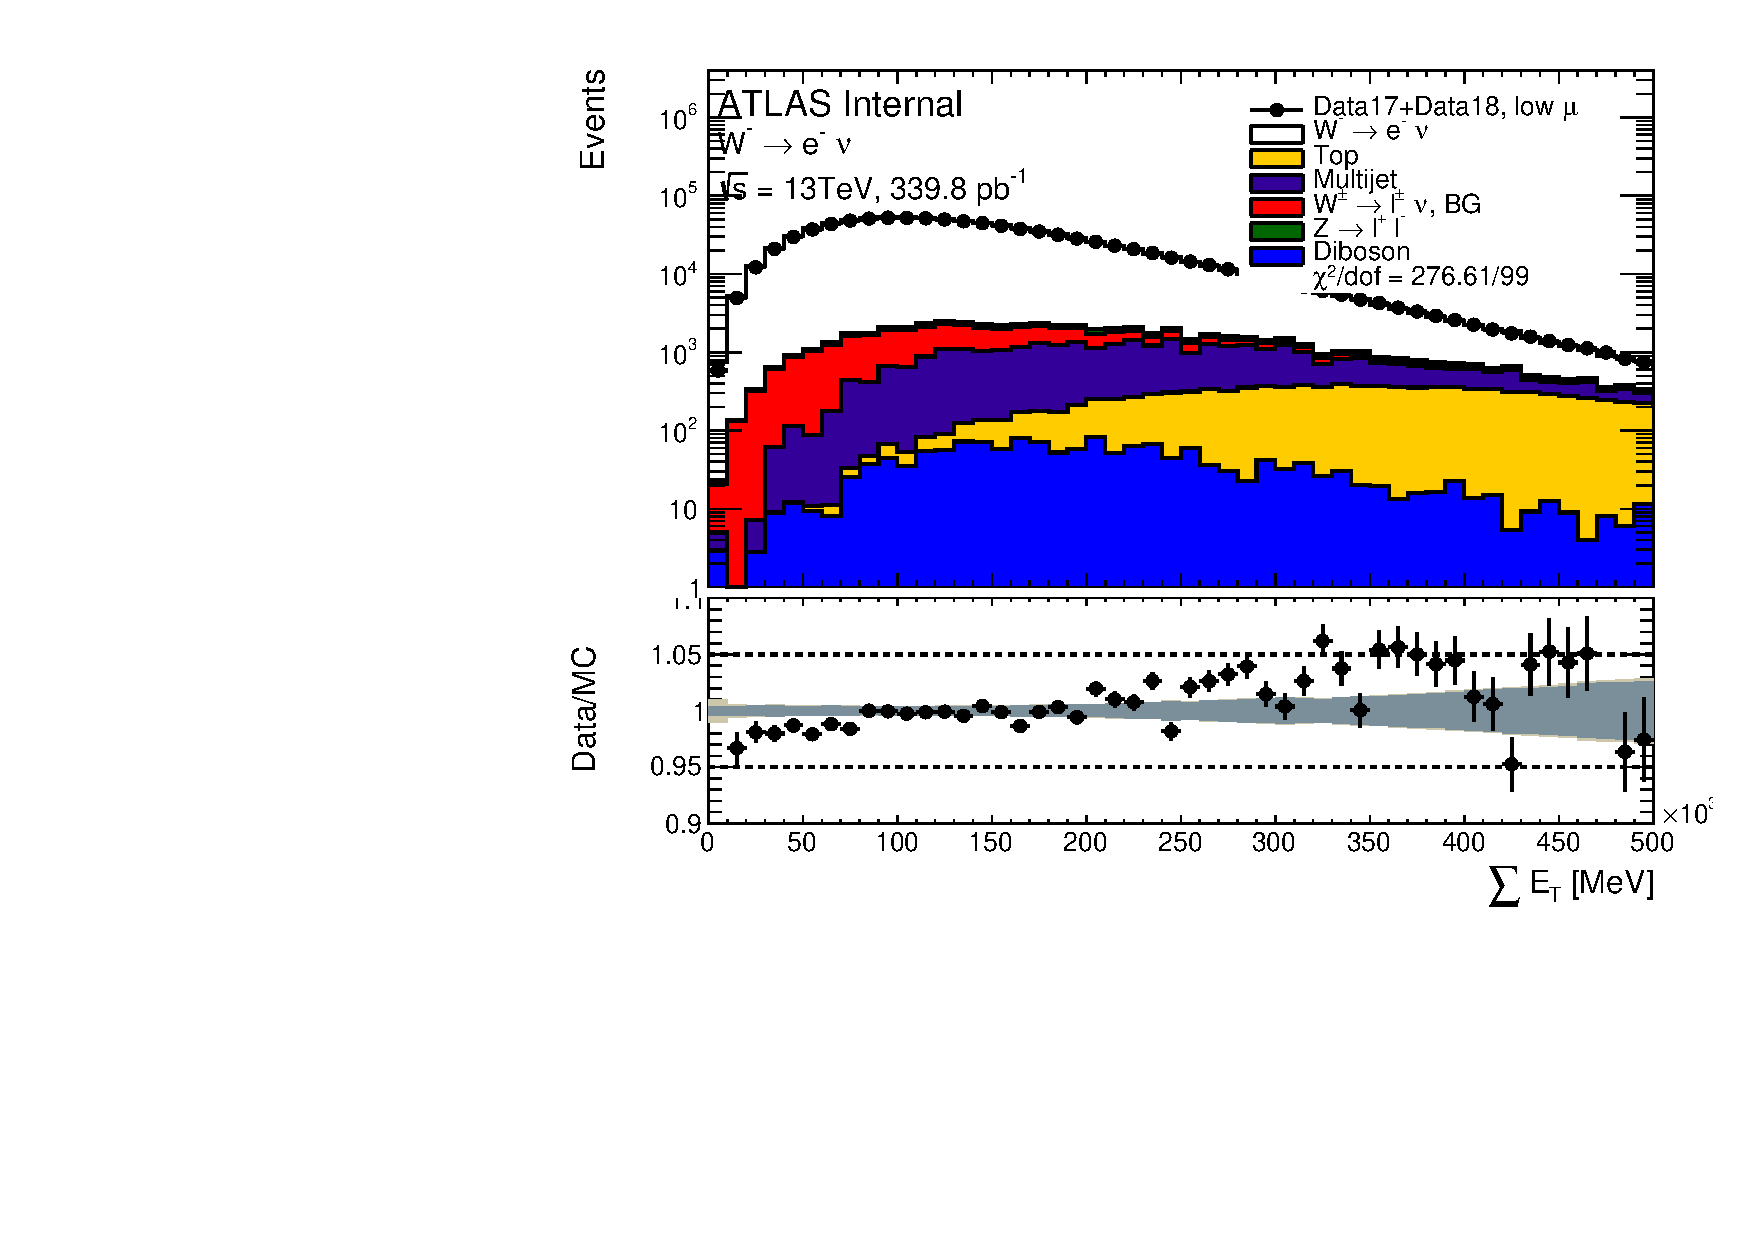
\includegraphics[width=.49\textwidth]{control_norm/SET_cut7_minusenu_13TeV_log_norm_NormErr.pdf}\label{f:}}
	{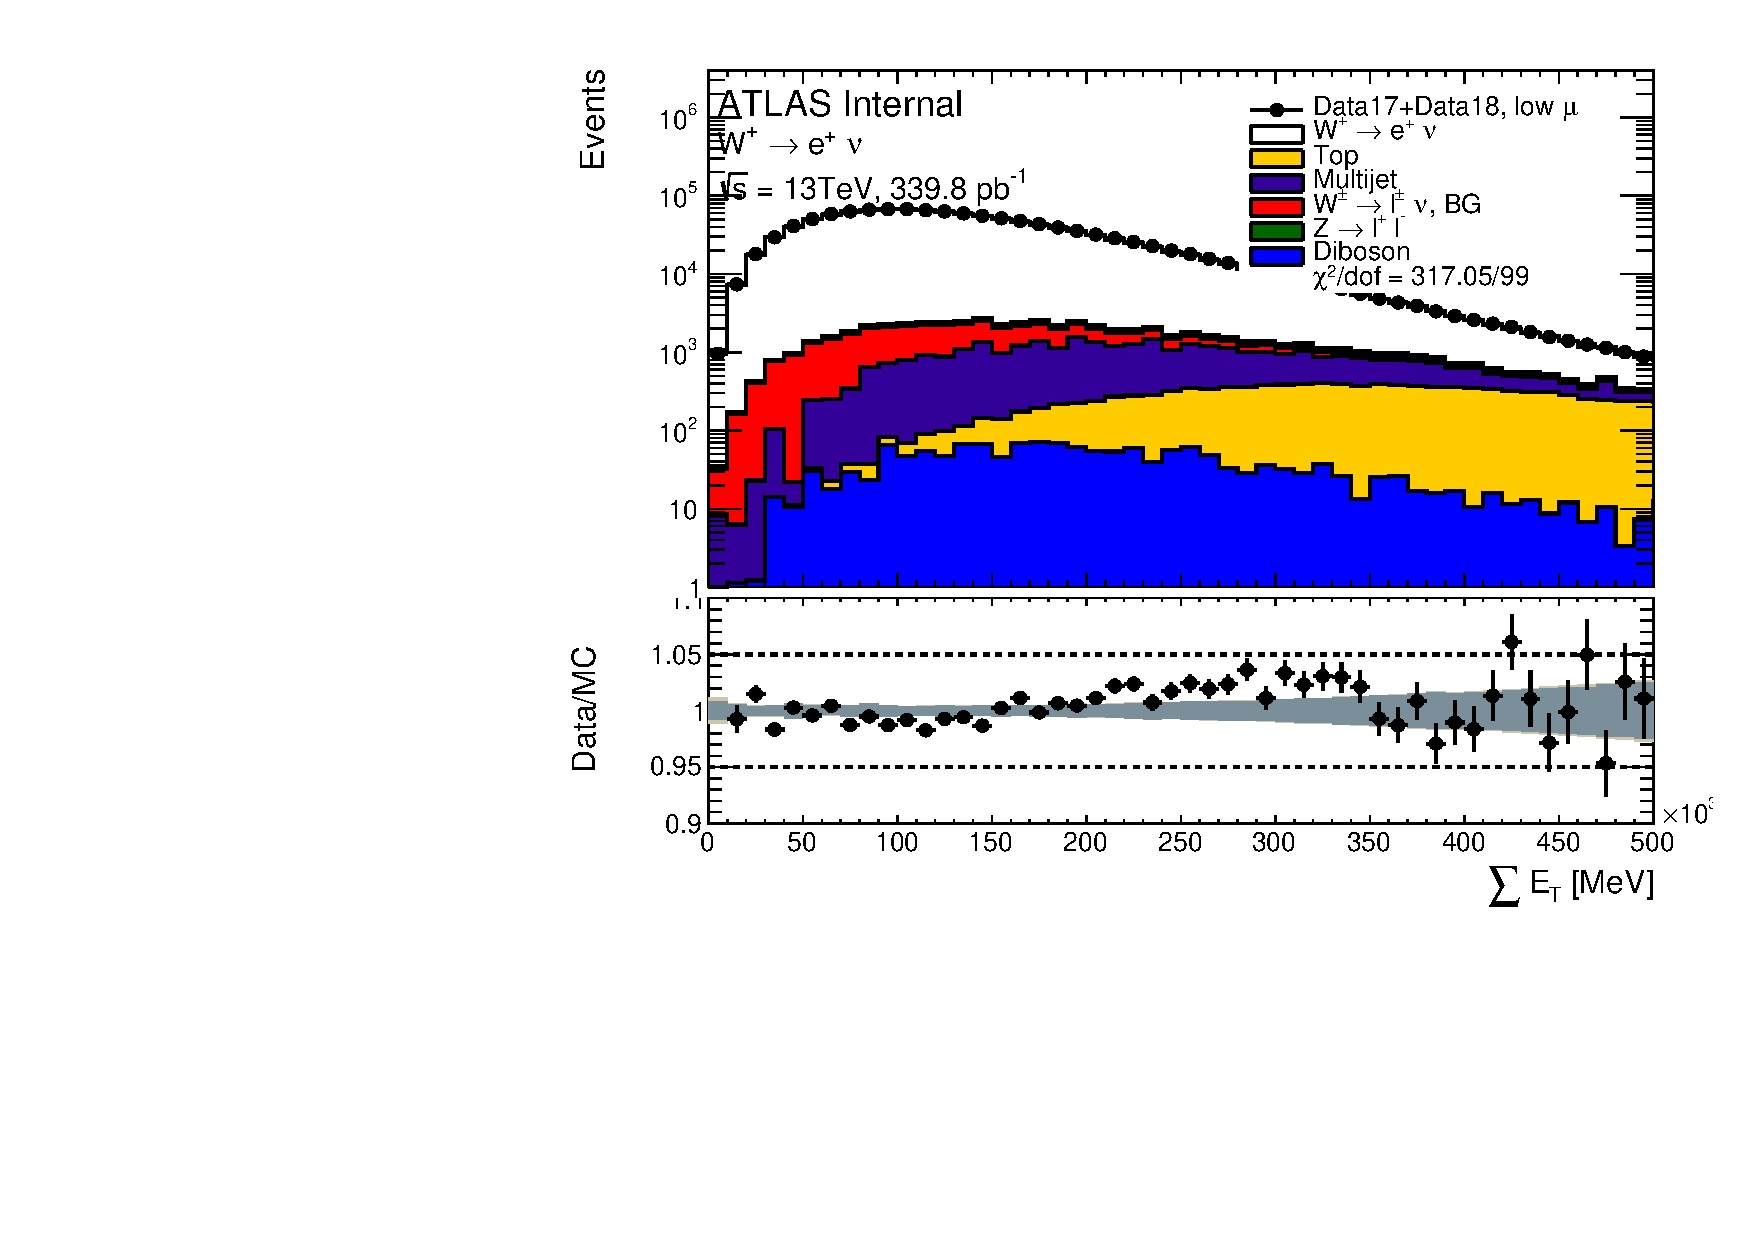
\includegraphics[width=.49\textwidth]{control_norm/SET_cut7_plusenu_13TeV_log_norm_NormErr.pdf}\label{f:}}
	\caption{$\Sigma{E_T}$ distribution in the muon and electron channel  for the $\sqrt{s} = 13$~\TeV\ dataset.}\end{figure}



\begin{figure}[h]
	\centering
	{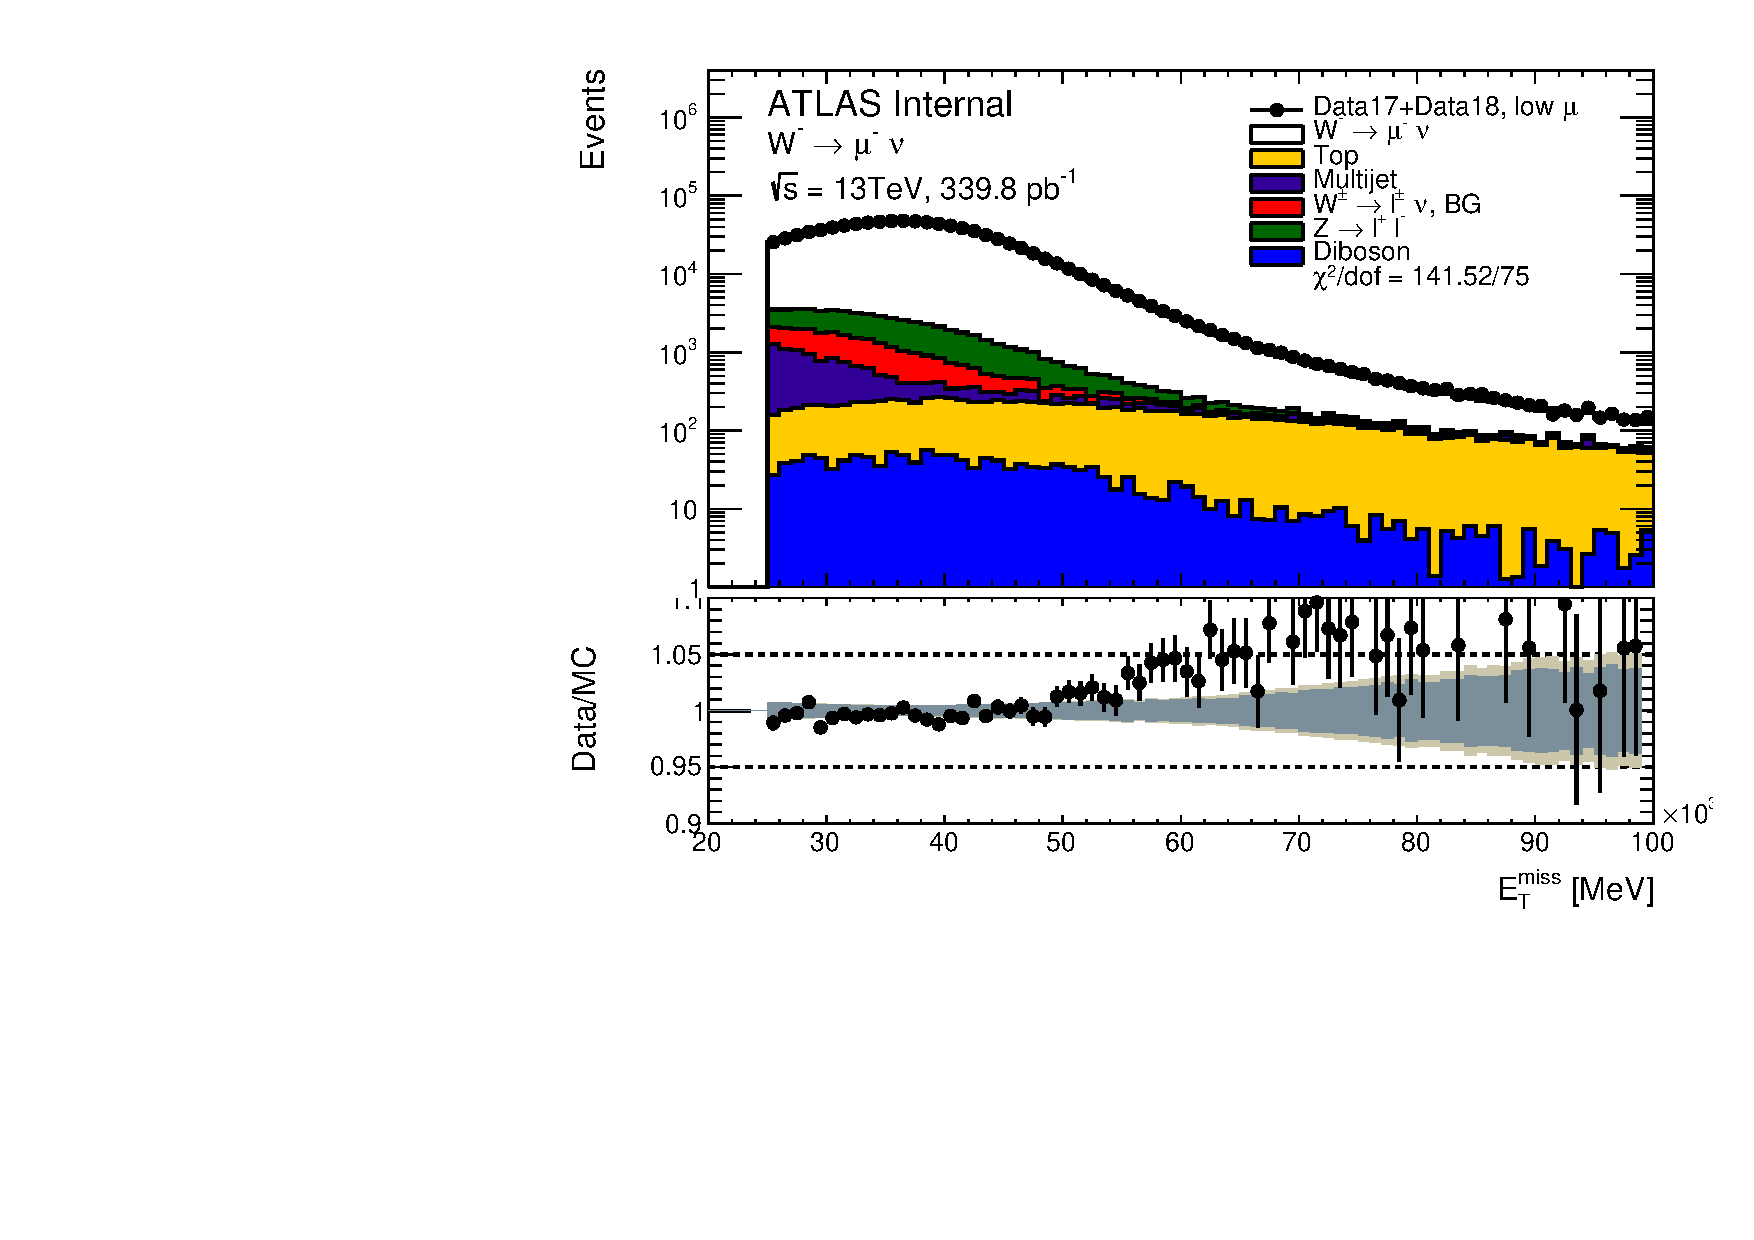
\includegraphics[width=.49\textwidth]{control_norm/met_cut7_minusmunu_13TeV_log_norm_NormErr.pdf}\label{f:}}
	{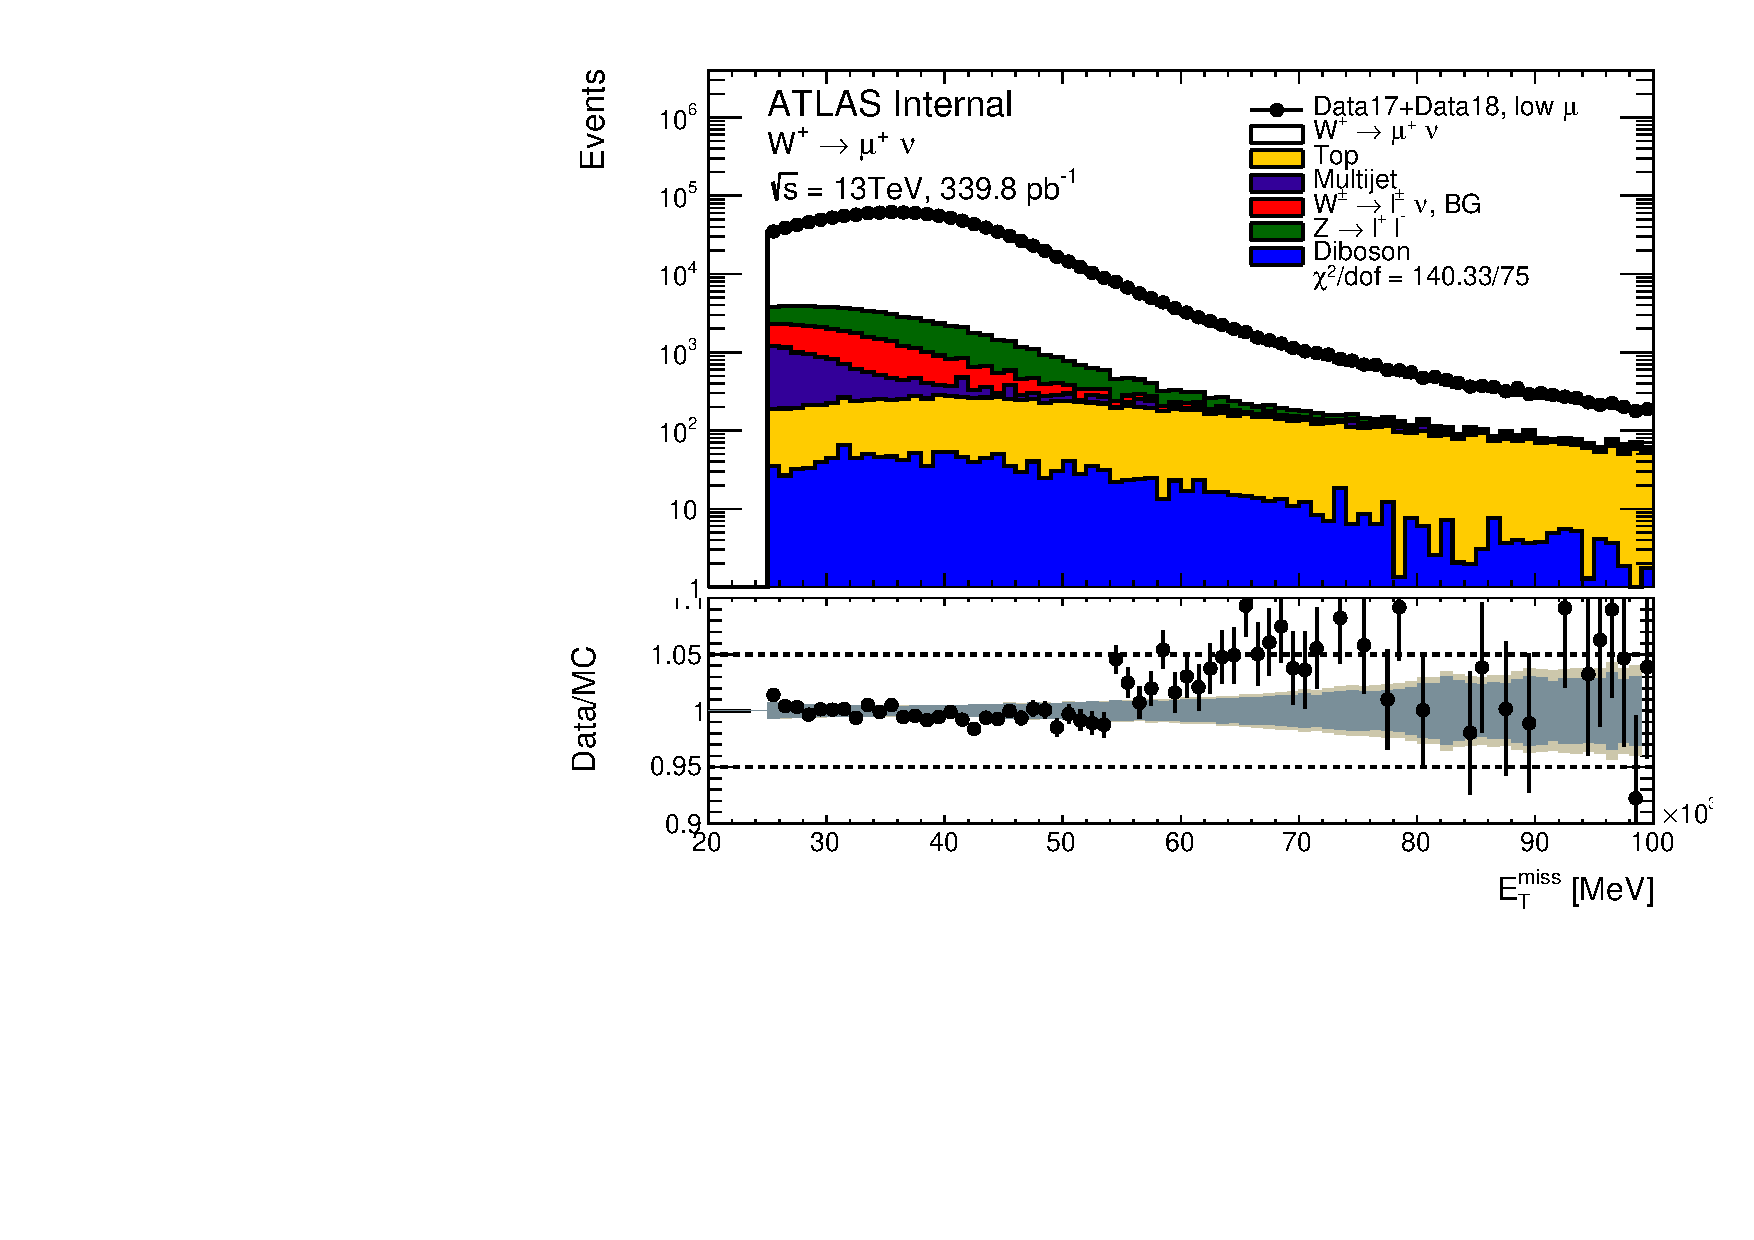
\includegraphics[width=.49\textwidth]{control_norm/met_cut7_plusmunu_13TeV_log_norm_NormErr.pdf}\label{f:}}
	
	{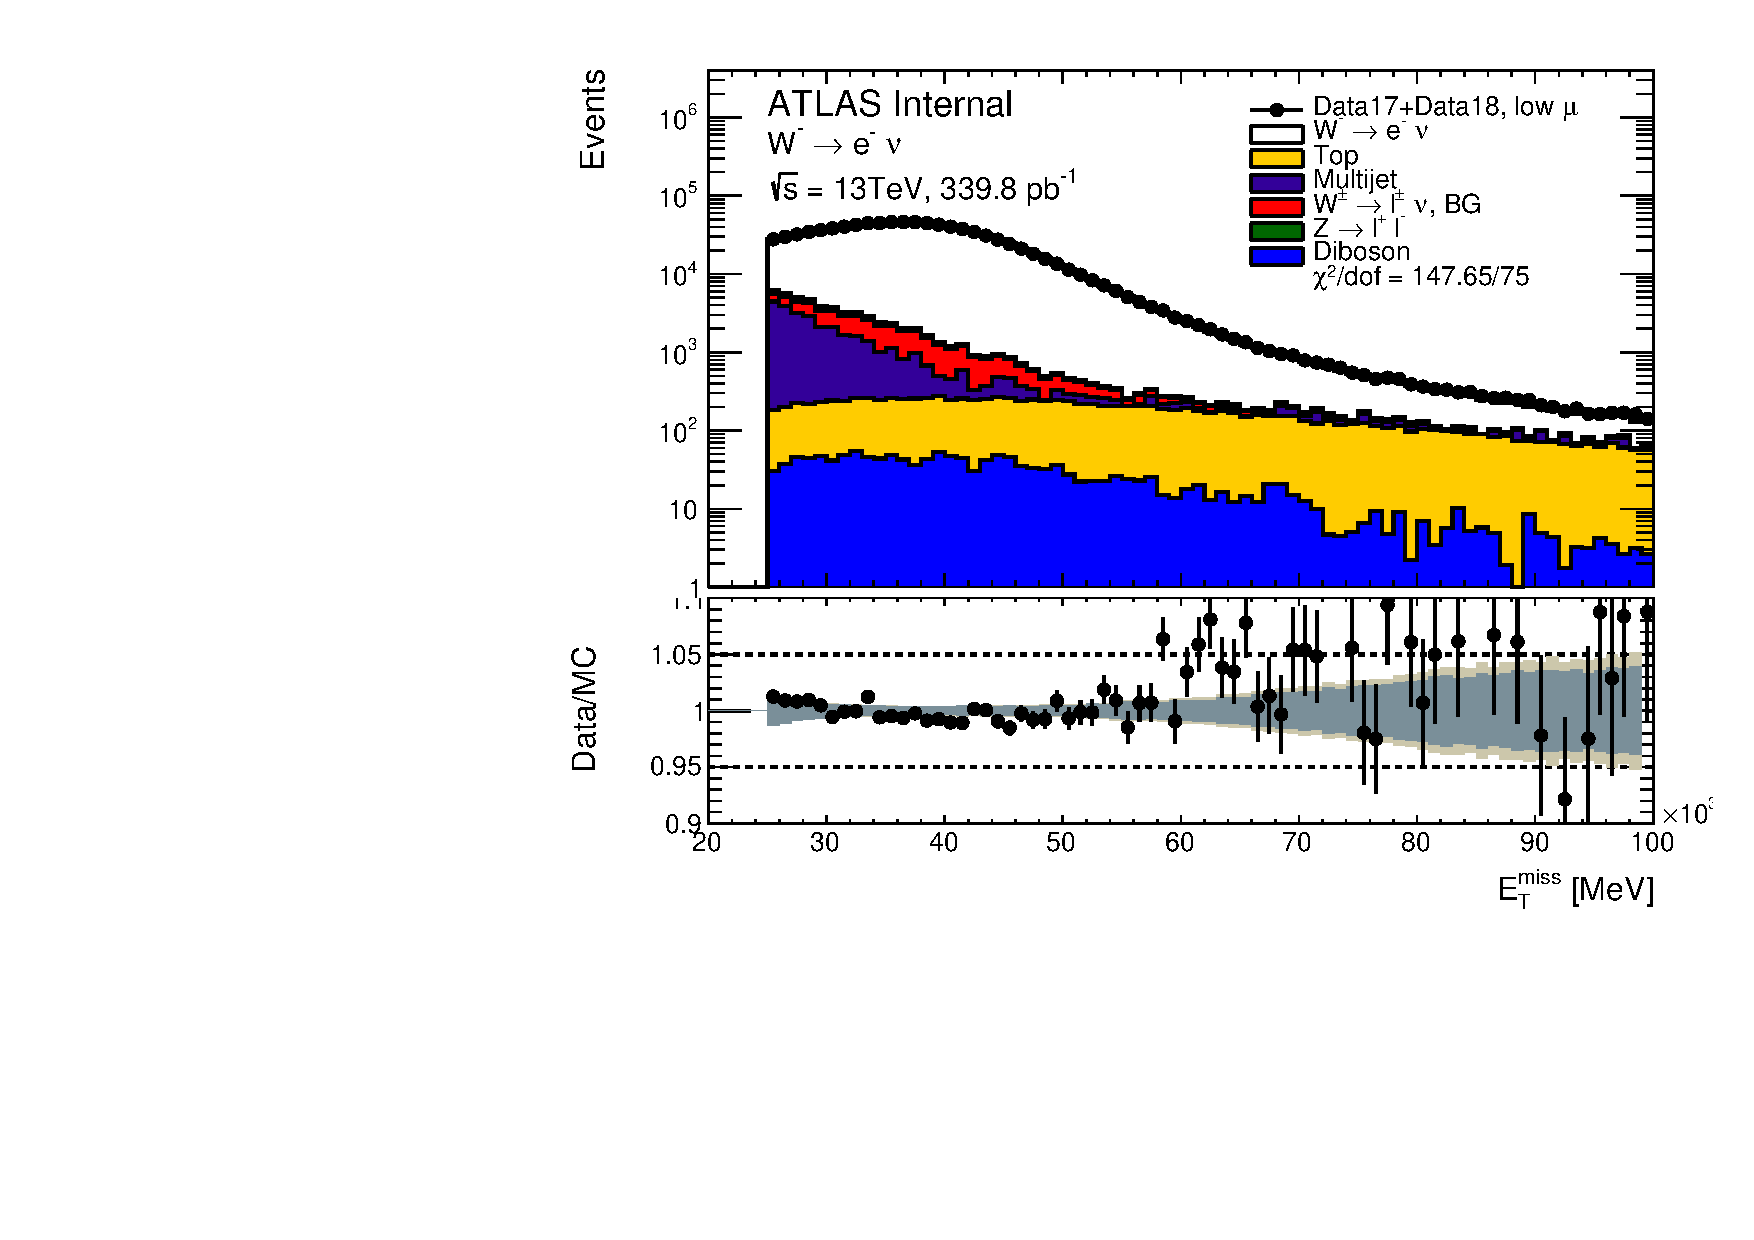
\includegraphics[width=.49\textwidth]{control_norm/met_cut7_minusenu_13TeV_log_norm_NormErr.pdf}\label{f:}}
	{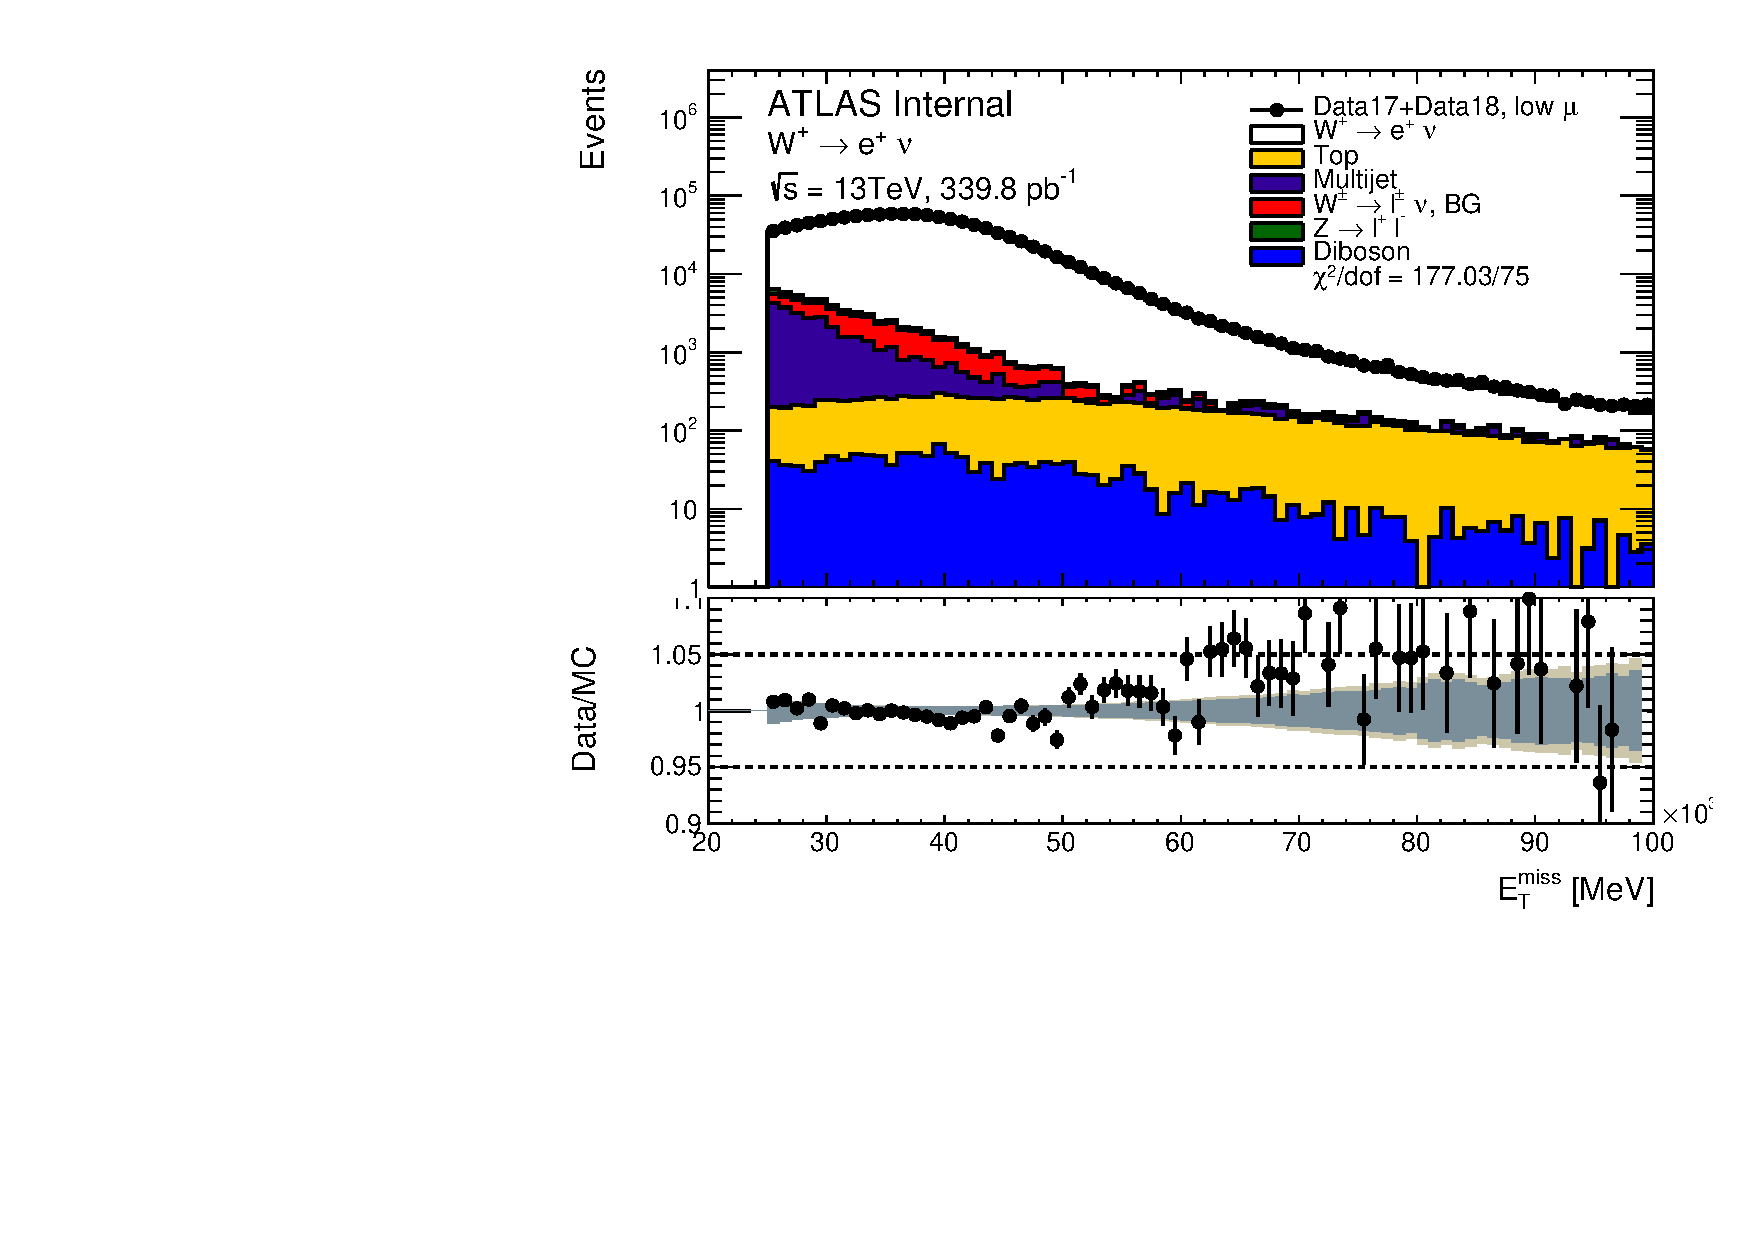
\includegraphics[width=.49\textwidth]{control_norm/met_cut7_plusenu_13TeV_log_norm_NormErr.pdf}\label{f:}}
	\caption{ $\vec{E}^{miss}_{T}$ distribution in the muon and electron channel  for the $\sqrt{s} = 13$~\TeV\ dataset. }\end{figure}




\begin{figure}[h]
	\centering
	{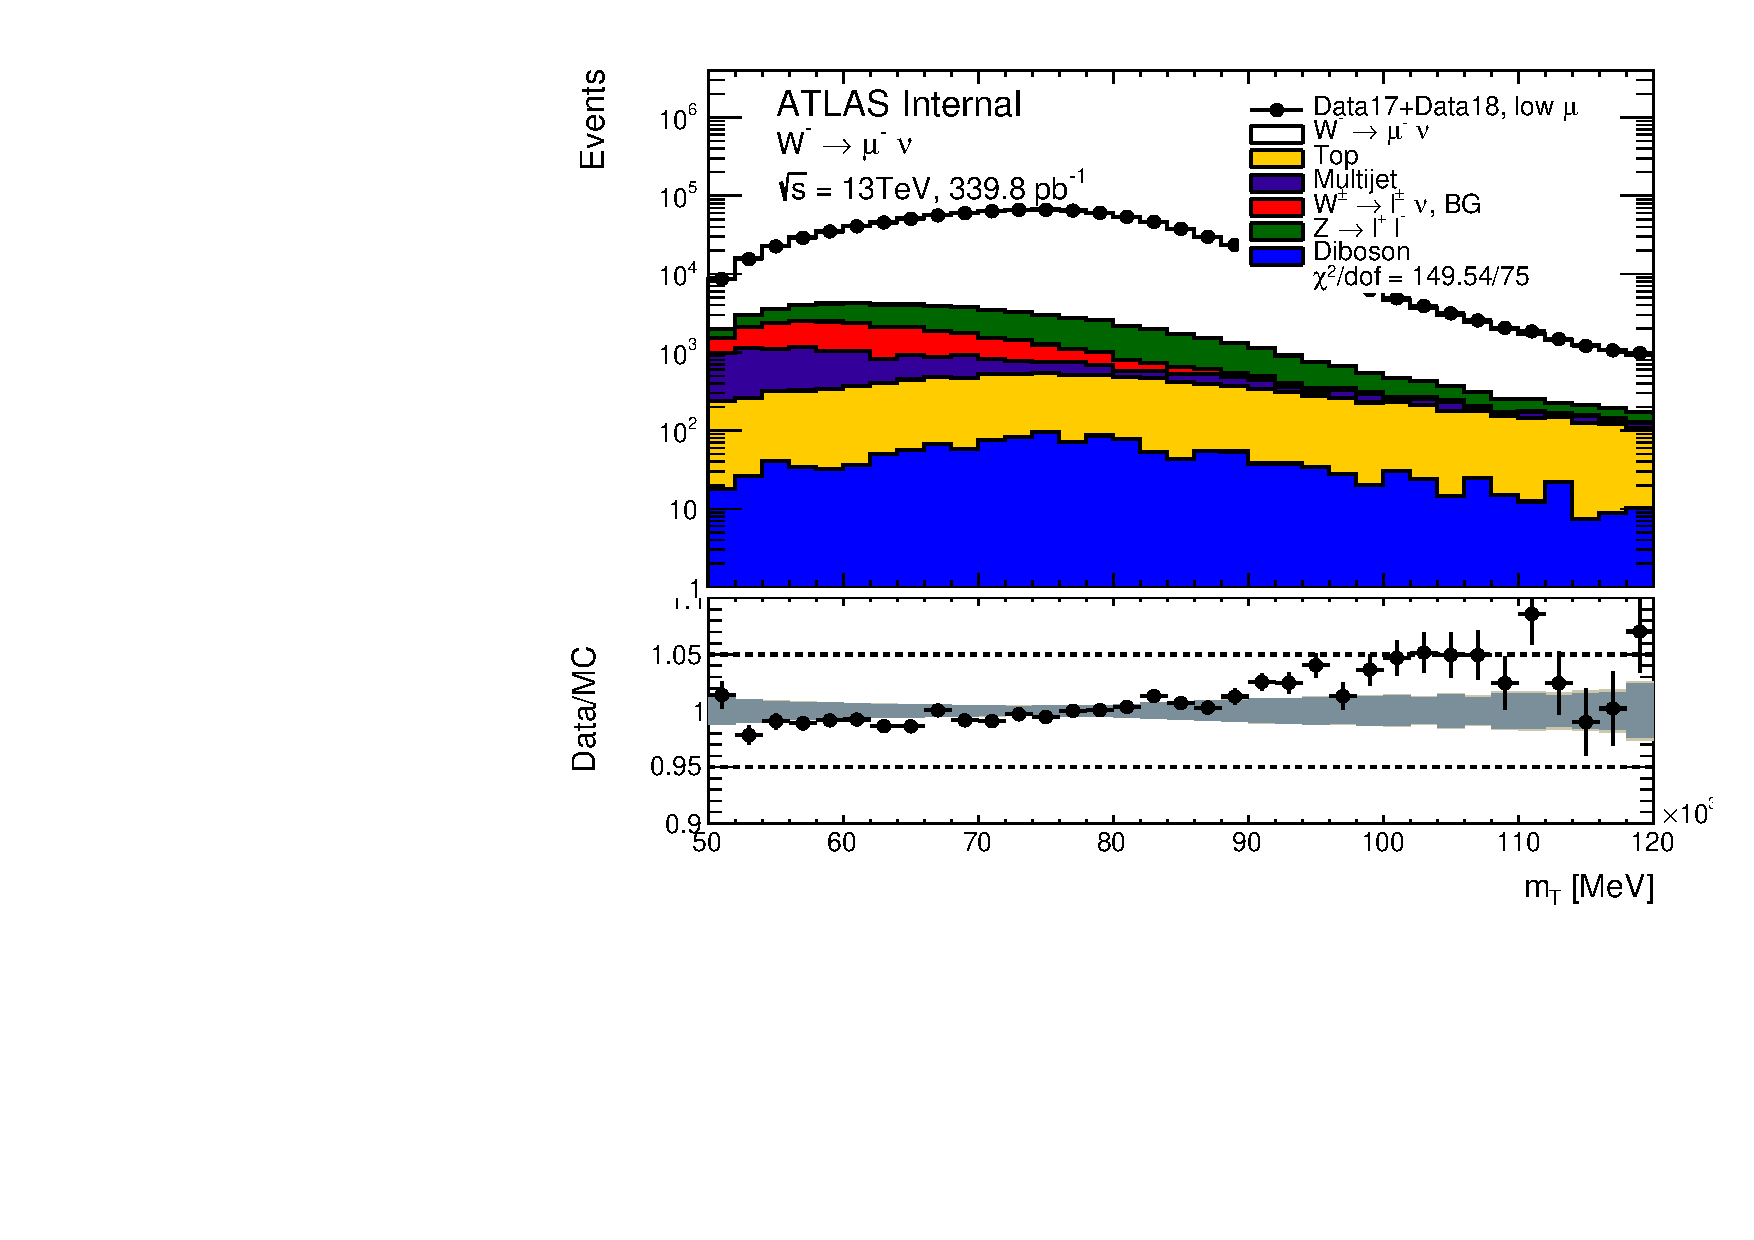
\includegraphics[width=.49\textwidth]{control_norm/mT_cut7_minusmunu_13TeV_log_norm_NormErr.pdf}\label{f:}}
	{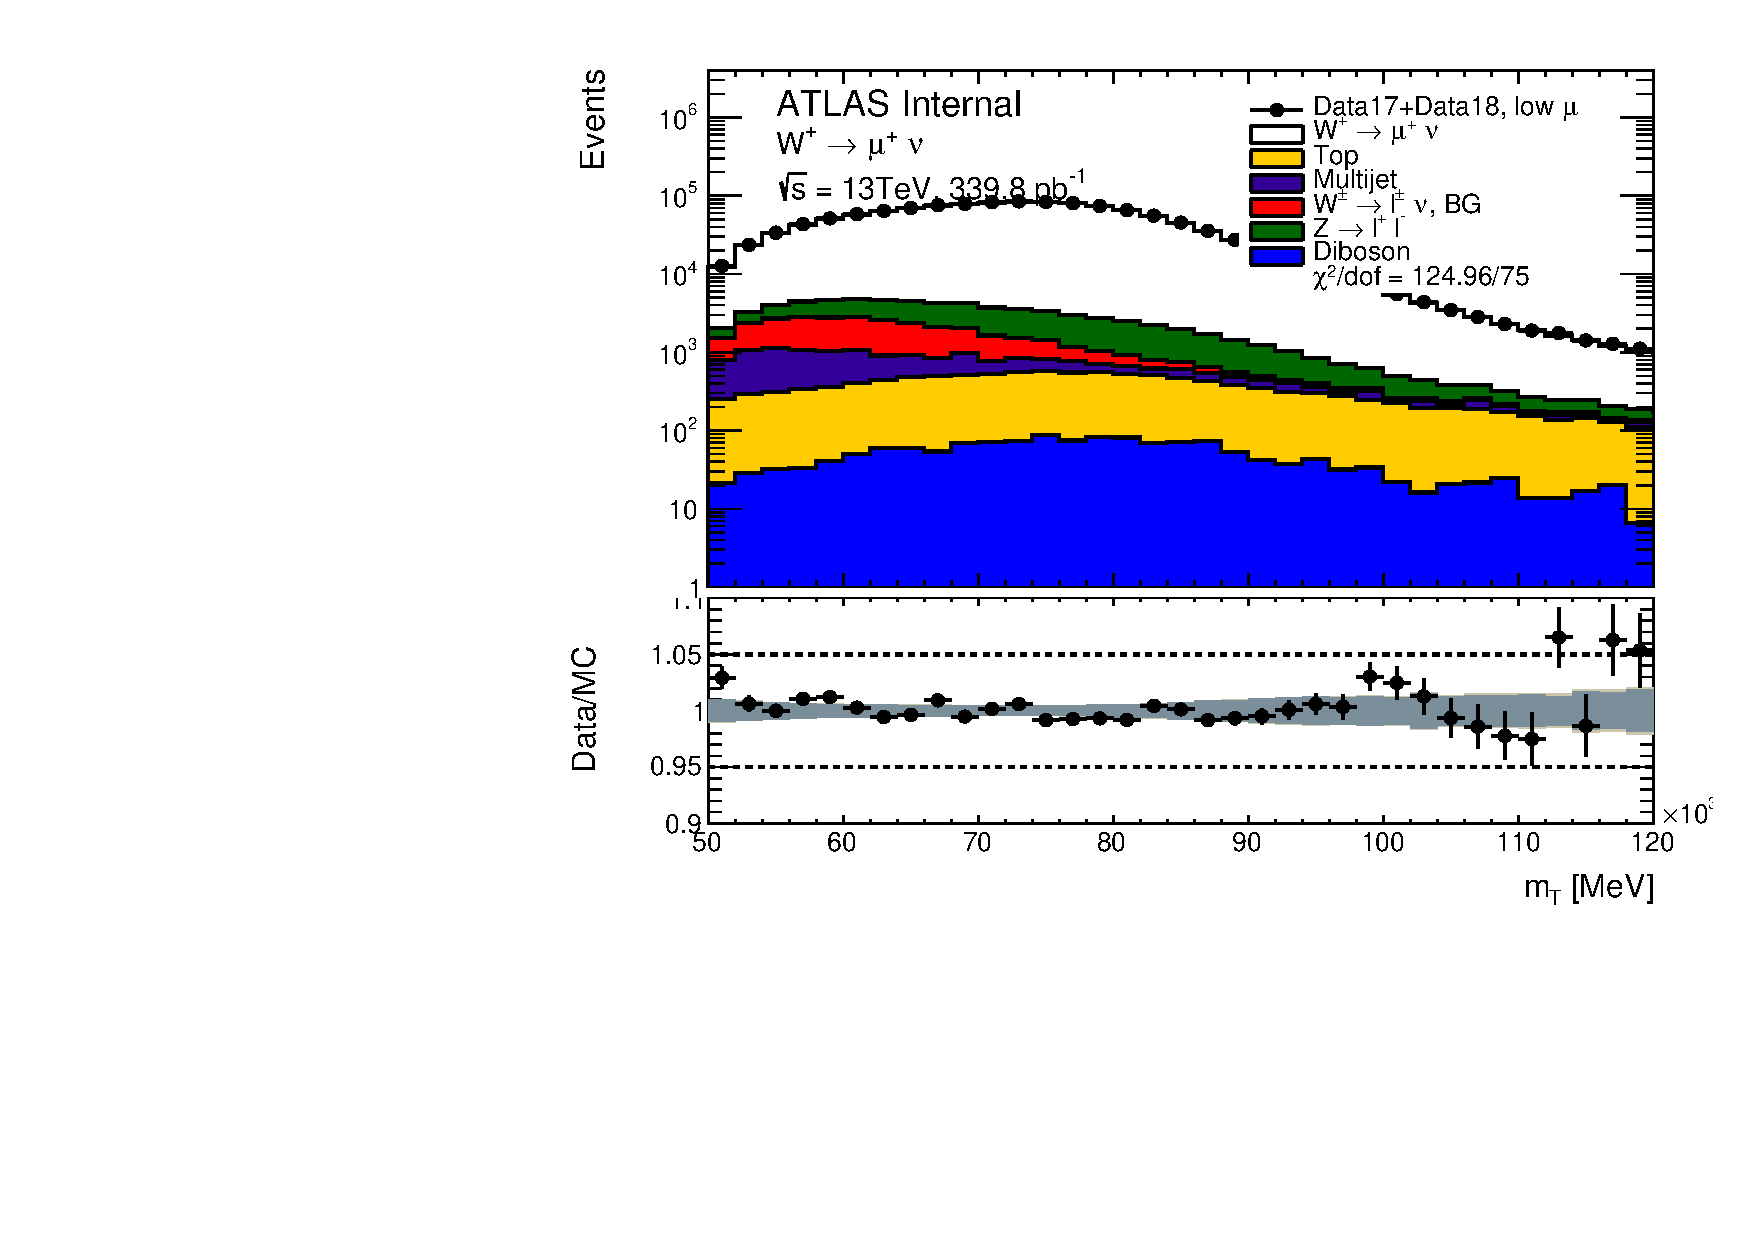
\includegraphics[width=.49\textwidth]{control_norm/mT_cut7_plusmunu_13TeV_log_norm_NormErr.pdf}\label{f:}}
	
	{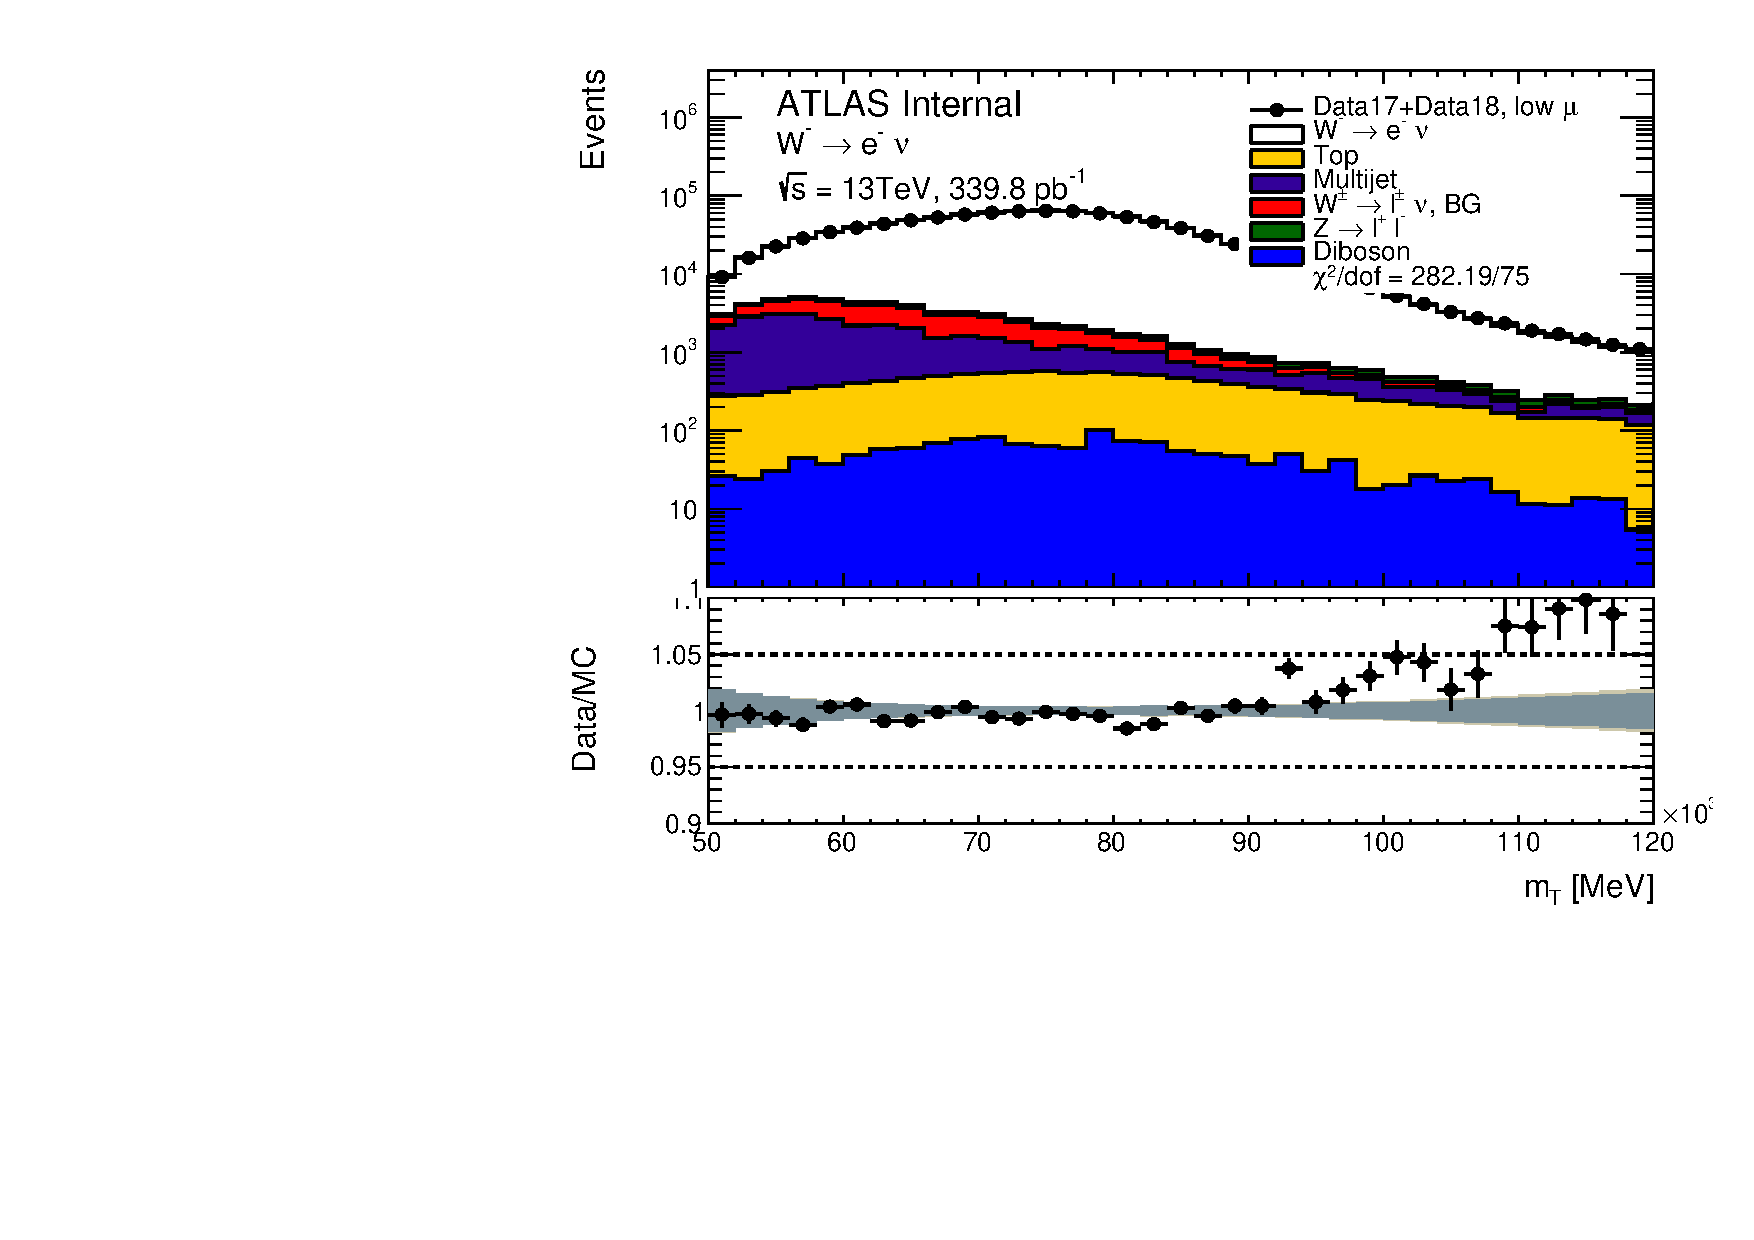
\includegraphics[width=.49\textwidth]{control_norm/mT_cut7_minusenu_13TeV_log_norm_NormErr.pdf}\label{f:}}
	{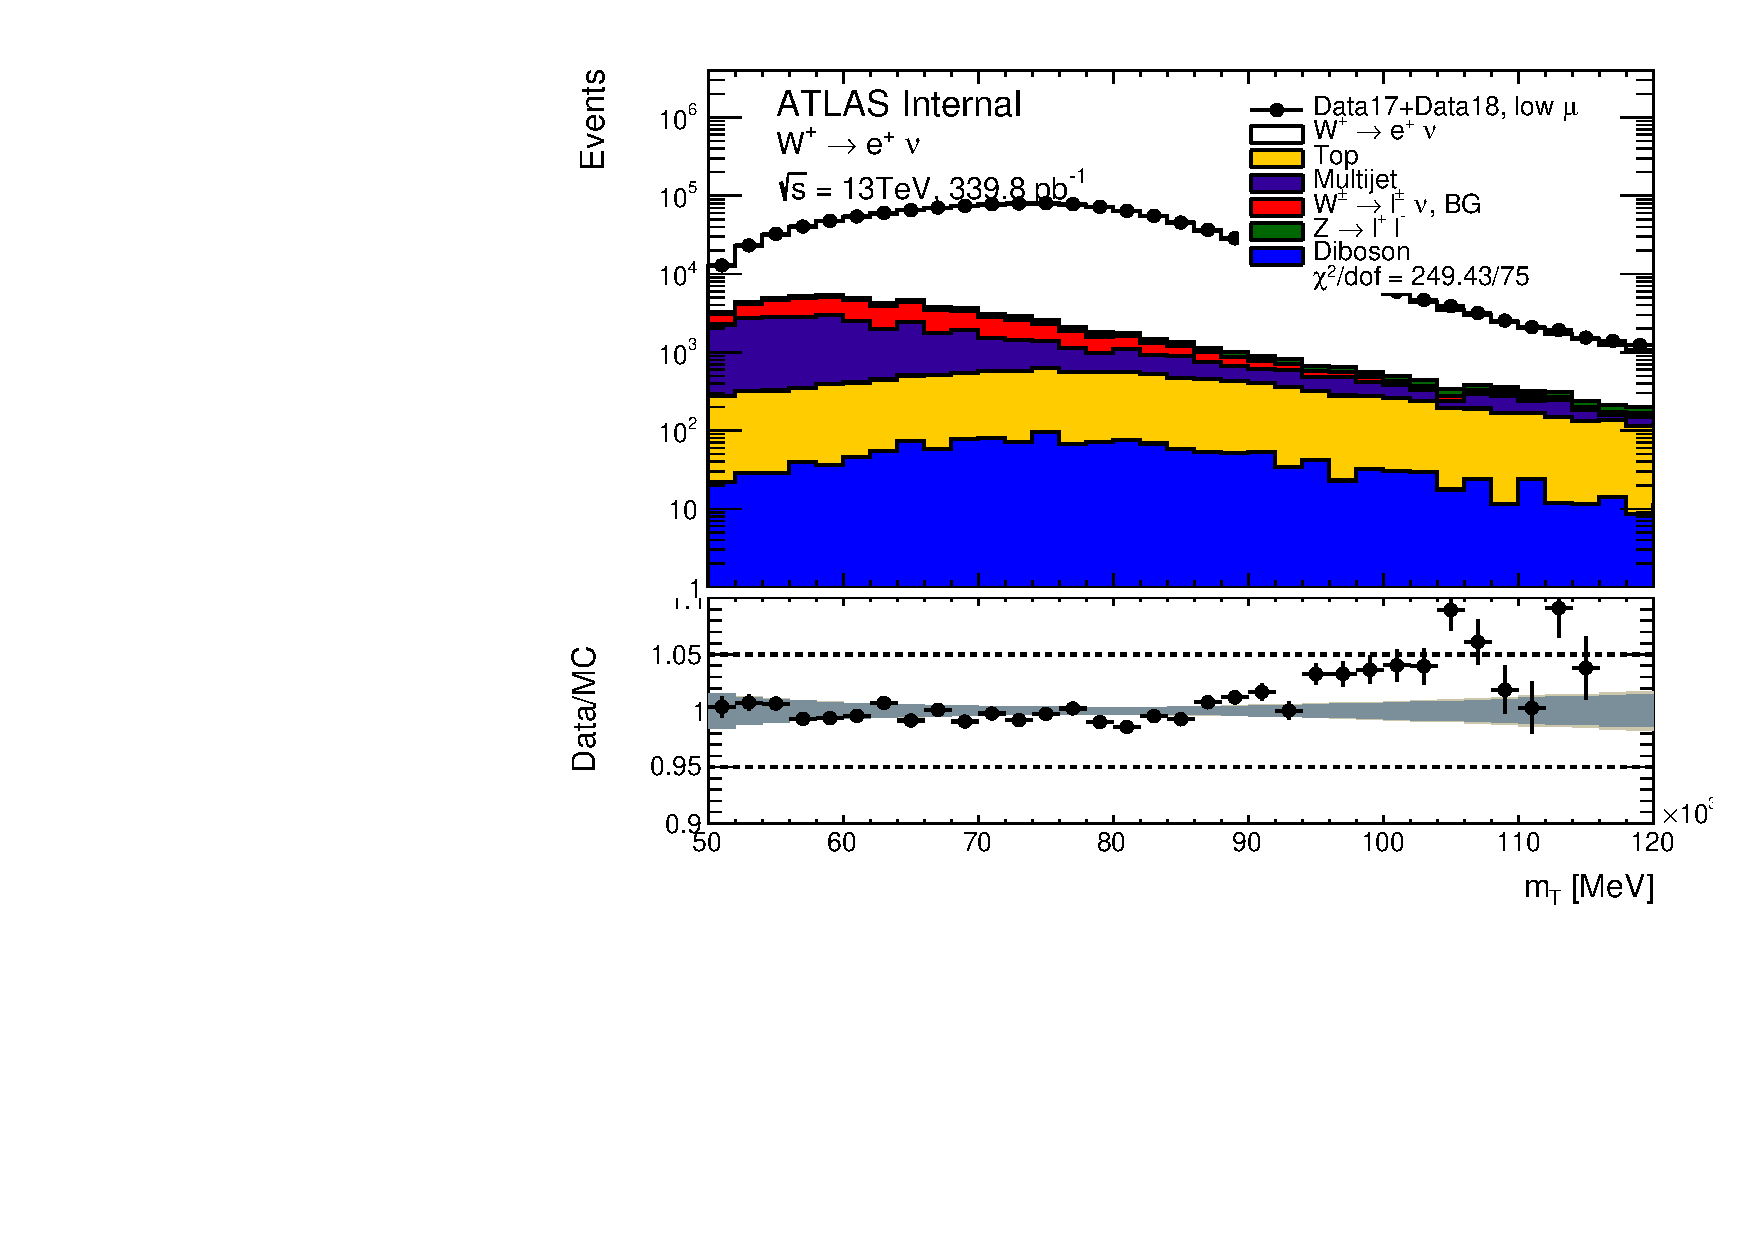
\includegraphics[width=.49\textwidth]{control_norm/mT_cut7_plusenu_13TeV_log_norm_NormErr.pdf}\label{f:}}
	\caption{  Transverse mass distribution of the W boson in the muon and electron channel  for the $\sqrt{s} = 13$~\TeV\ dataset. }\end{figure}


\begin{figure}[h]
	\centering
	{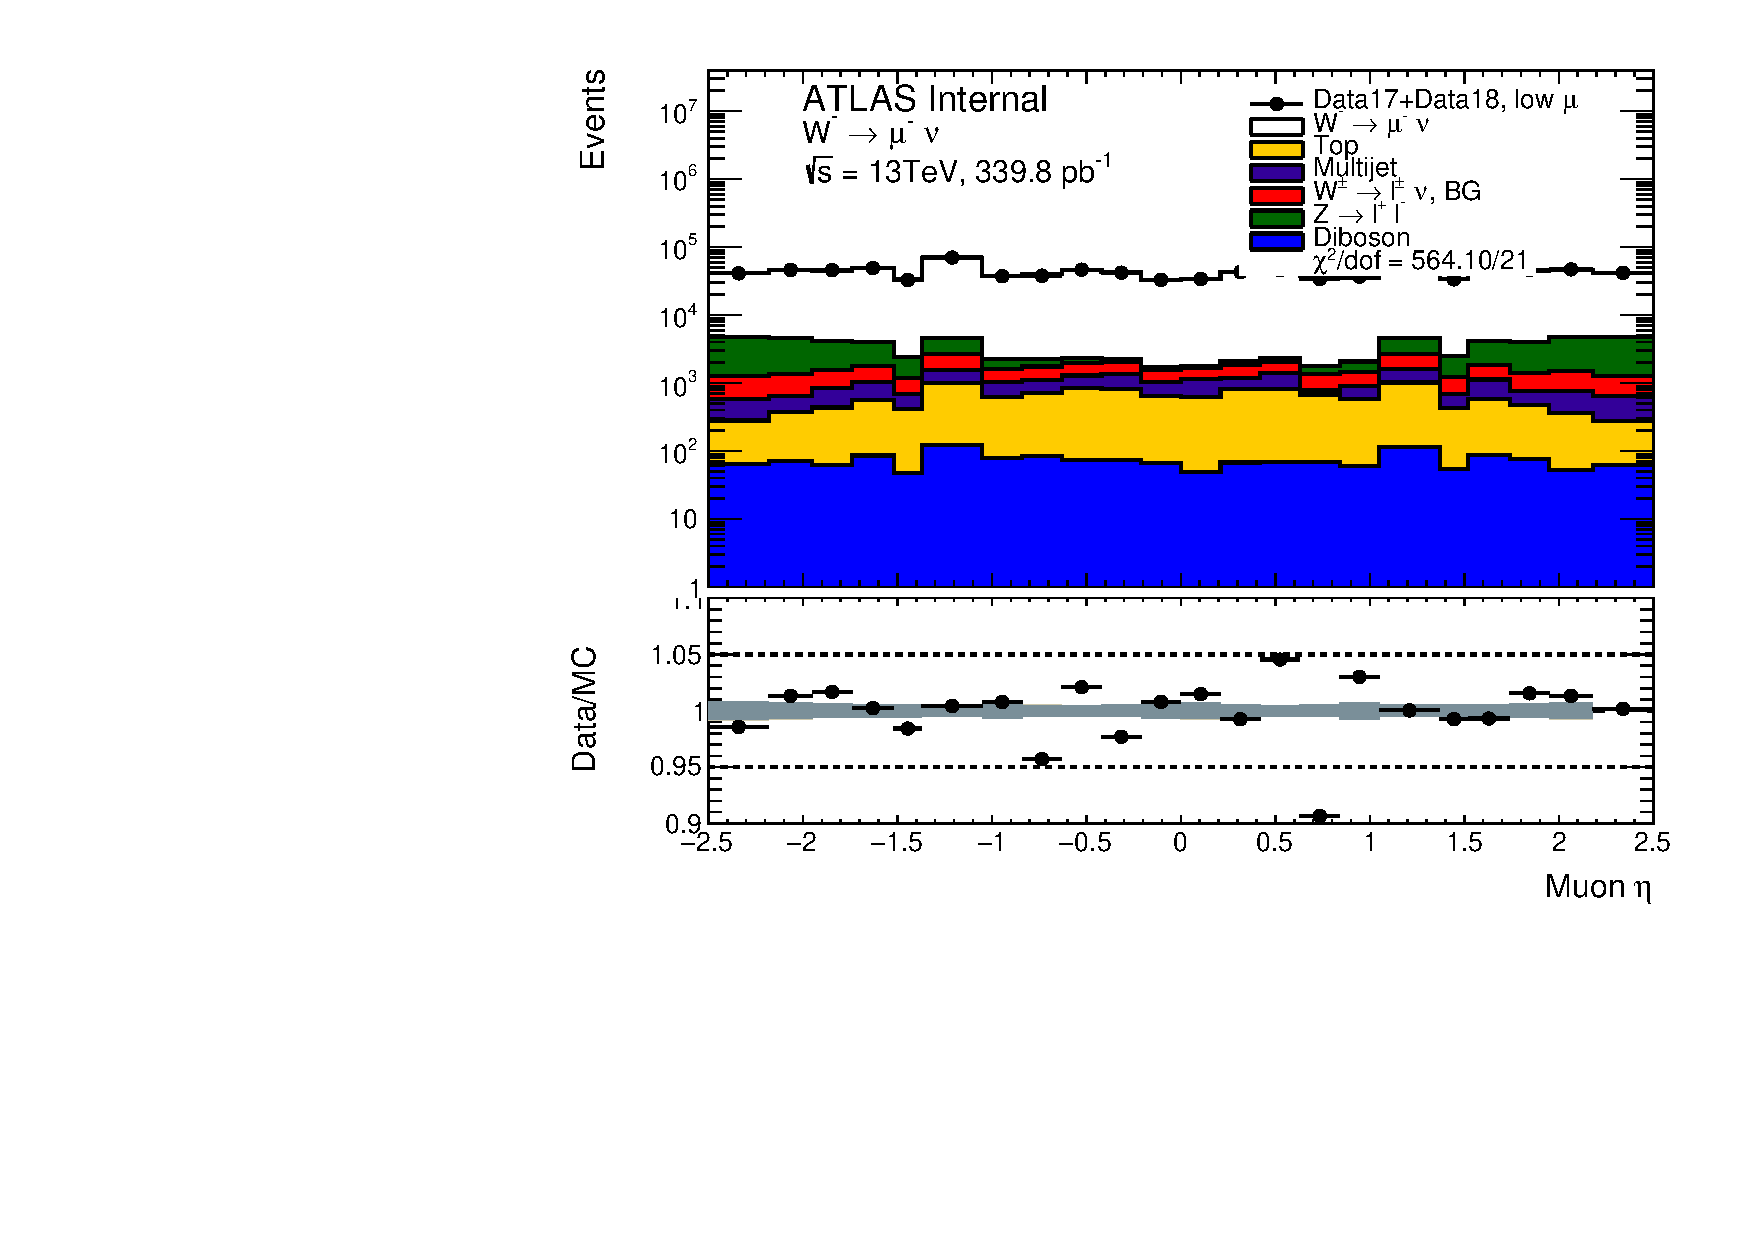
\includegraphics[width=.49\textwidth]{control_norm/muEta_cut7_minusmunu_13TeV_log_norm_NormErr.pdf}\label{f:}}
	{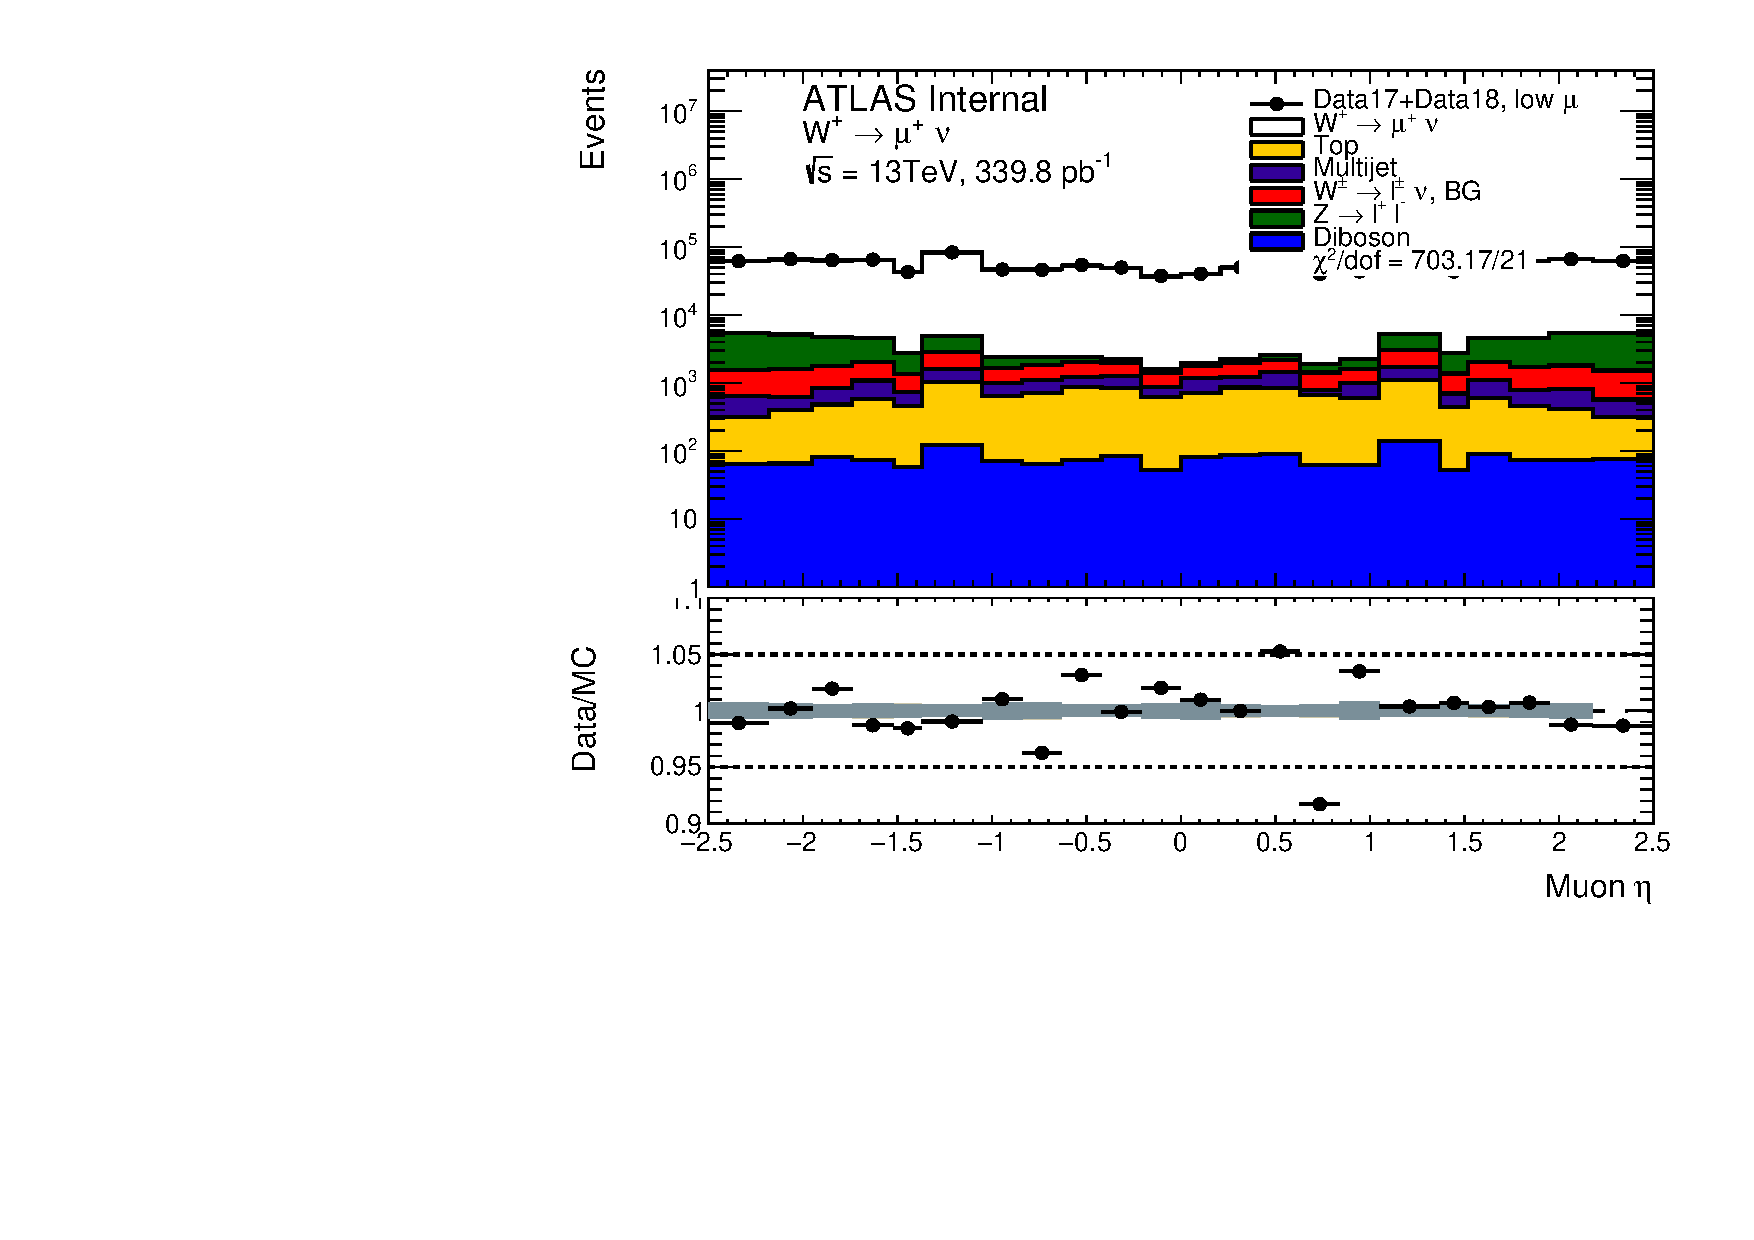
\includegraphics[width=.49\textwidth]{control_norm/muEta_cut7_plusmunu_13TeV_log_norm_NormErr.pdf}\label{f:}}
	
	{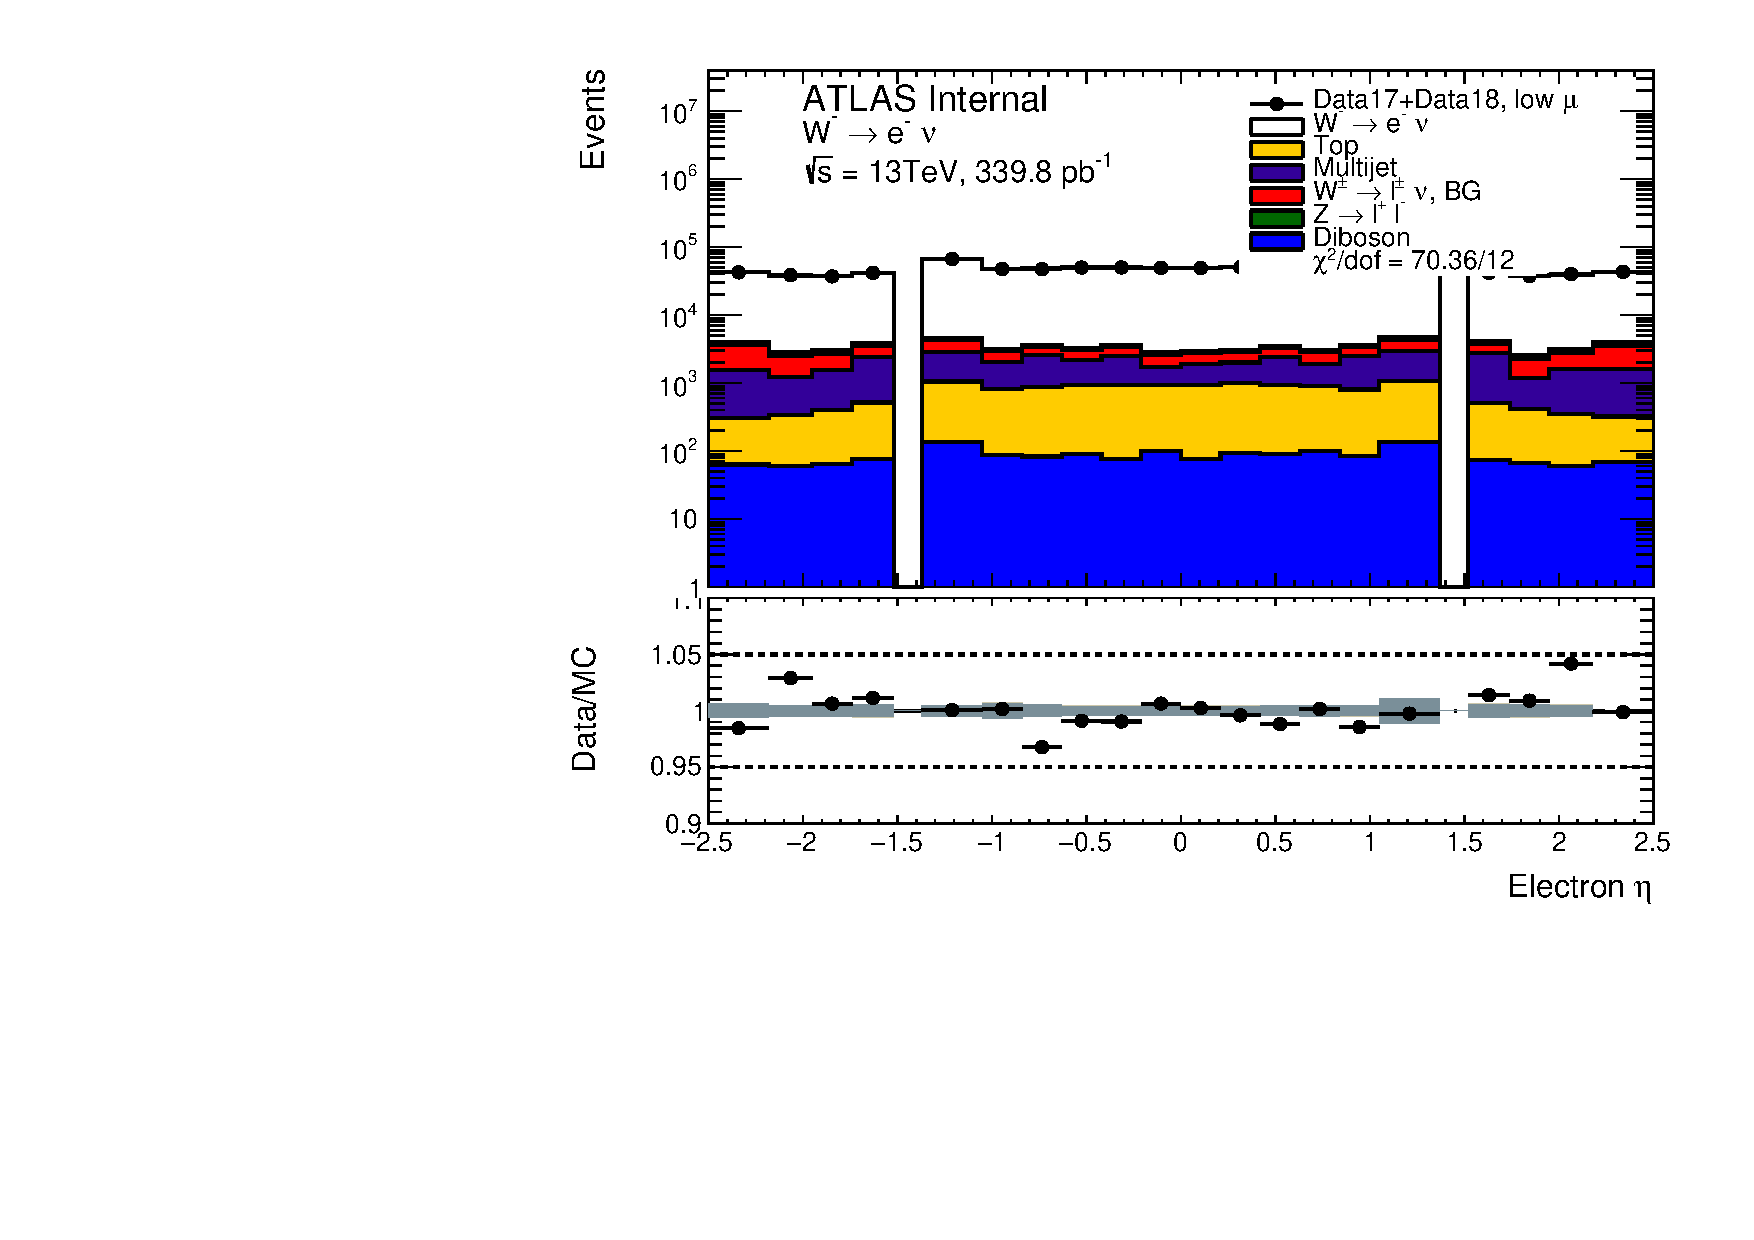
\includegraphics[width=.49\textwidth]{control_norm/elEta_cut7_minusenu_13TeV_log_norm_NormErr.pdf}\label{f:}}
	{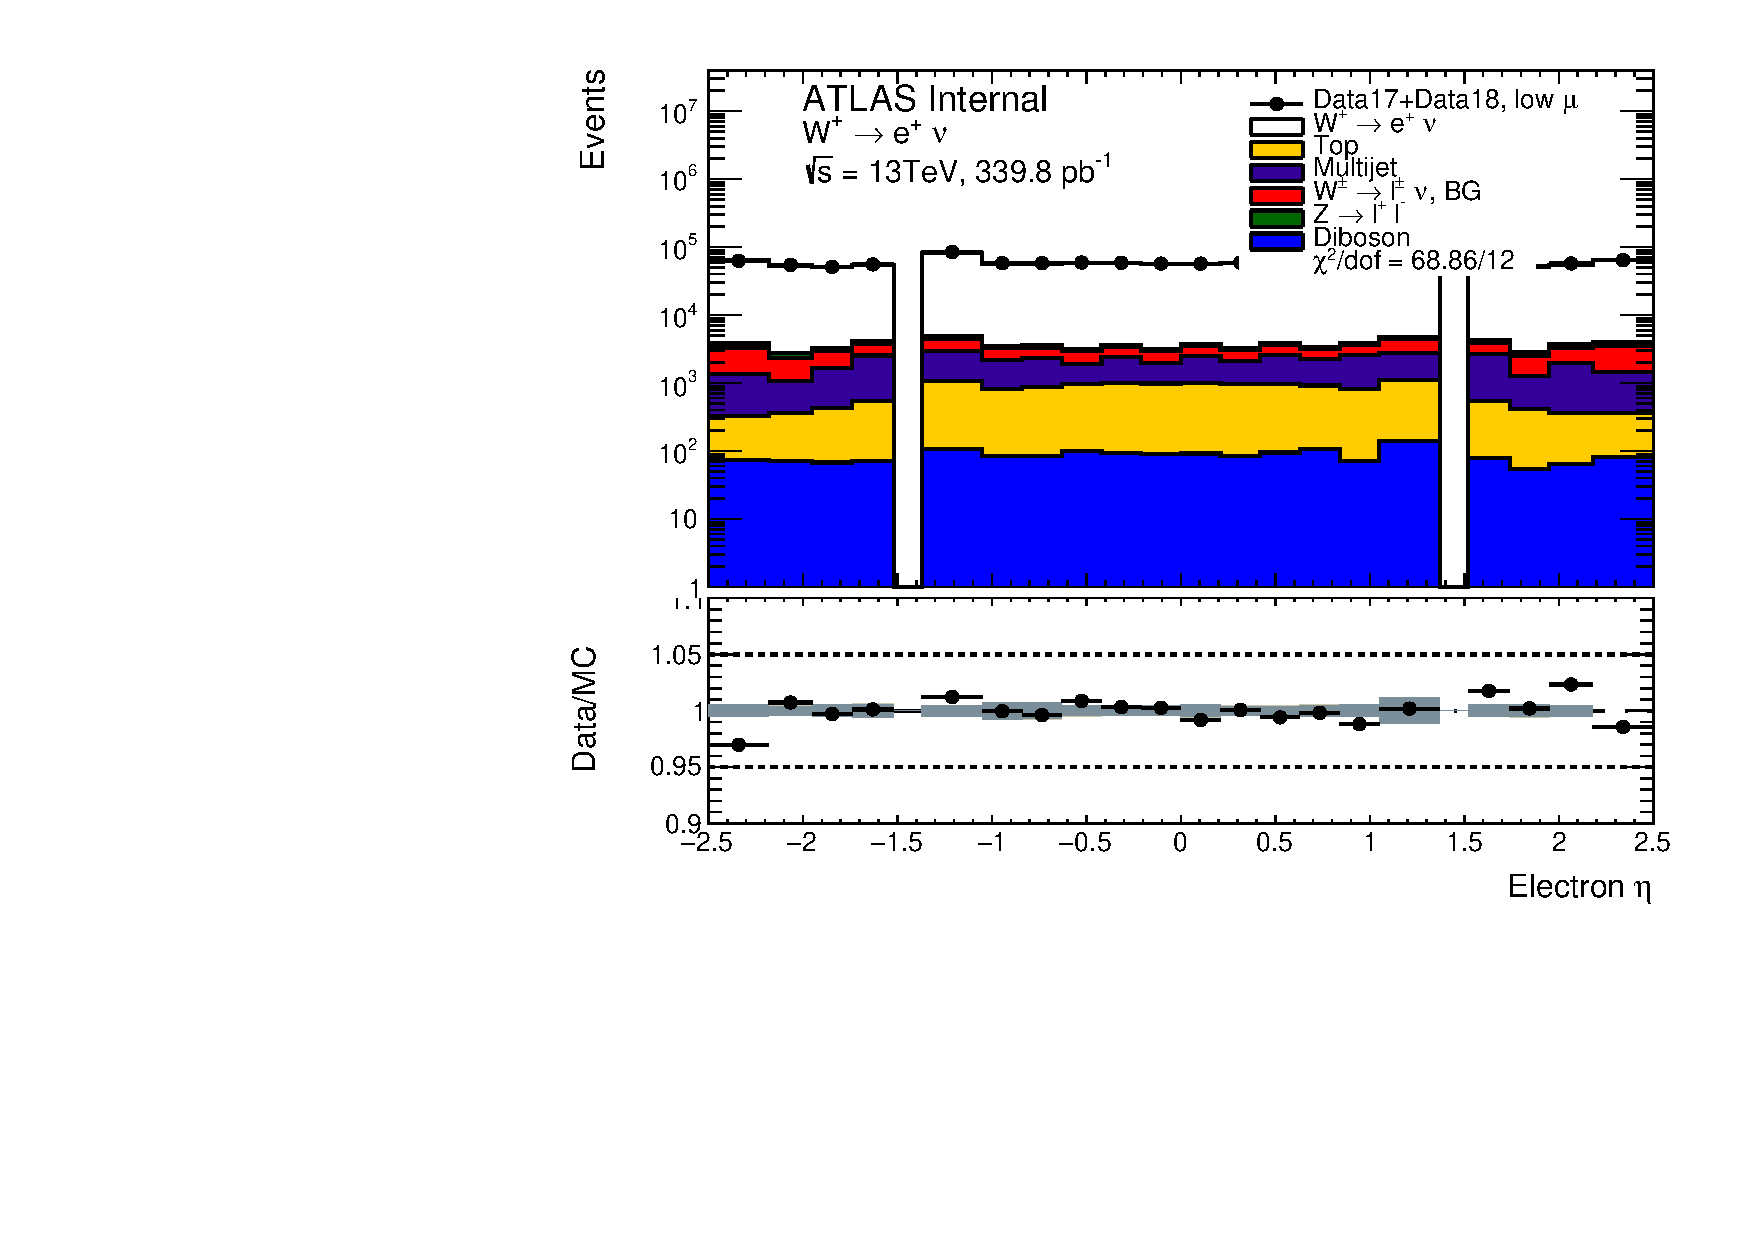
\includegraphics[width=.49\textwidth]{control_norm/elEta_cut7_plusenu_13TeV_log_norm_NormErr.pdf}\label{f:}}
	\caption{  Lepton pseudorapidity distribution in the muon and electron channel  for the $\sqrt{s} = 13$~\TeV\ dataset. }\end{figure}


\begin{figure}[h]
	\centering
	{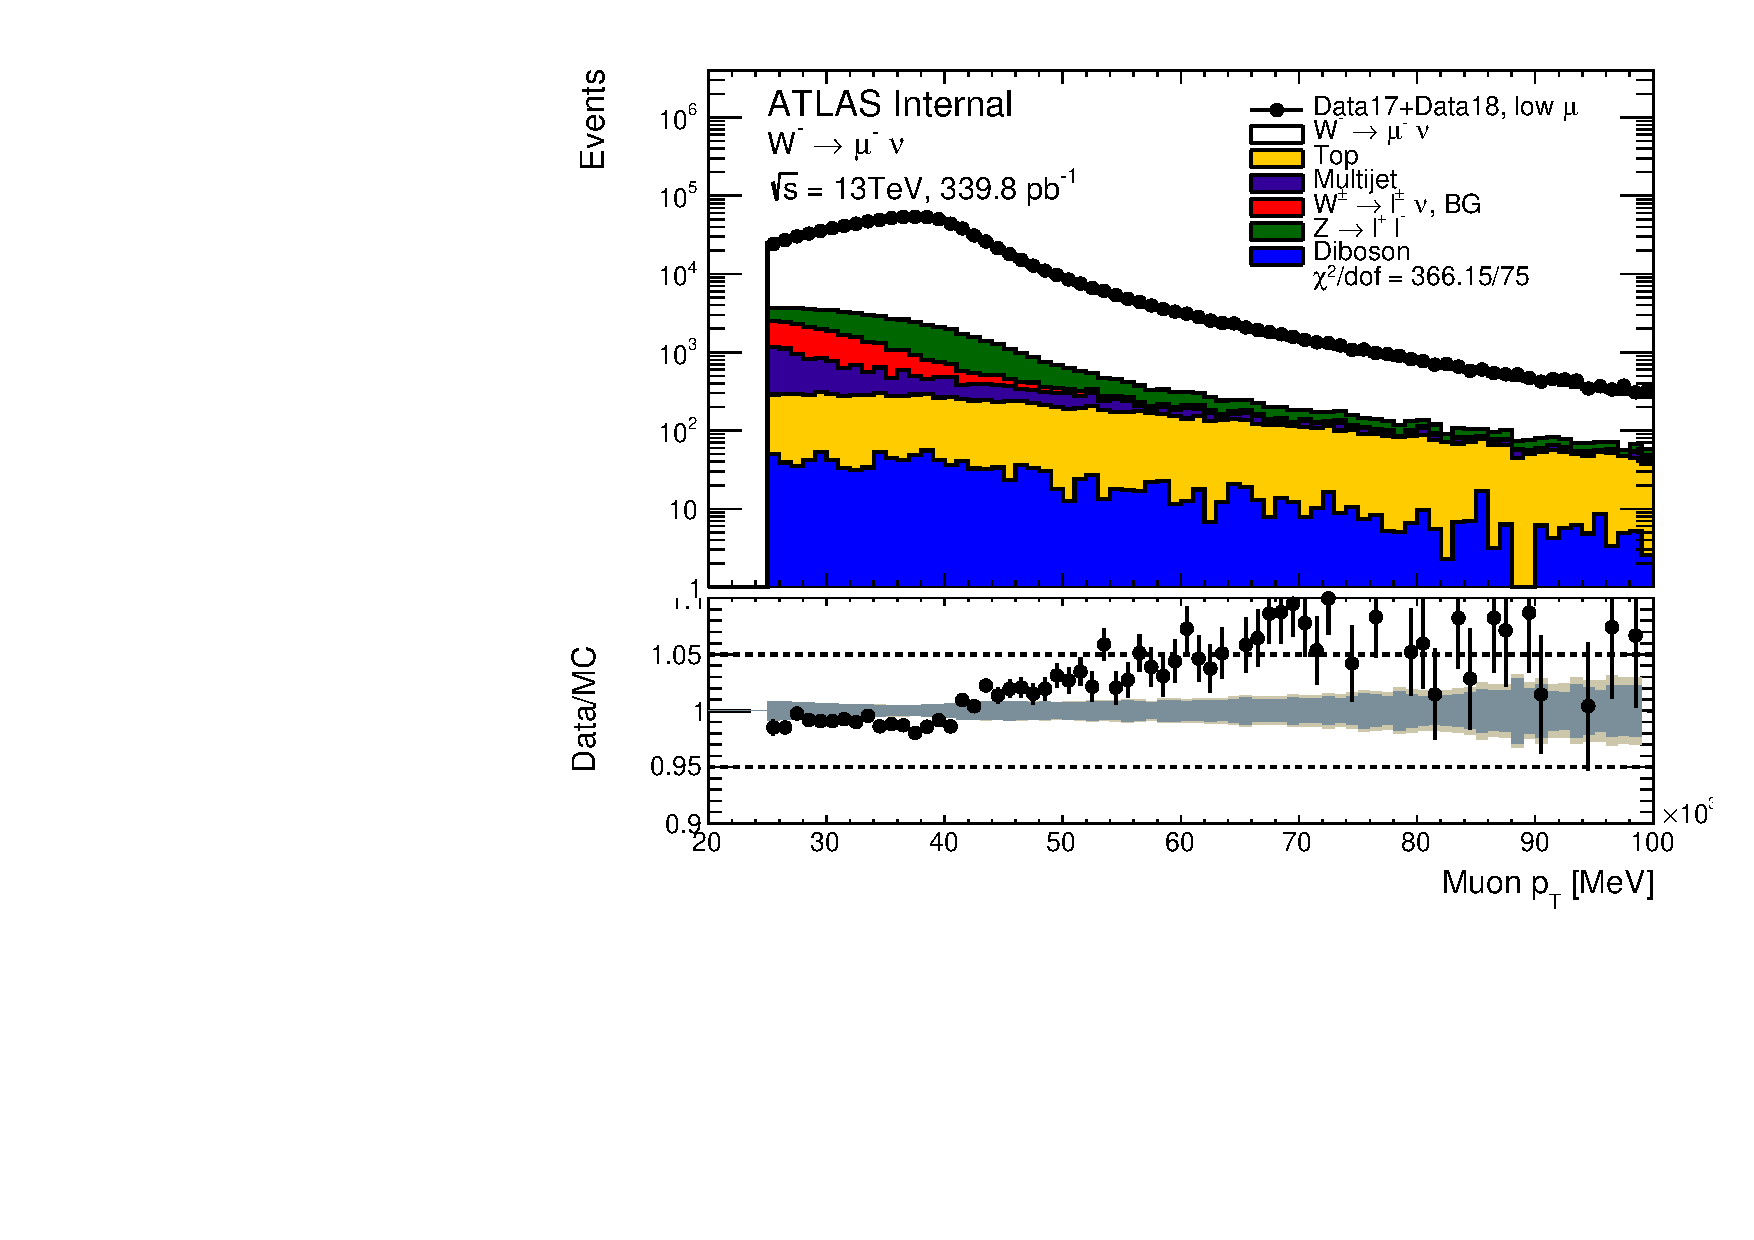
\includegraphics[width=.49\textwidth]{control_norm/muPt_cut7_minusmunu_13TeV_log_norm_NormErr.pdf}\label{f:}}
	{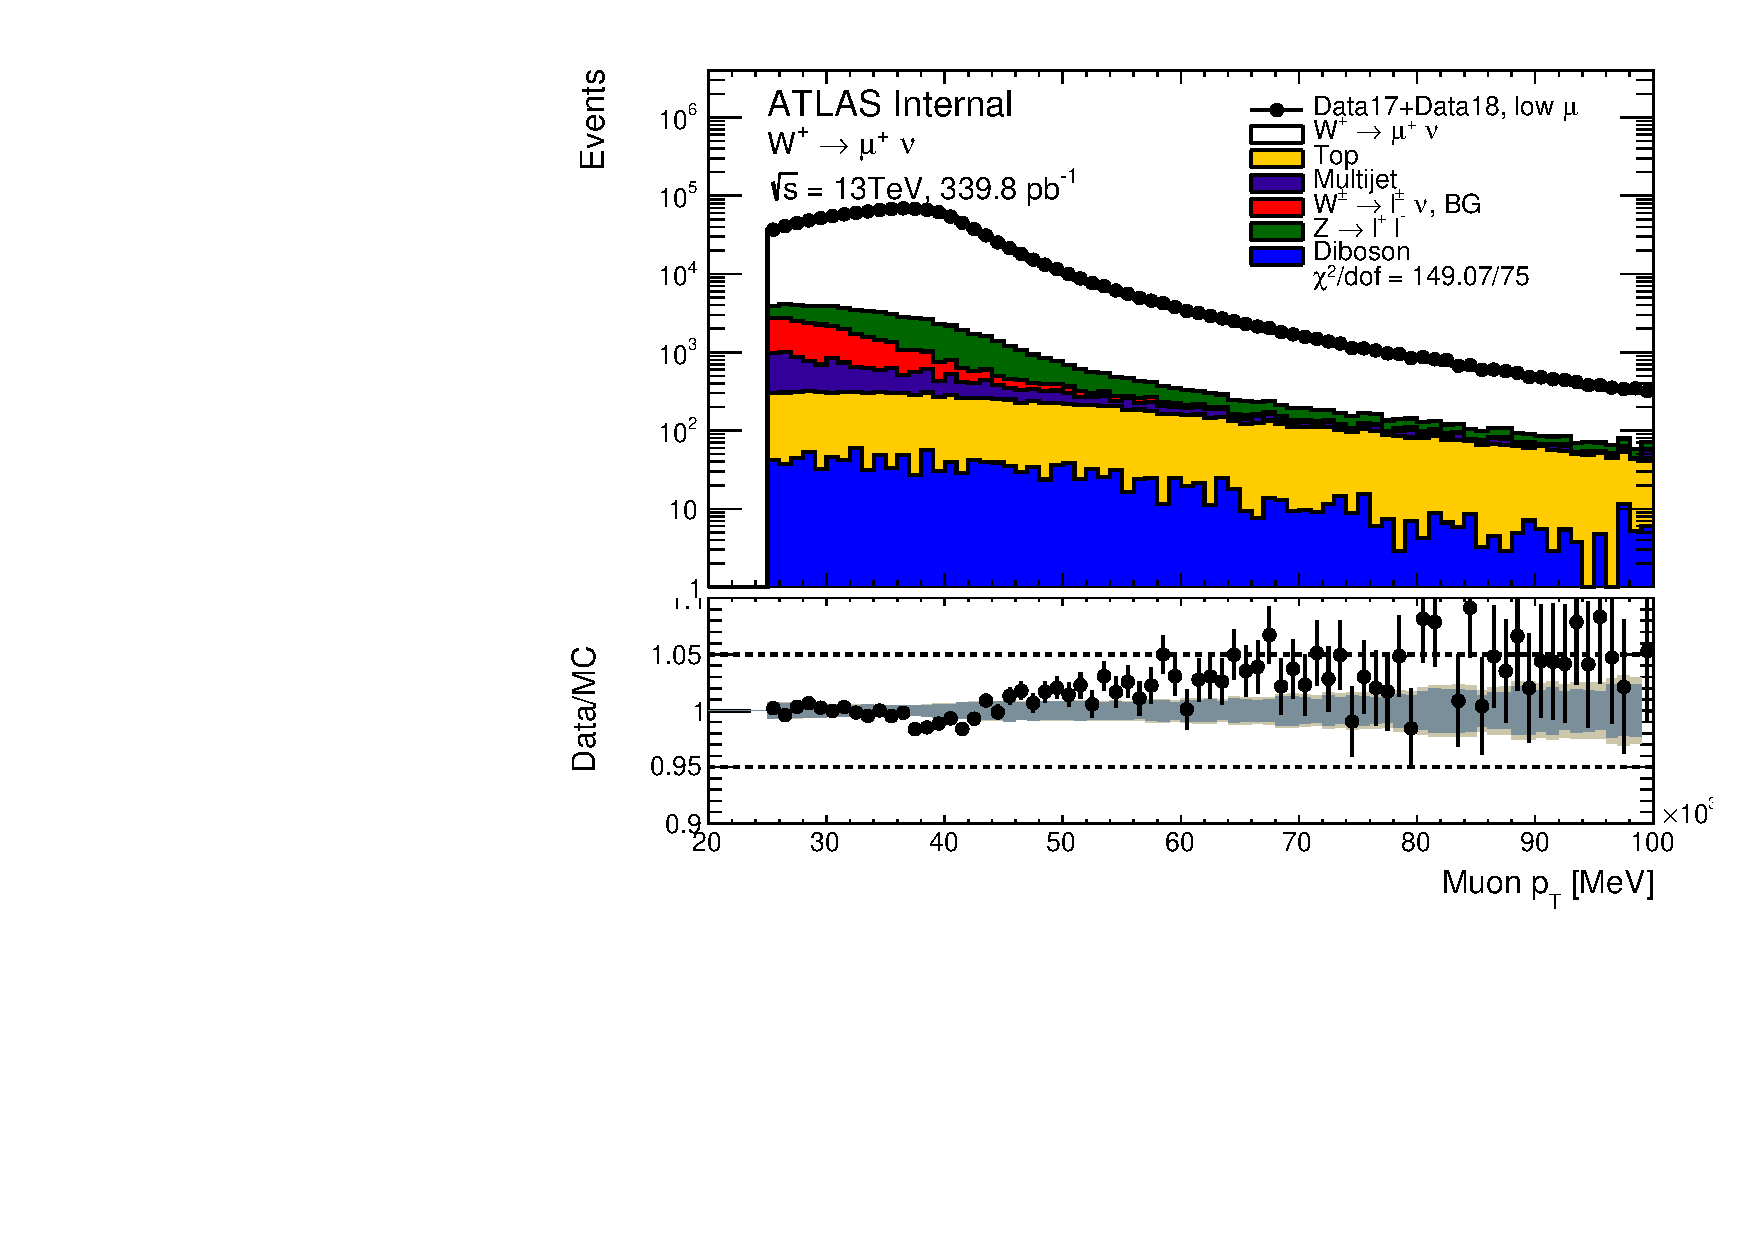
\includegraphics[width=.49\textwidth]{control_norm/muPt_cut7_plusmunu_13TeV_log_norm_NormErr.pdf}\label{f:}}
	
	{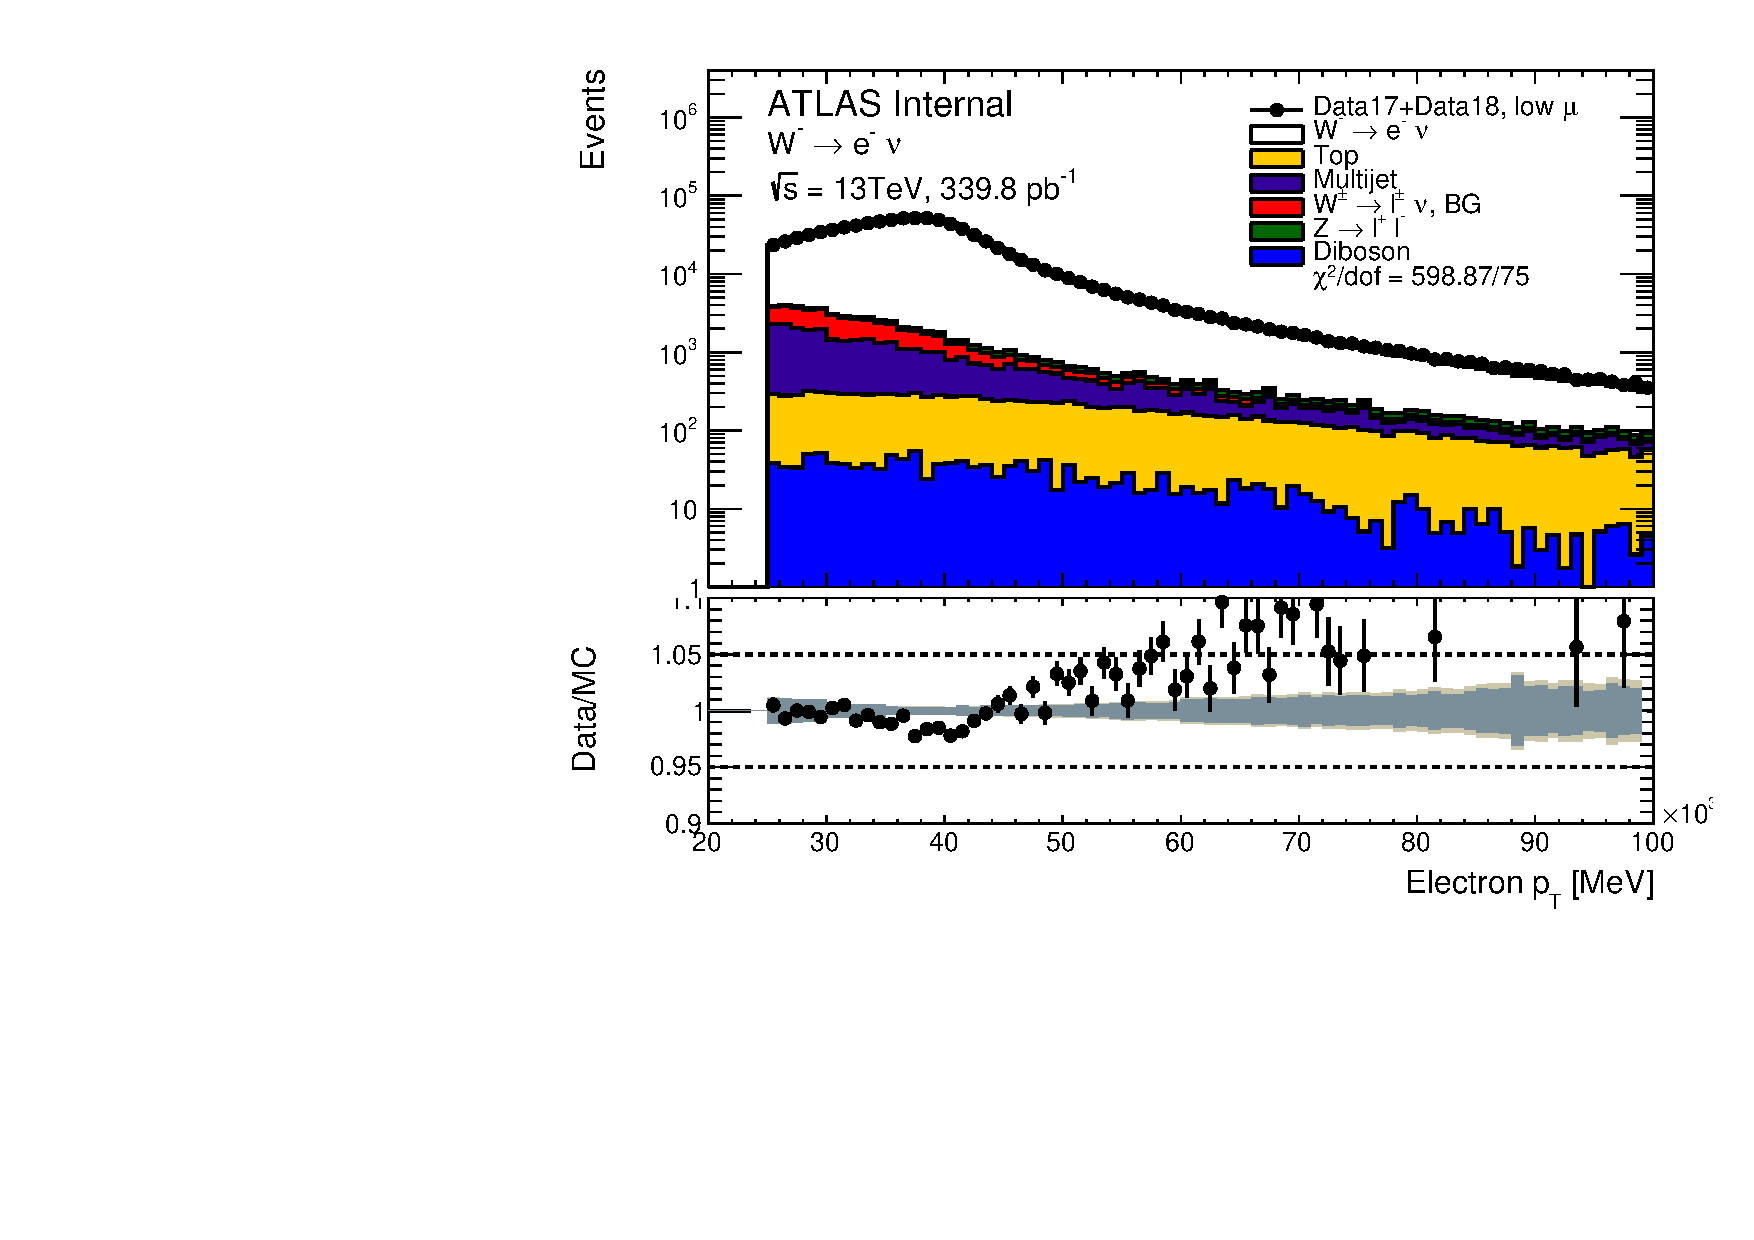
\includegraphics[width=.49\textwidth]{control_norm/elPt_cut7_minusenu_13TeV_log_norm_NormErr.pdf}\label{f:}}
	{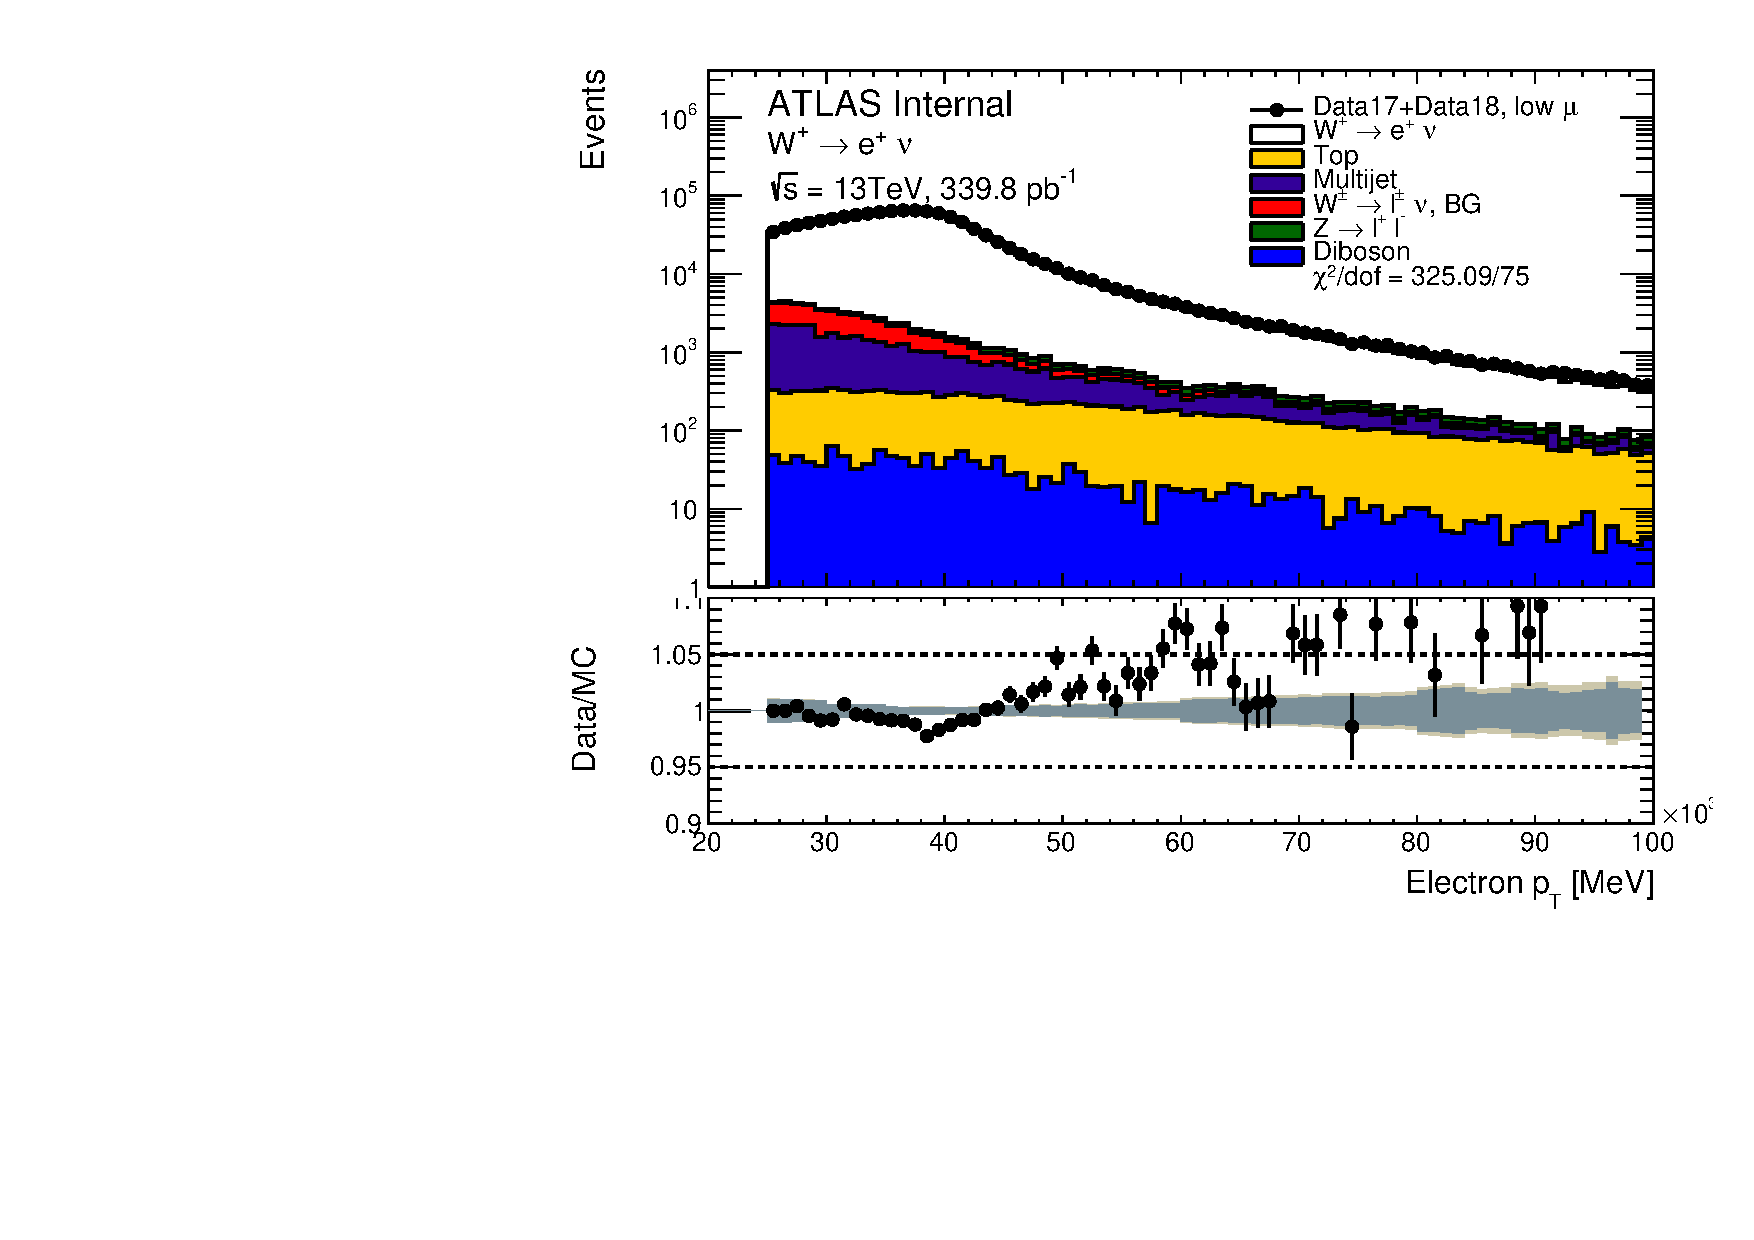
\includegraphics[width=.49\textwidth]{control_norm/elPt_cut7_plusenu_13TeV_log_norm_NormErr.pdf}\label{f:}}
	\caption{  Lepton transverse momentum distribution in the muon and electron channel  for the $\sqrt{s} = 13$~\TeV\ dataset. }\end{figure}



\begin{figure}[h]
	\centering
	{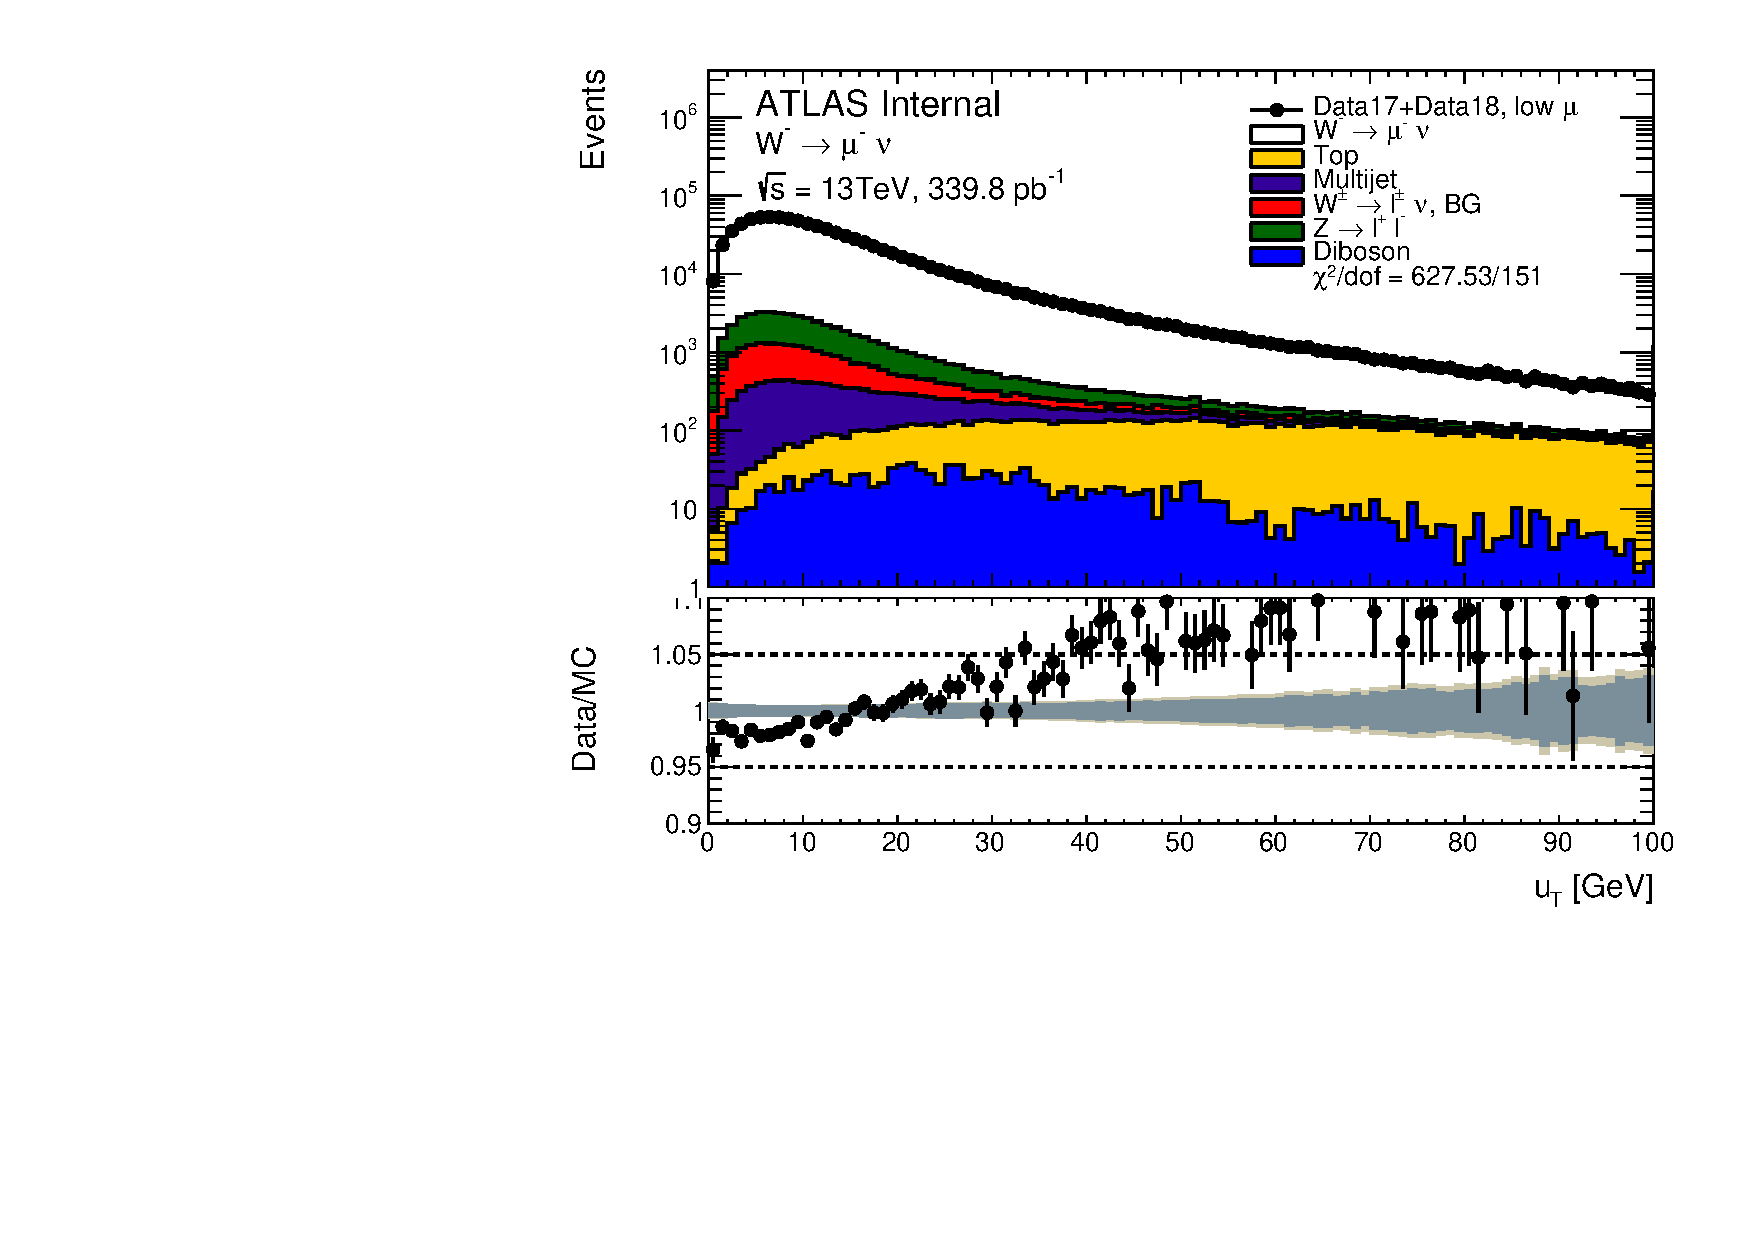
\includegraphics[width=.49\textwidth]{control_norm/WpT_Reco_cut7_minusmunu_13TeV_log_norm_NormErr.pdf}\label{f:}}
	{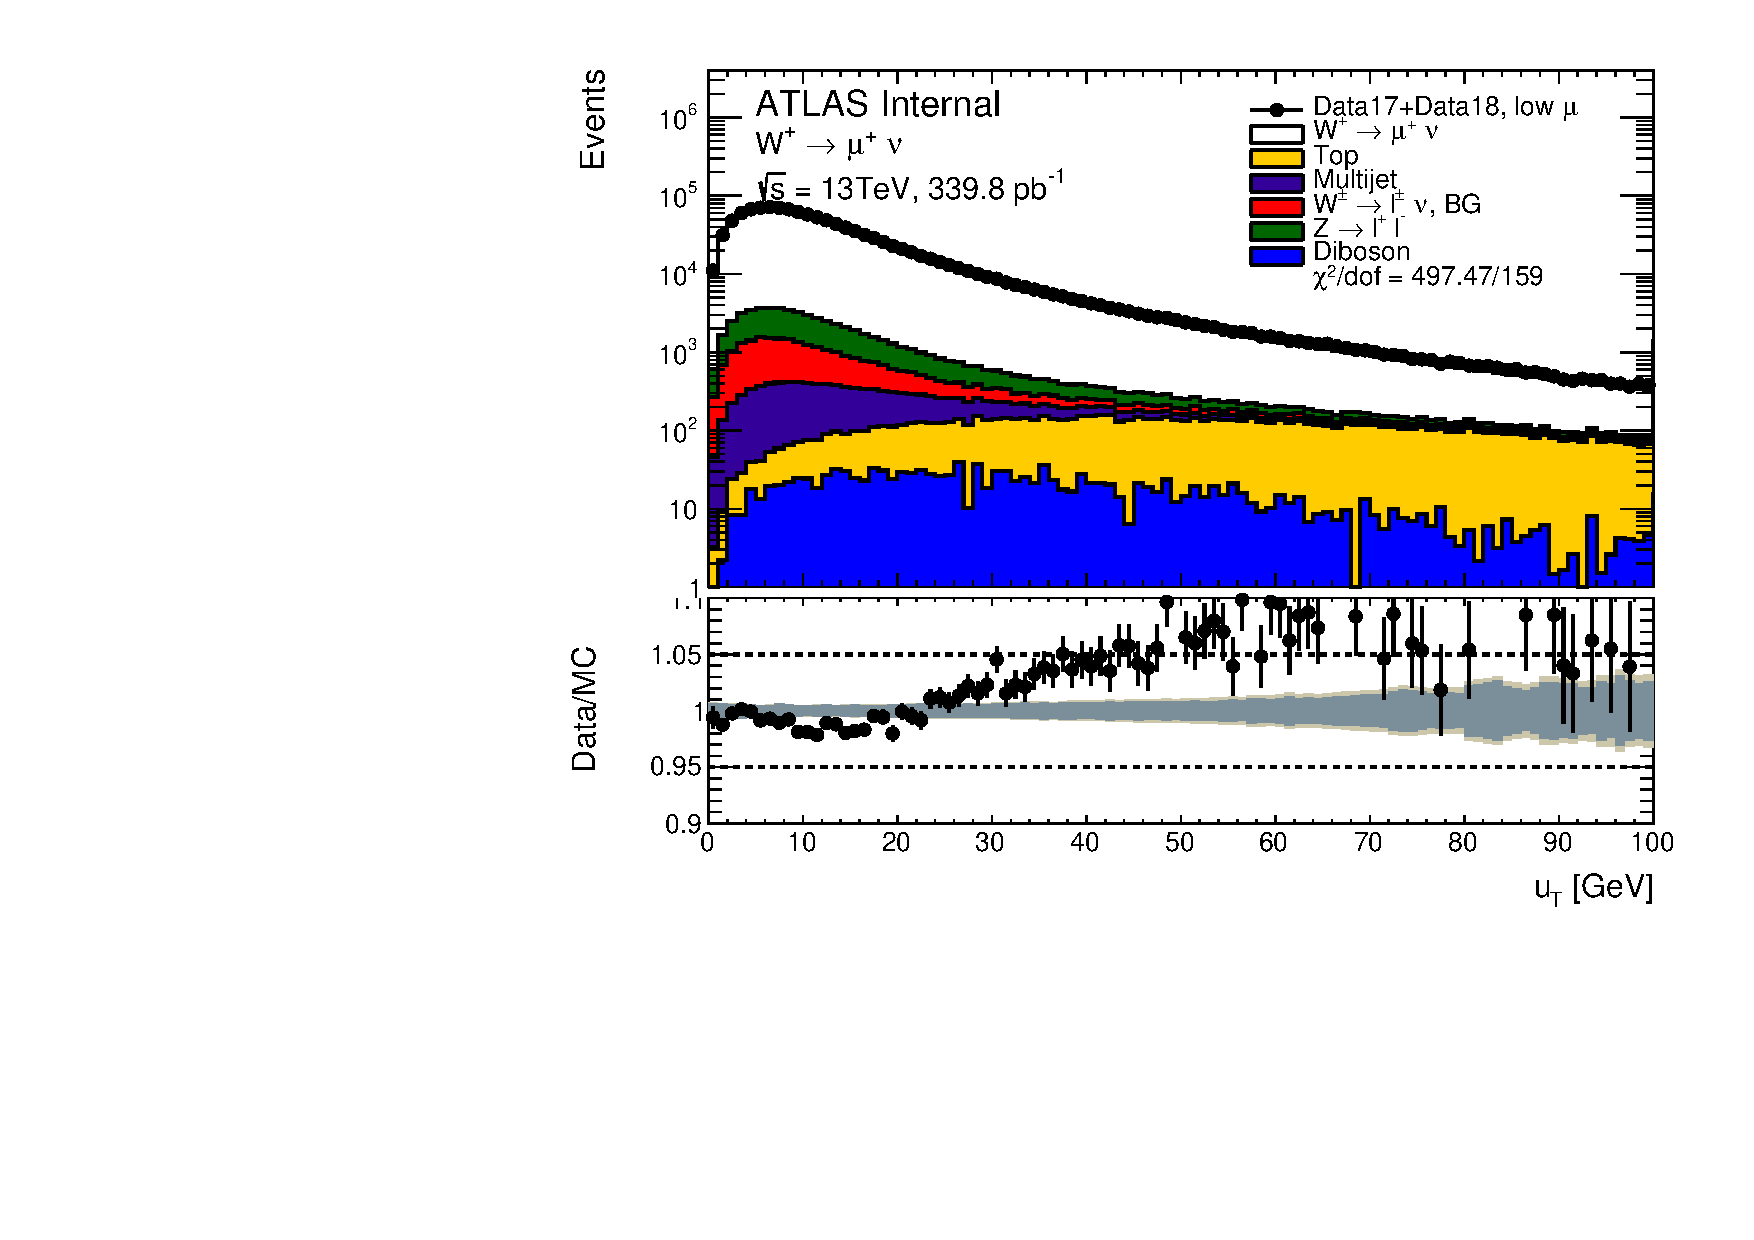
\includegraphics[width=.49\textwidth]{control_norm/WpT_Reco_cut7_plusmunu_13TeV_log_norm_NormErr.pdf}\label{f:}}
	
	{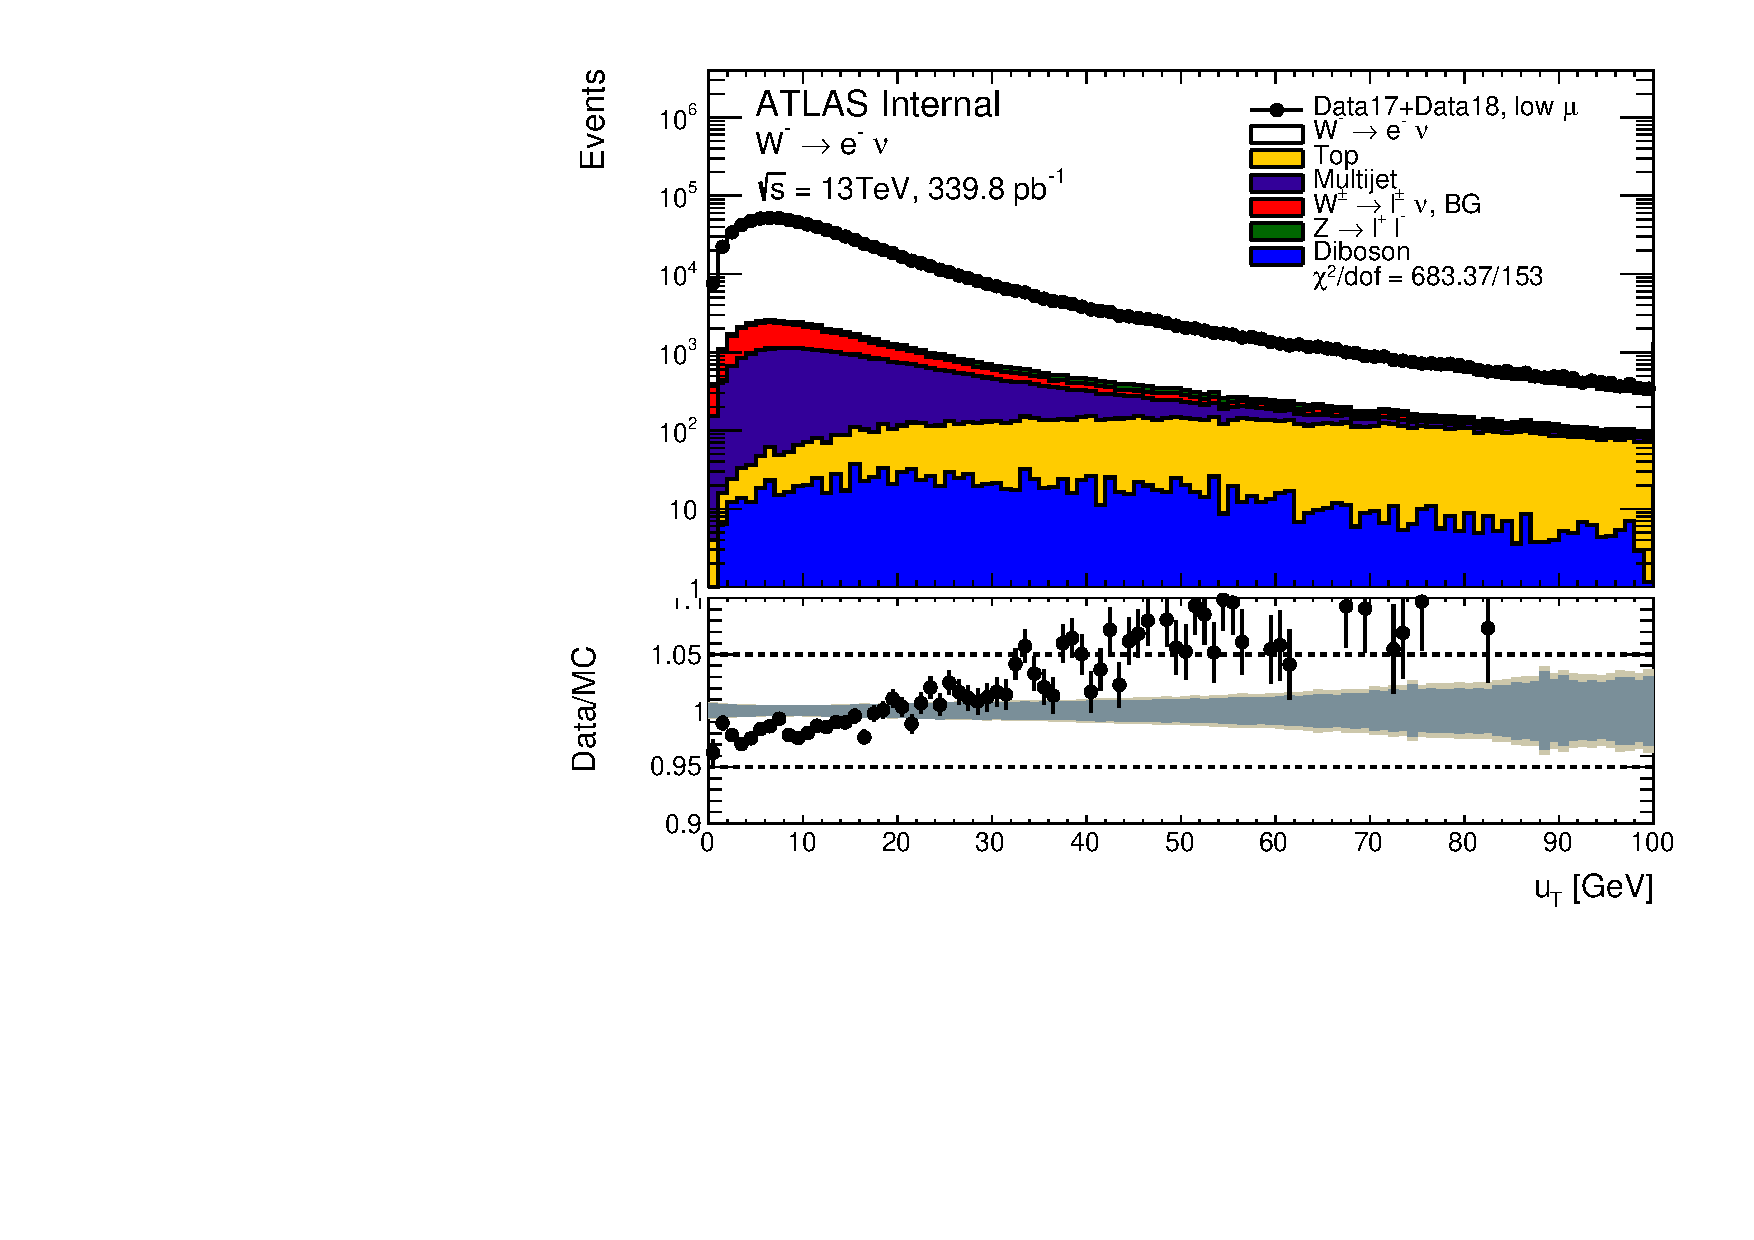
\includegraphics[width=.49\textwidth]{control_norm/WpT_Reco_cut7_minusenu_13TeV_log_norm_NormErr.pdf}\label{f:}}
	{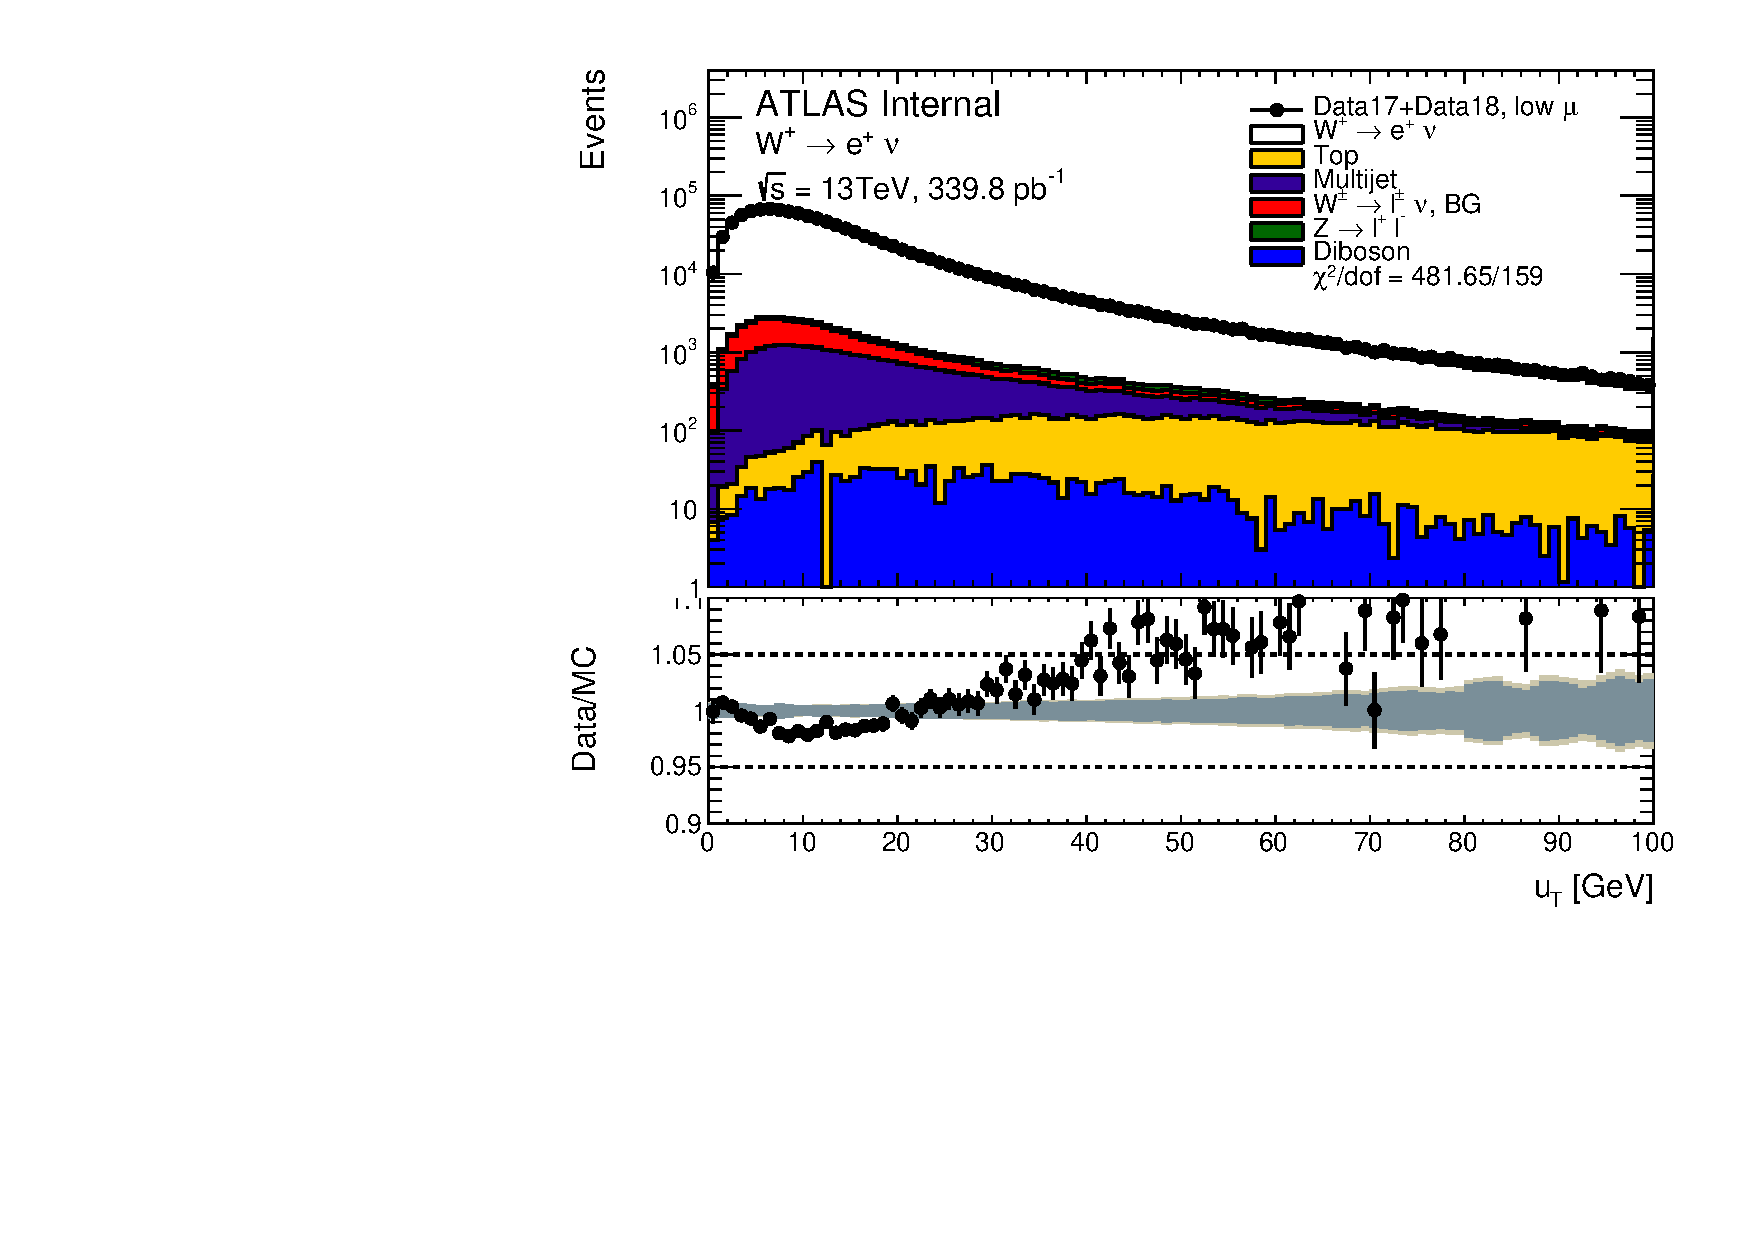
\includegraphics[width=.49\textwidth]{control_norm/WpT_Reco_cut7_plusenu_13TeV_log_norm_NormErr.pdf}\label{f:}}
	\caption{  W transverse momentum distribution in the muon and electron channel  for the $\sqrt{s} = 13$~\TeV\ dataset. }\end{figure}

%%%%% ************************* 5 TeV ****************************

\clearpage


\subsection{$\sqrt{s} = 5$~\TeV\ dataset control plots}
\label{subsec:controlplots5}
Control plots for the 5~\TeV\ \lowmu\ dataset are provided here after applying all corrections described in section~\ref{sec:objects}, and after applying the selection described above in this section. In each figure, the right(left)-hand column shows distributions for the \Wplus\ (\Wminus) process. The top (bottom) row shows the muon (electron) decay channel. In the ratio panels, the grey band is the total systematic uncertainty, whilst the brown band adds the MC statistical uncertainty in quadrature on top of it. In regions of the distributions insensitive to the modelling of \ptw\ there is generally good agreement between data and predictions. The bulk of the \mt\ distribution is a typical example of distribution that is mostly insensitive to the modeling of \ptw. Compared to the 13~\TeV\ situation, the \ut\ distribution seems to indicate that the baseline simulation models \ptw\ more satisfactorily.

\begin{figure}[h]
	\centering
	{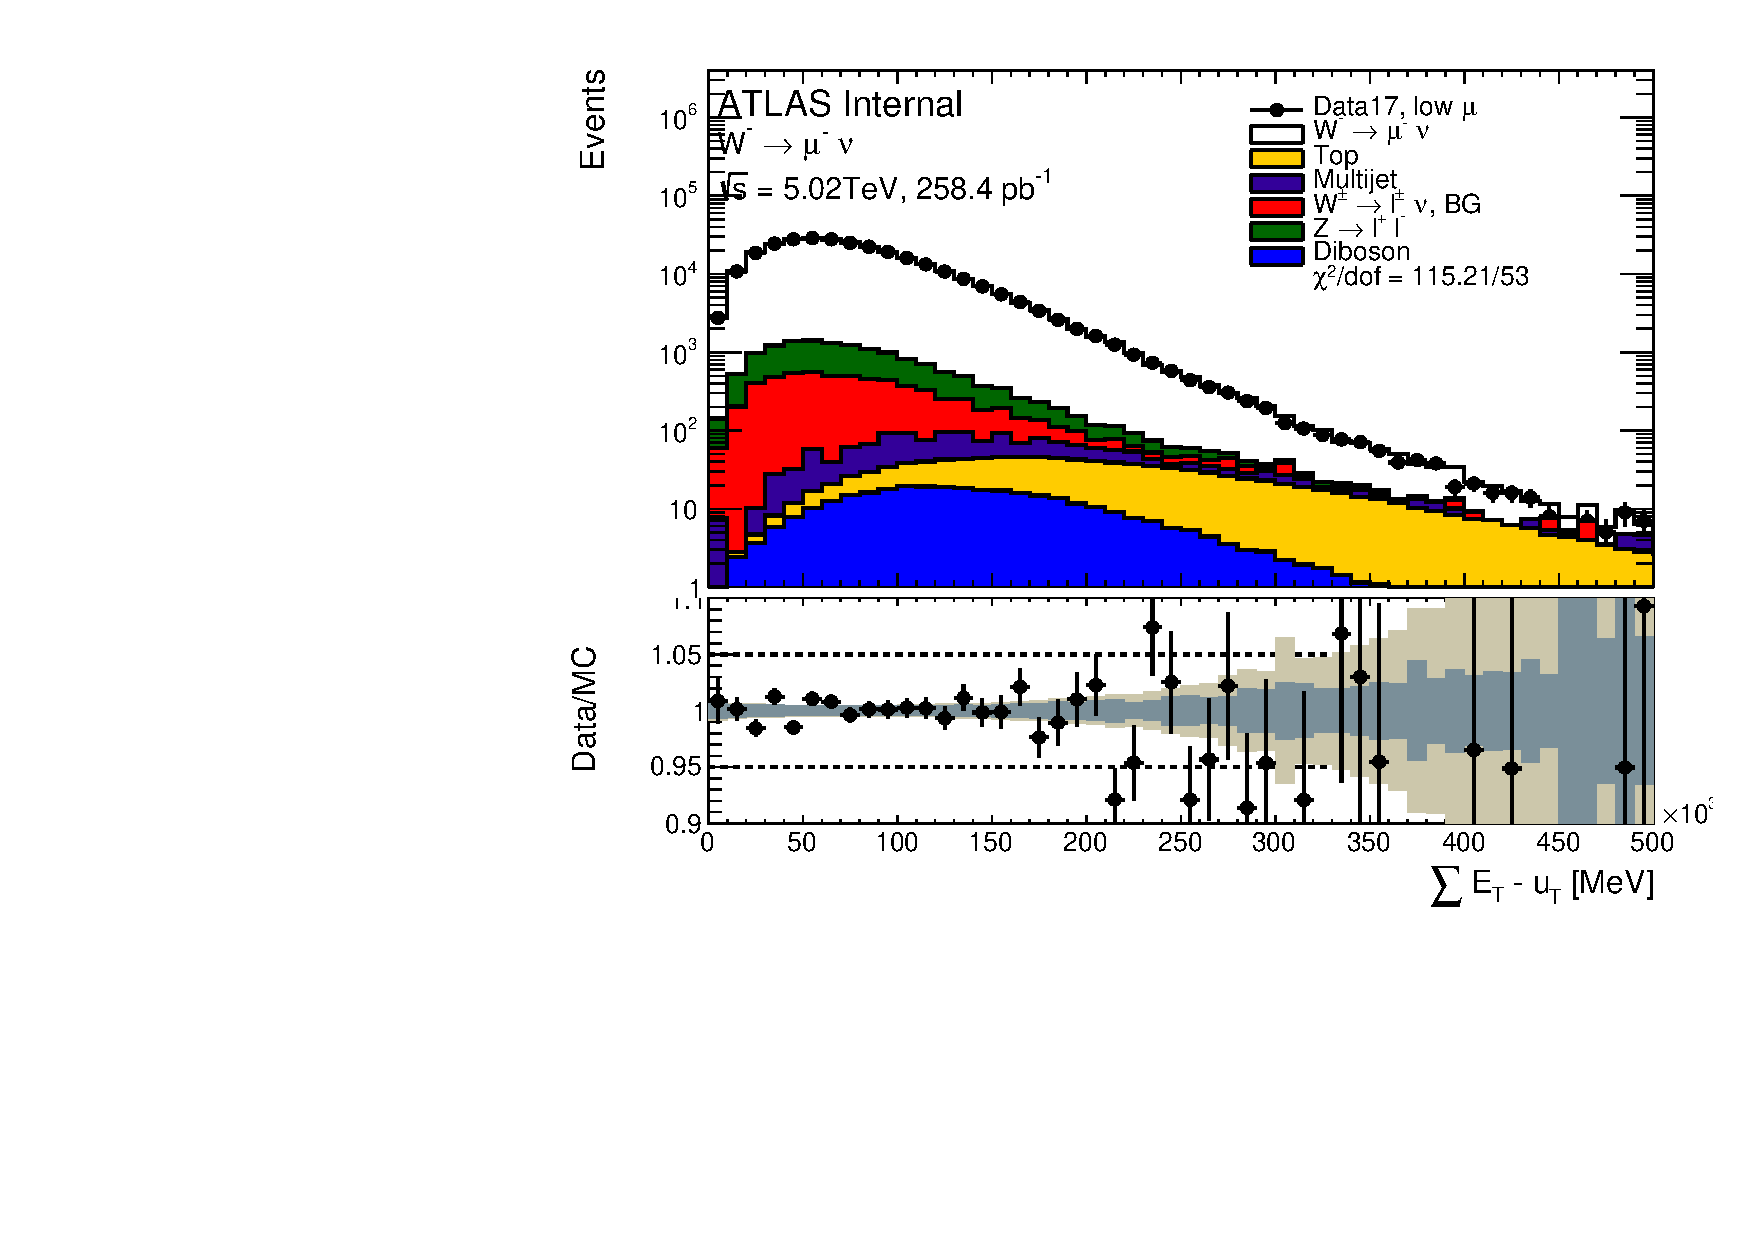
\includegraphics[width=.49\textwidth]{control_norm/SETUE_cut7_minusmunu_5TeV_log_norm_NormErr.pdf}\label{f:SETUEmm5}}
	{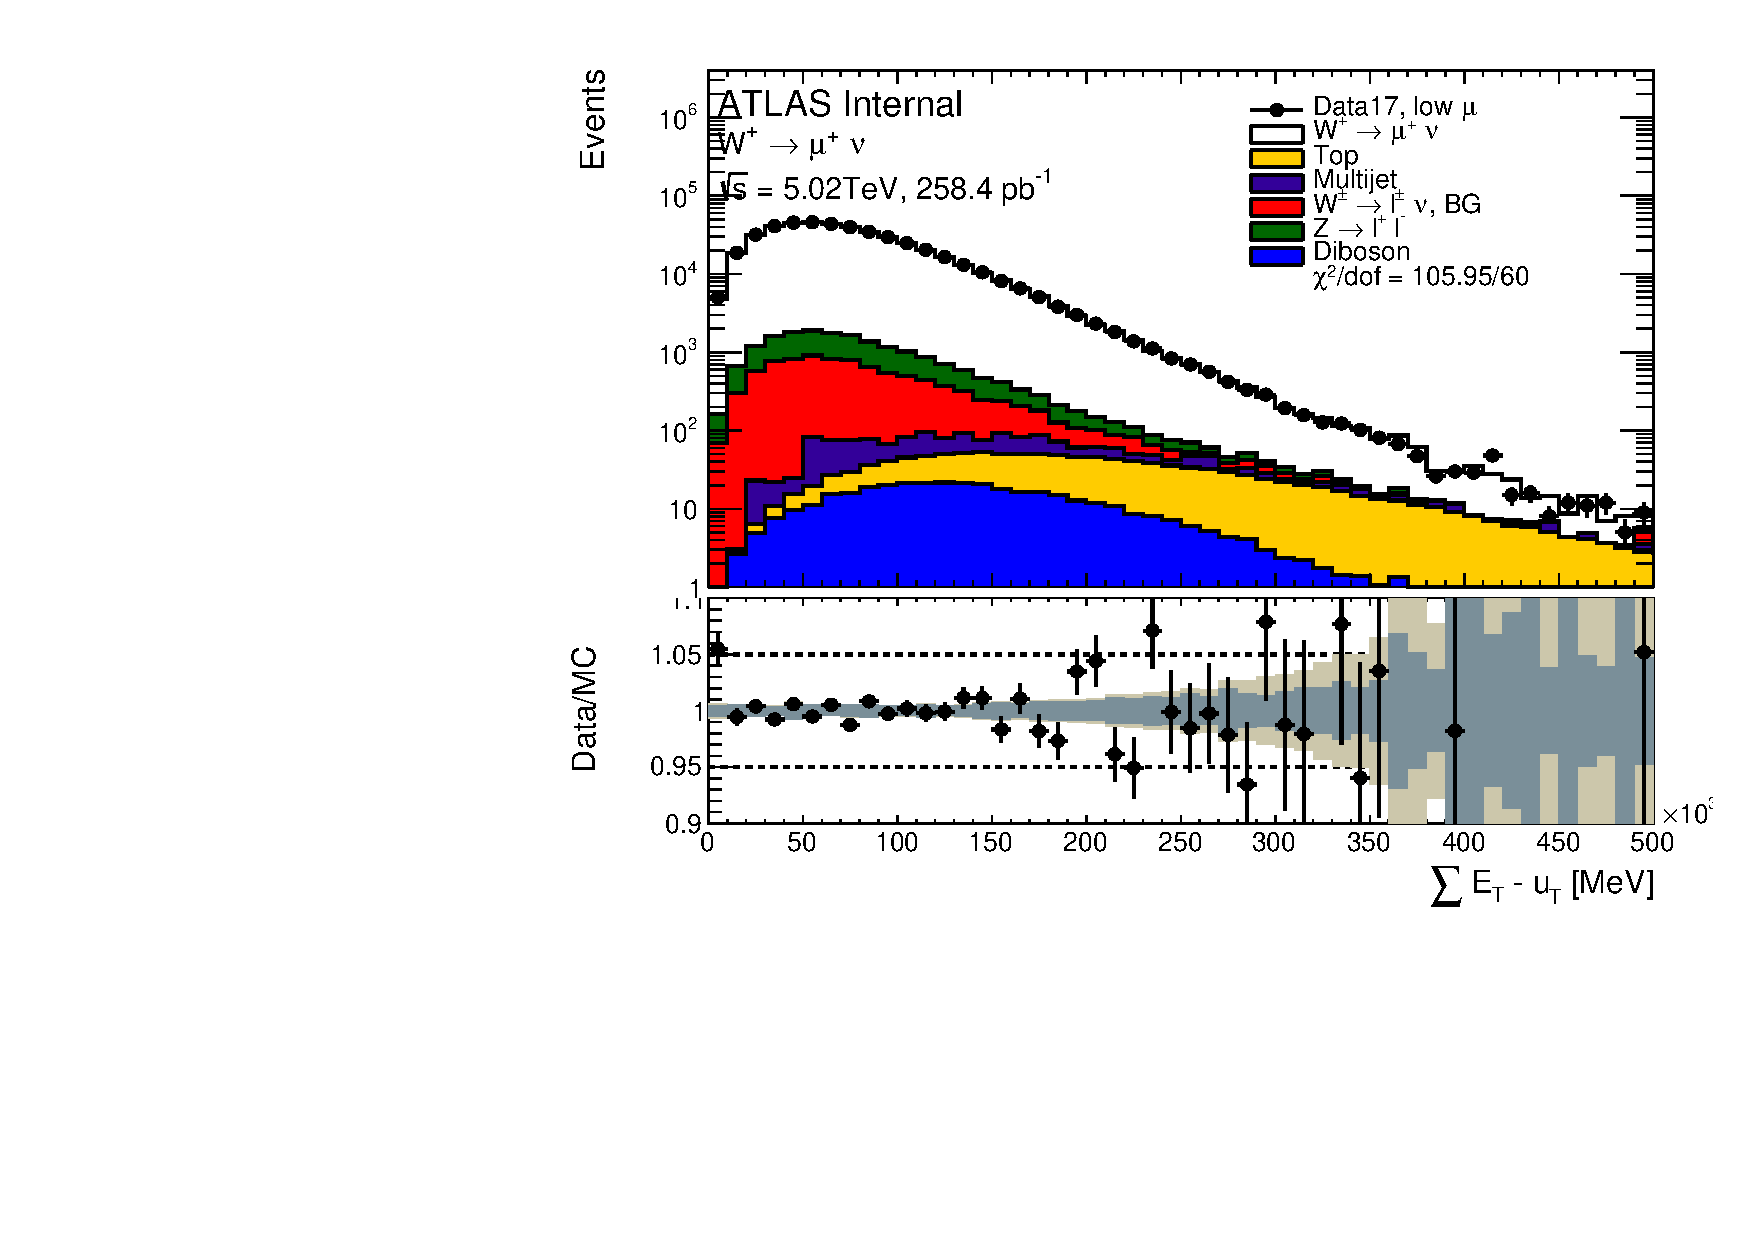
\includegraphics[width=.49\textwidth]{control_norm/SETUE_cut7_plusmunu_5TeV_log_norm_NormErr.pdf}\label{f:SETUEpm5}}
	
	{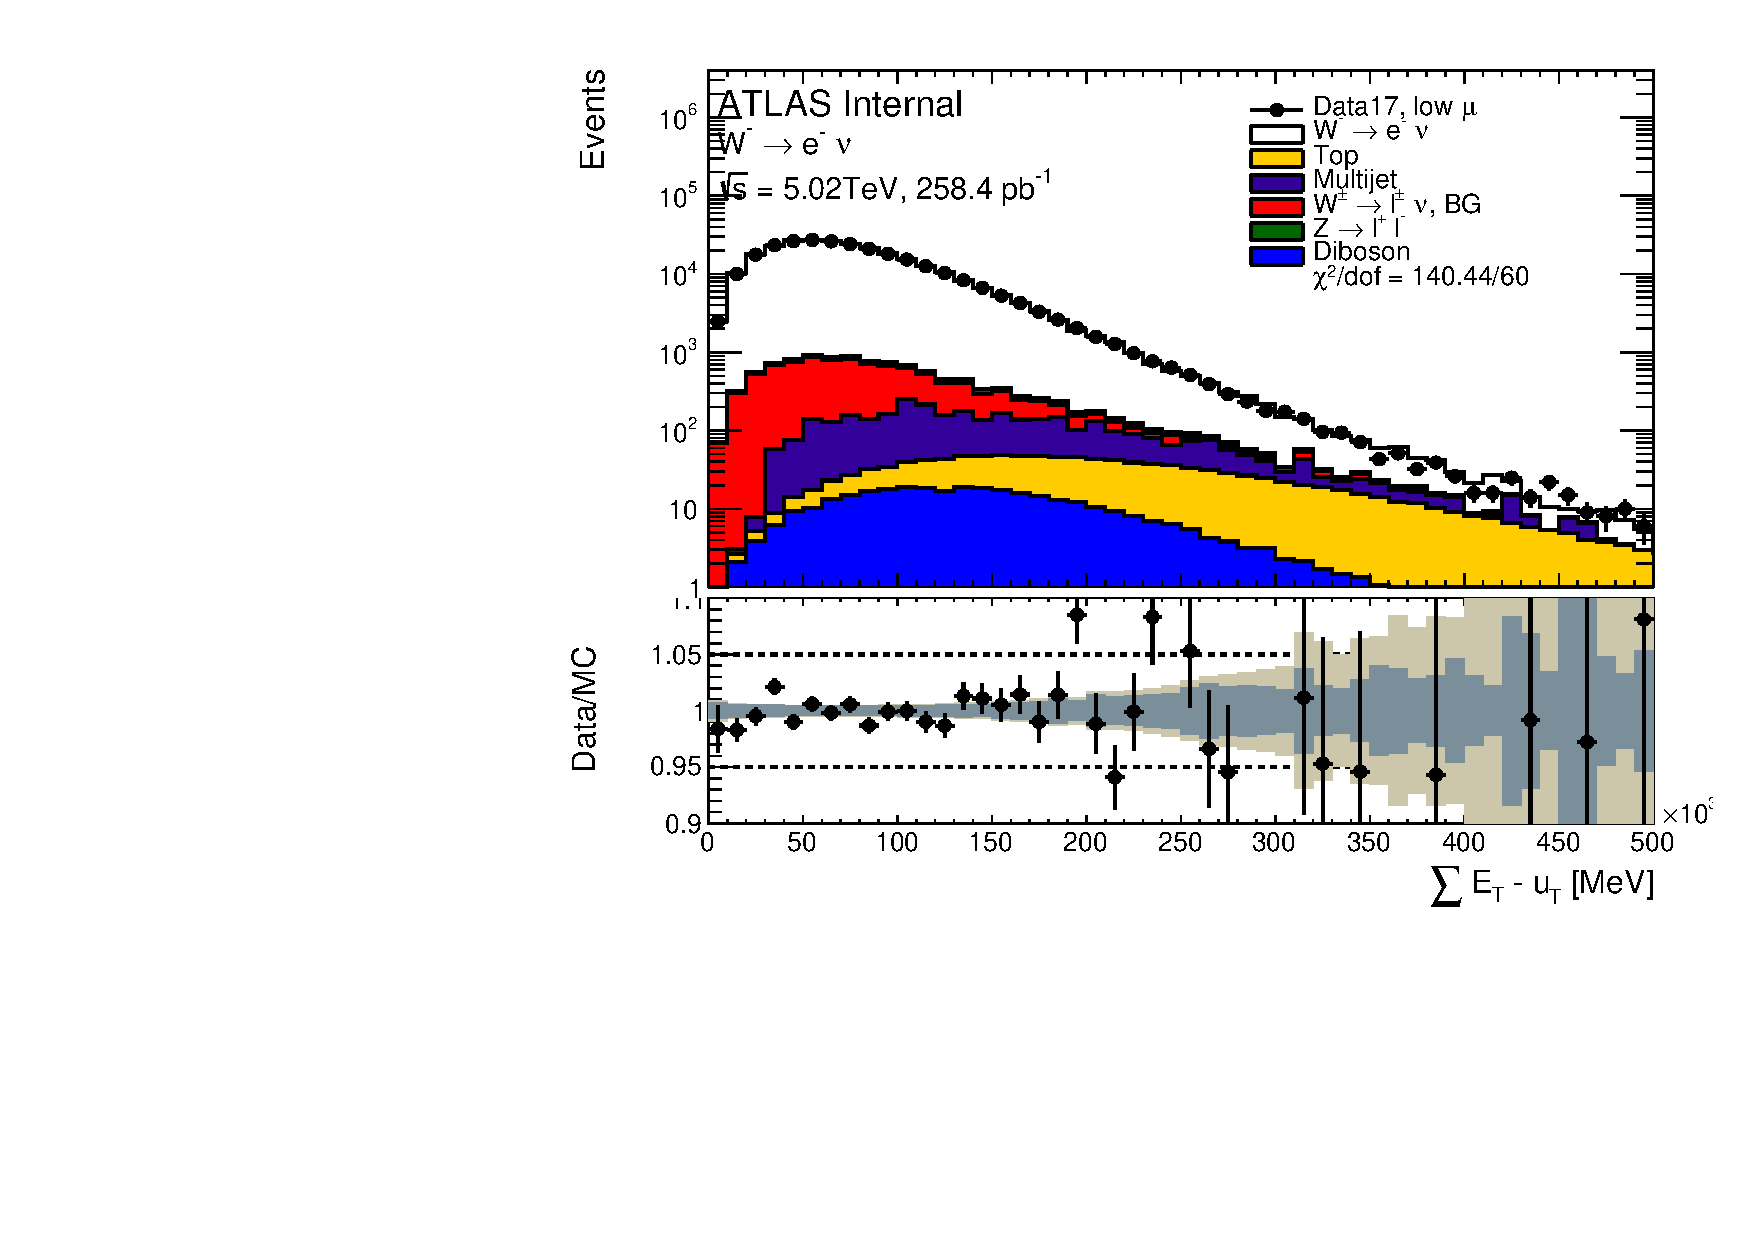
\includegraphics[width=.49\textwidth]{control_norm/SETUE_cut7_minusenu_5TeV_log_norm_NormErr.pdf}\label{f:}}
	{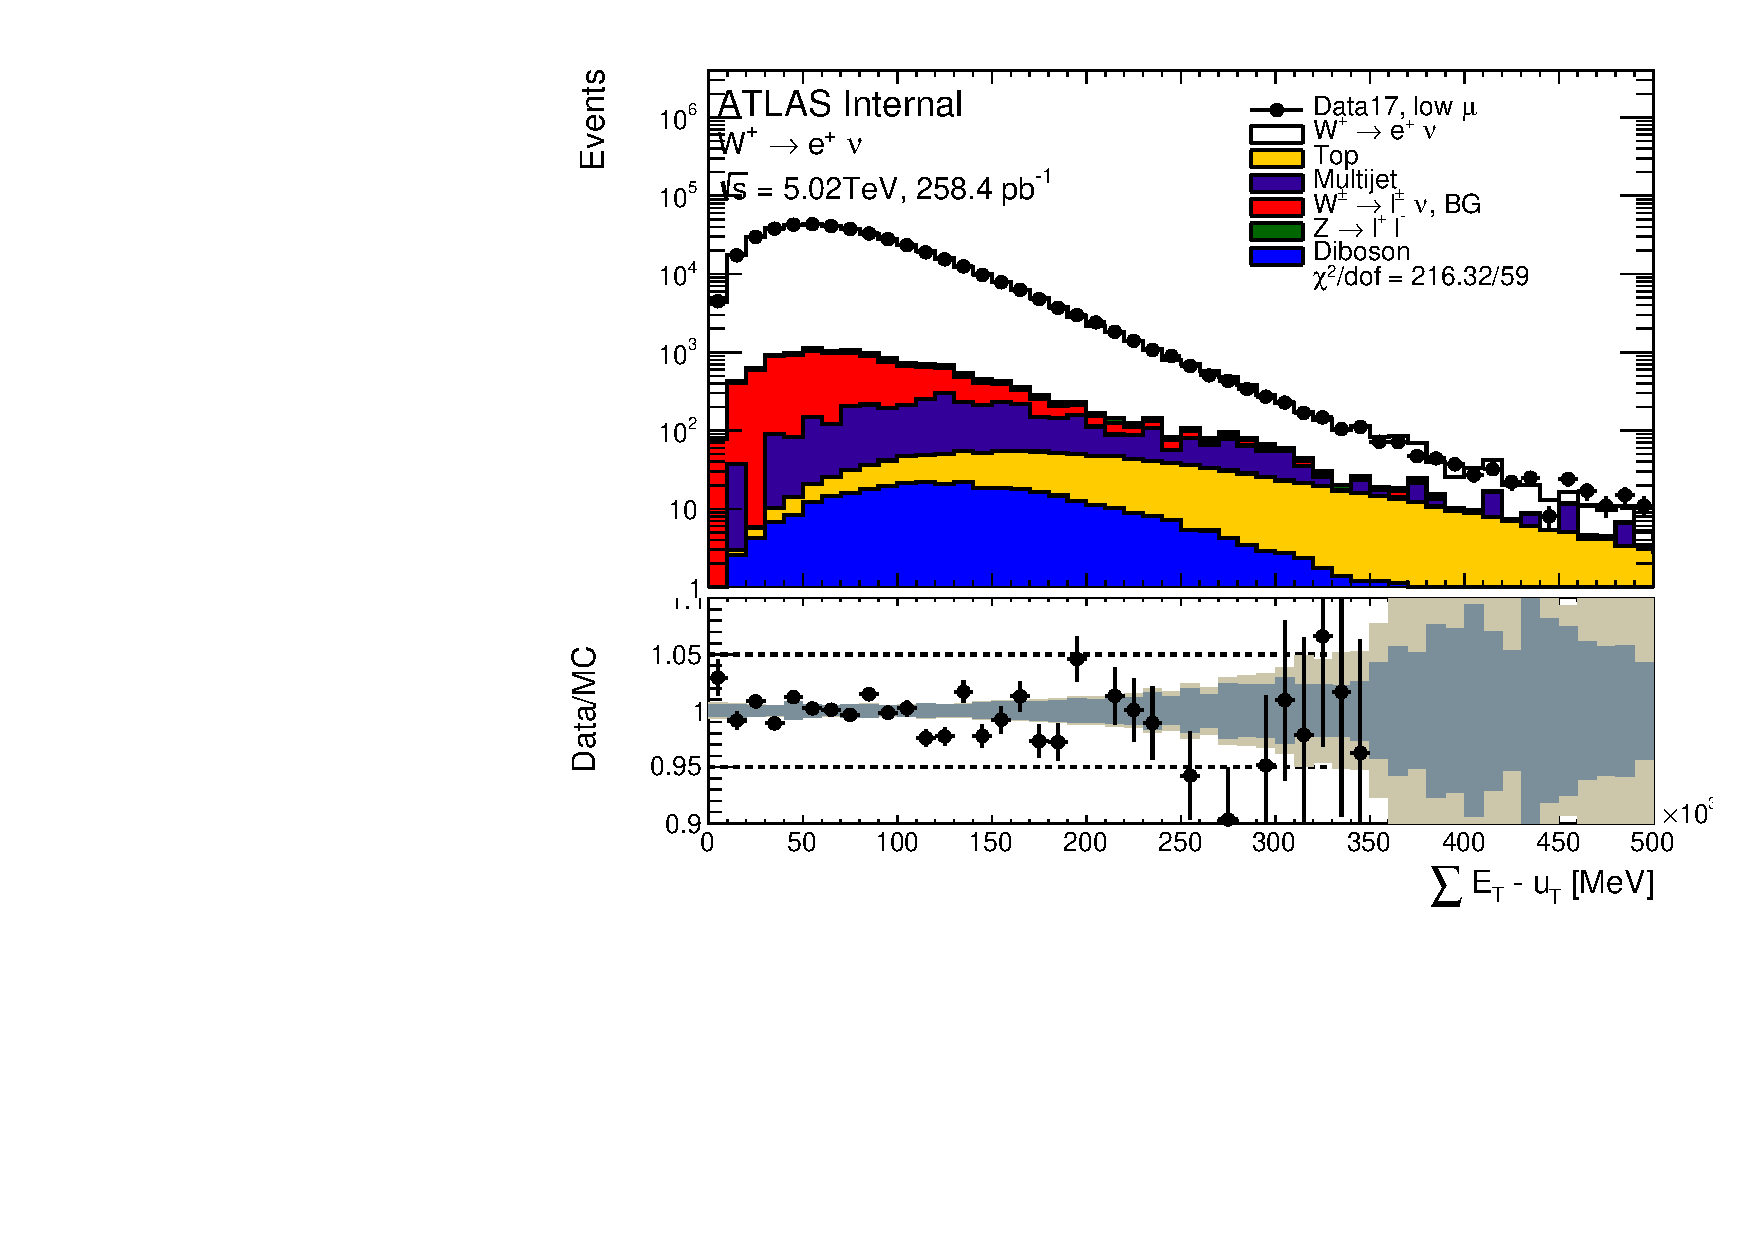
\includegraphics[width=.49\textwidth]{control_norm/SETUE_cut7_plusenu_5TeV_log_norm_NormErr.pdf}\label{f:}}
	\caption{$\Sigma \bar{E_T}$ distribution in the muon and electron channel  for the $\sqrt{s} = 5$~\TeV\ dataset.}
\end{figure}
%

\begin{figure}[h]
	\centering
	{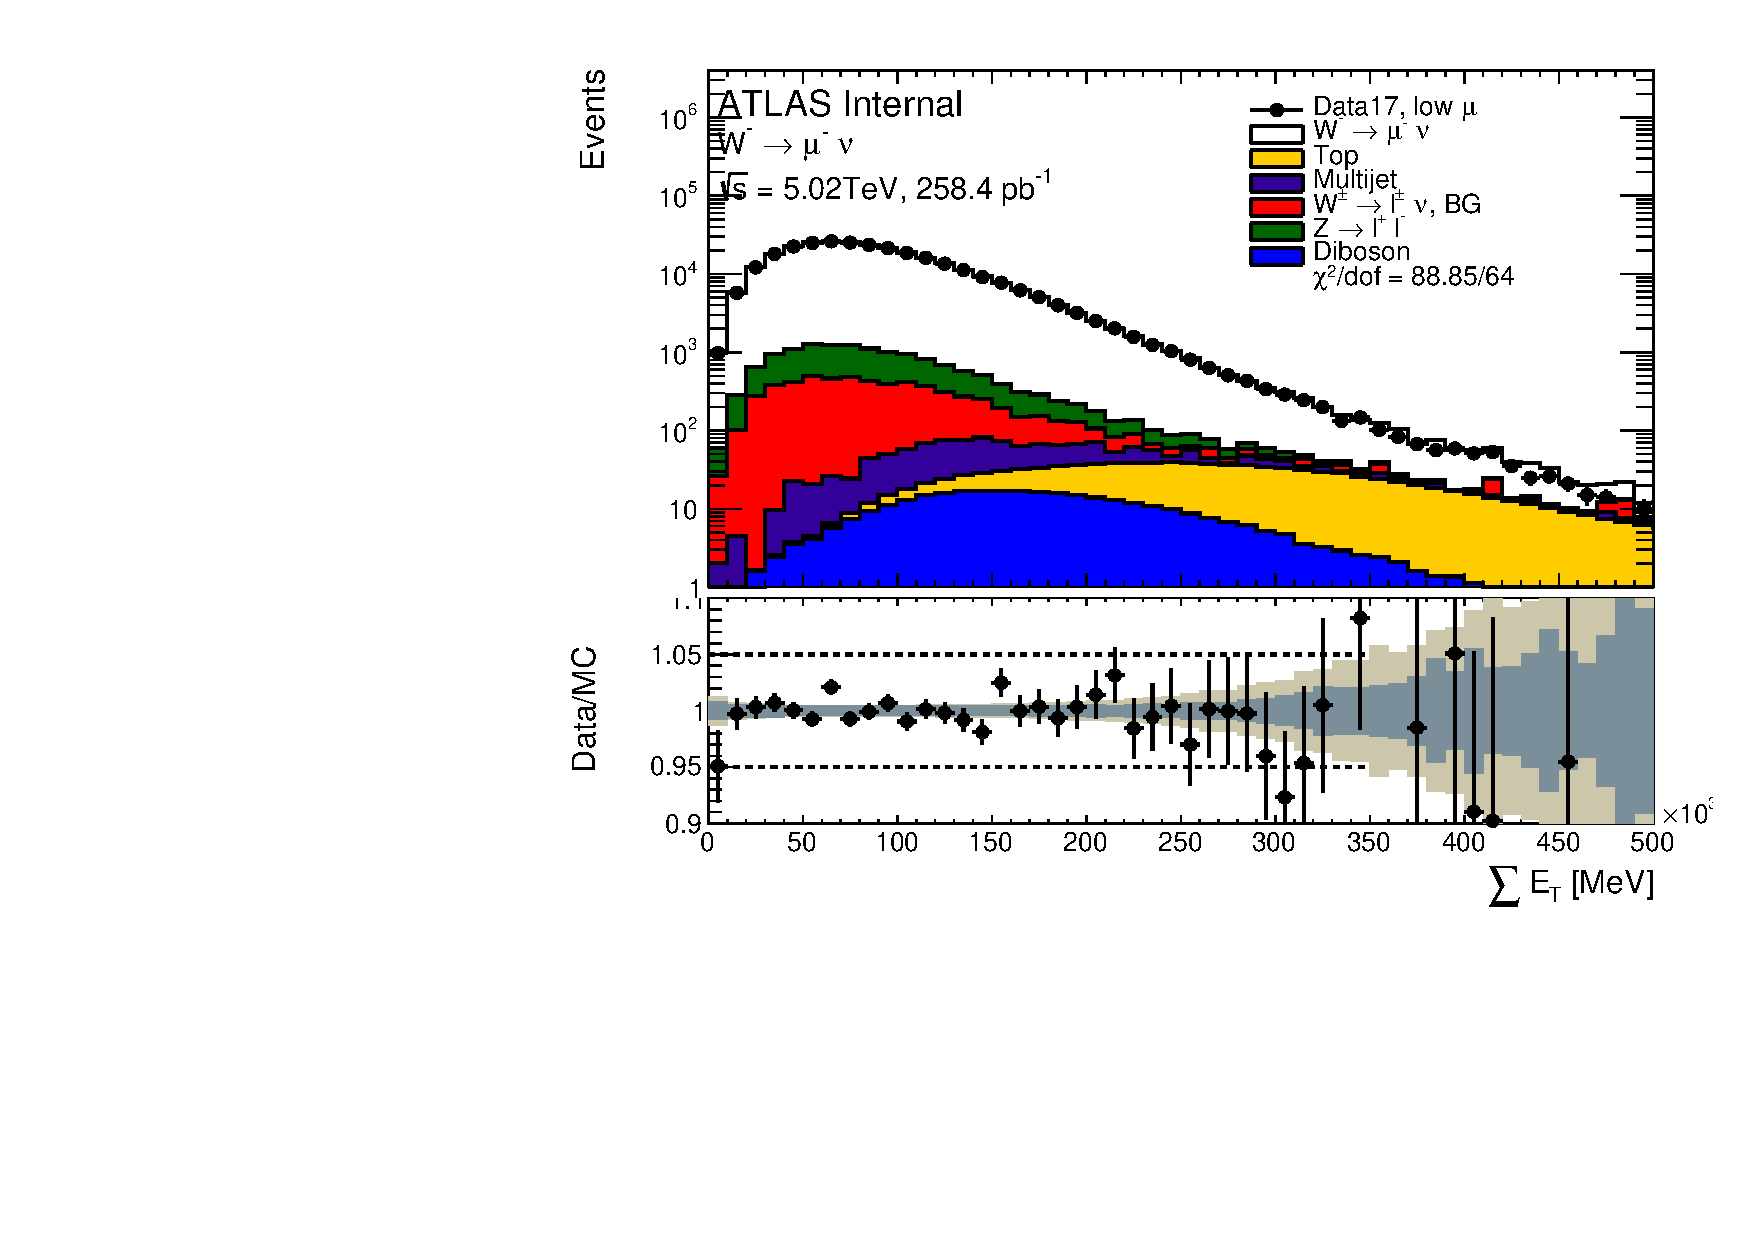
\includegraphics[width=.49\textwidth]{control_norm/SET_cut7_minusmunu_5TeV_log_norm_NormErr.pdf}\label{f:set5}}
	{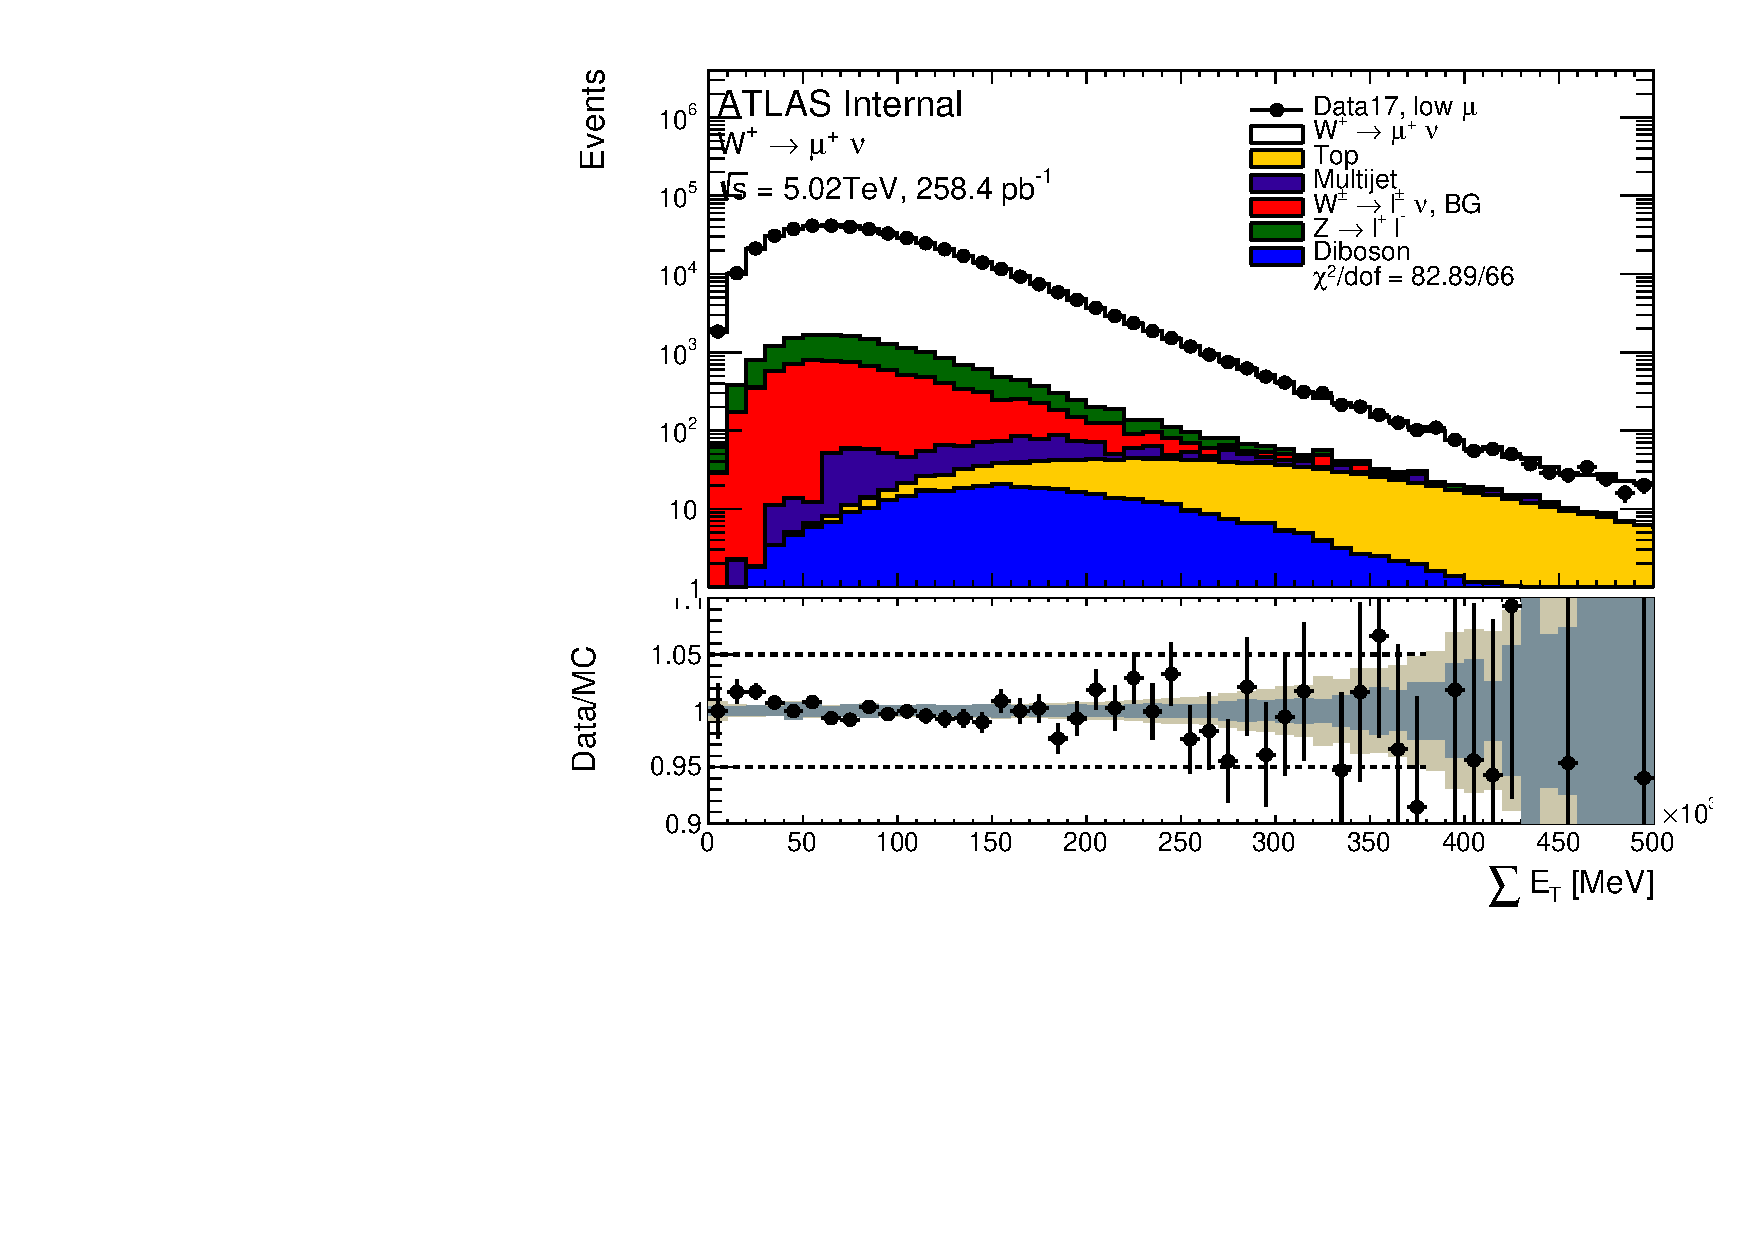
\includegraphics[width=.49\textwidth]{control_norm/SET_cut7_plusmunu_5TeV_log_norm_NormErr.pdf}\label{f:setpl}}
	
	{\includegraphics[width=.49\textwidth]{control_norm/SET_cut7_minusenu_5TeV_log_norm_NormErr.pdf}\label{f:}}
	{\includegraphics[width=.49\textwidth]{control_norm/SET_cut7_plusenu_5TeV_log_norm_NormErr.pdf}\label{f:}}
	\caption{$\Sigma{E_T}$ distribution in the muon and electron channel  for the $\sqrt{s} = 5$~\TeV\ dataset.}
\end{figure}
\newpage


\begin{figure}[h]
	\centering
	{\includegraphics[width=.49\textwidth]{control_norm/met_cut7_minusmunu_5TeV_log_norm_NormErr.pdf}\label{f:}}
	{\includegraphics[width=.49\textwidth]{control_norm/met_cut7_plusmunu_5TeV_log_norm_NormErr.pdf}\label{f:}}
	
	{\includegraphics[width=.49\textwidth]{control_norm/met_cut7_minusenu_5TeV_log_norm_NormErr.pdf}\label{f:}}
	{\includegraphics[width=.49\textwidth]{control_norm/met_cut7_plusenu_5TeV_log_norm_NormErr.pdf}\label{f:}}
	\caption{ $\vec{E}^{miss}_{T}$ distribution in the muon and electron channel  for the $\sqrt{s} = 5$~\TeV\ dataset.}
\end{figure}
\newpage



\begin{figure}[h]
	\centering
	{\includegraphics[width=.49\textwidth]{control_norm/mT_cut7_minusmunu_5TeV_log_norm_NormErr.pdf}\label{f:}}
	{\includegraphics[width=.49\textwidth]{control_norm/mT_cut7_plusmunu_5TeV_log_norm_NormErr.pdf}\label{f:}}
	
	{\includegraphics[width=.49\textwidth]{control_norm/mT_cut7_minusenu_5TeV_log_norm_NormErr.pdf}\label{f:}}
	{\includegraphics[width=.49\textwidth]{control_norm/mT_cut7_plusenu_5TeV_log_norm_NormErr.pdf}\label{f:}}
	\caption{  Transverse mass distribution of the W boson in the muon and electron channel  for the $\sqrt{s} = 5$~\TeV\ dataset. }\end{figure}
\newpage

\begin{figure}[h]
	\centering
	{\includegraphics[width=.49\textwidth]{control_norm/muEta_cut7_minusmunu_5TeV_log_norm_NormErr.pdf}\label{f:}}
	{\includegraphics[width=.49\textwidth]{control_norm/muEta_cut7_plusmunu_5TeV_log_norm_NormErr.pdf}\label{f:}}
	
	{\includegraphics[width=.49\textwidth]{control_norm/elEta_cut7_minusenu_5TeV_log_norm_NormErr.pdf}\label{f:}}
	{\includegraphics[width=.49\textwidth]{control_norm/elEta_cut7_plusenu_5TeV_log_norm_NormErr.pdf}\label{f:}}
	\caption{  Lepton pseudorapidity distribution in the muon and electron channel  for the $\sqrt{s} = 5$~\TeV\ dataset. }\end{figure}
\newpage

\begin{figure}[h]
	\centering
	{\includegraphics[width=.49\textwidth]{control_norm/muPt_cut7_minusmunu_5TeV_log_norm_NormErr.pdf}\label{f:}}
	{\includegraphics[width=.49\textwidth]{control_norm/muPt_cut7_plusmunu_5TeV_log_norm_NormErr.pdf}\label{f:}}
	
	{\includegraphics[width=.49\textwidth]{control_norm/elPt_cut7_minusenu_5TeV_log_norm_NormErr.pdf}\label{f:}}
	{\includegraphics[width=.49\textwidth]{control_norm/elPt_cut7_plusenu_5TeV_log_norm_NormErr.pdf}\label{f:}}
	\caption{  Lepton transverse momentum distribution in the muon and electron channel  for the $\sqrt{s} = 5$~\TeV\ dataset. }\end{figure}
	\newpage
\begin{figure}[h]
	\centering
	{\includegraphics[width=.49\textwidth]{control_norm/WpT_Reco_cut7_minusmunu_5TeV_log_norm_NormErr.pdf}\label{f:}}
	{\includegraphics[width=.49\textwidth]{control_norm/WpT_Reco_cut7_plusmunu_5TeV_log_norm_NormErr.pdf}\label{f:}}

	{\includegraphics[width=.49\textwidth]{control_norm/WpT_Reco_cut7_minusenu_5TeV_log_norm_NormErr.pdf}\label{f:}}
	{\includegraphics[width=.49\textwidth]{control_norm/WpT_Reco_cut7_plusenu_5TeV_log_norm_NormErr.pdf}\label{f:}}
	\caption{  W transverse momentum distribution in the muon and electron channel  for the $\sqrt{s} = 5$~\TeV\ dataset. }\end{figure}
	\newpage
	\clearpage
%
%

